%% Copernicus Publications Manuscript Preparation Template for LaTeX Submissions
%DIF LATEXDIFF DIFFERENCE FILE
%DIF DEL McNeall_famous_production_upload.tex   Tue Nov  1 14:07:40 2016
%DIF ADD McNeall_famous.tex                     Fri Nov  4 15:36:21 2016
%% ---------------------------------
%% This template should be used for copernicus.cls
%% The class file and some style files are bundled in the Copernicus Latex Package which can be downloaded from the different journal webpages.
%% For further assistance please contact the Copernicus Publications at: publications@copernicus.org
%% http://publications.copernicus.org


%% Please use the following documentclass and Journal Abbreviations for Discussion Papers and Final Revised Papers.


%% 2-Column Papers and Discussion Papers
%\documentclass[esd, article]{copernicus} % uncomment to see what the 2 column final paper will look like.
\documentclass[esd, manuscript]{copernicus}

%% Journal Abbreviations (Please use the same for Discussion Papers and Final Revised Papers)

% Archives Animal Breeding (aab)
% Atmospheric Chemistry and Physics (acp)
% Advances in Geosciences (adgeo)
% Advances in Statistical Climatology, Meteorology and Oceanography (ascmo)
% Annales Geophysicae (angeo)
% ASTRA Proceedings (ap)
% Atmospheric Measurement Techniques (amt)
% Advances in Radio Science (ars)
% Advances in Science and Research (asr)
% Biogeosciences (bg)
% Climate of the Past (cp)
% Drinking Water Engineering and Science (dwes)
% Earth System Dynamics (esd)
% Earth Surface Dynamics (esurf)
% Earth System Science Data (essd)
% Fossil Record (fr)
% Geographica Helvetica (gh)
% Geoscientific Instrumentation, Methods and Data Systems (gi)
% Geoscientific Model Development (gmd)
% Geothermal Energy Science (gtes)
% Hydrology and Earth System Sciences (hess)
% History of Geo- and Space Sciences (hgss)
% Journal of Sensors and Sensor Systems (jsss)
% Mechanical Sciences (ms)
% Natural Hazards and Earth System Sciences (nhess)
% Nonlinear Processes in Geophysics (npg)
% Ocean Science (os)
% Proceedings of the International Association of Hydrological Sciences (piahs)
% Primate Biology (pb)
% Scientific Drilling (sd)
% SOIL (soil)
% Solid Earth (se)
% The Cryosphere (tc)
% Web Ecology (we)
% Wind Energy Science (wes)


%% \usepackage commands included in the copernicus.cls:
%\usepackage[german, english]{babel}
%\usepackage{tabularx}
%\usepackage{cancel}
%\usepackage{multirow}
%\usepackage{supertabular}
%\usepackage{algorithmic}
%\usepackage{algorithm}
%\usepackage{amsthm}
%\usepackage{float}
%\usepackage{subfig}
%\usepackage{rotating}
%DIF PREAMBLE EXTENSION ADDED BY LATEXDIFF
%DIF UNDERLINE PREAMBLE %DIF PREAMBLE
\RequirePackage[normalem]{ulem} %DIF PREAMBLE
\RequirePackage{color}\definecolor{RED}{rgb}{1,0,0}\definecolor{BLUE}{rgb}{0,0,1} %DIF PREAMBLE
\providecommand{\DIFadd}[1]{{\protect\color{blue}\uwave{#1}}} %DIF PREAMBLE
\providecommand{\DIFdel}[1]{{\protect\color{red}\sout{#1}}}                      %DIF PREAMBLE
%DIF SAFE PREAMBLE %DIF PREAMBLE
\providecommand{\DIFaddbegin}{} %DIF PREAMBLE
\providecommand{\DIFaddend}{} %DIF PREAMBLE
\providecommand{\DIFdelbegin}{} %DIF PREAMBLE
\providecommand{\DIFdelend}{} %DIF PREAMBLE
%DIF FLOATSAFE PREAMBLE %DIF PREAMBLE
\providecommand{\DIFaddFL}[1]{\DIFadd{#1}} %DIF PREAMBLE
\providecommand{\DIFdelFL}[1]{\DIFdel{#1}} %DIF PREAMBLE
\providecommand{\DIFaddbeginFL}{} %DIF PREAMBLE
\providecommand{\DIFaddendFL}{} %DIF PREAMBLE
\providecommand{\DIFdelbeginFL}{} %DIF PREAMBLE
\providecommand{\DIFdelendFL}{} %DIF PREAMBLE
%DIF END PREAMBLE EXTENSION ADDED BY LATEXDIFF

\begin{document}

\title{The impact of structural error on parameter constraint in a climate model}

% \Author[affil]{given_name}{surname}

\Author[1]{Doug}{McNeall}
\DIFdelbegin %DIFDELCMD < \Author[2]{Jonny}{Williams}
%DIFDELCMD < %%%
\DIFdelend \DIFaddbegin \Author[2,4]{Jonny}{Williams}
\DIFaddend \Author[1]{Ben}{Booth}
\Author[1]{Richard}{Betts}
\Author[3]{Peter}{Challenor}
\Author[1]{Andy}{Wiltshire}
\Author[1]{David}{Sexton}

\affil[1]{Met Office Hadley Centre, FitzRoy Road, Exeter, EX1 3PB UK}
\DIFdelbegin %DIFDELCMD < \affil[2]{NIWA, 301 Evans Bay Parade, Hataitai, Wellington 6021, New Zealand}
%DIFDELCMD < %%%
\DIFdelend \DIFaddbegin \affil[2]{BRIDGE, School of Geographical Sciences, University of Bristol, Bristol, BS8 1SS, UK}
\DIFaddend \affil[3]{University of Exeter, North Park Road, Exeter EX4 4QE UK}
\DIFaddbegin \affil[4]{Now at NIWA, 301 Evans Bay Parade, Hataitai, Wellington 6021, New Zealand}
\DIFaddend %% The [] brackets identify the author with the corresponding affiliation. 1, 2, 3, etc. should be inserted.



\runningtitle{The impact of structural error on parameter constraint in a climate model}

\runningauthor{McNeall}

\correspondence{Doug McNeall (doug.mcneall@metoffice.gov.uk)}

\received{}
\pubdiscuss{} %% only important for two-stage journals
\revised{}
\accepted{}
\published{}

%% These dates will be inserted by Copernicus Publications during the typesetting process.


\firstpage{1}

\maketitle



\begin{abstract}
\DIFaddbegin \DIFadd{Uncertainty in the simulation of the carbon cycle contributes significantly to uncertainty in the projections of future climate change. }\DIFaddend We use observations of forest fraction to constrain carbon cycle and land surface input parameters of the \DIFdelbegin \DIFdel{reduced resolution }\DIFdelend global climate model \DIFdelbegin \DIFdel{, FAMOUS. Using a history matching approach along with a }\DIFdelend \DIFaddbegin \DIFadd{FAMOUS, in the presence of an uncertain structural error. 
}

\DIFadd{Using an ensemble of climate model runs to build a }\DIFaddend computationally cheap statistical proxy (emulator) of the climate model, we \DIFdelbegin \DIFdel{compare an ensemble of simulations of forest fraction with observations, and rule out }\DIFdelend \DIFaddbegin \DIFadd{use history matching to rule out input }\DIFaddend parameter settings where the \DIFdelbegin \DIFdel{forests are poorly simulated}\DIFdelend \DIFaddbegin \DIFadd{corresponding climate model output is judged sufficiently different from observations, even allowing for uncertainty}\DIFaddend .

Regions of parameter space where FAMOUS best simulates the Amazon forest fraction are incompatible with the regions where FAMOUS best simulates other forests, indicating a structural error in the model. \DIFdelbegin \DIFdel{Using observations of the Amazon forest to constrain input parameters leads to very different conclusions about the acceptable values of input parameters than using the other forests.
}%DIFDELCMD < 

%DIFDELCMD < %%%
\DIFdel{We characterise the structural model discrepancy, and explore the consequences of ignoring it in a history matching exercise. We use sensitivity analysis to find the parameters which have most impact on simulator error.  We use the }\DIFdelend \DIFaddbegin \DIFadd{We use the }\DIFaddend emulator to simulate the forest fraction at the best set of parameters implied by matching the model to the Amazon, \DIFdelbegin \DIFdel{and to other major }\DIFdelend \DIFaddbegin \DIFadd{Central African, South East Asian and North American }\DIFaddend forests in turn. We can find parameters that lead to a realistic forest fraction in the Amazon, but \DIFaddbegin \DIFadd{that }\DIFaddend using the Amazon alone to tune the simulator would result in a significant overestimate of forest fraction in the other forests. Conversely, using the other forests to \DIFdelbegin \DIFdel{calibrate the model }\DIFdelend \DIFaddbegin \DIFadd{tune the simulator }\DIFaddend leads to a larger underestimate of the Amazon forest fraction.

\DIFdelbegin \DIFdel{Finally, we }\DIFdelend \DIFaddbegin \DIFadd{We use sensitivity analysis to find the parameters which have most impact on simulator output, and }\DIFaddend perform a history matching exercise using credible estimates for simulator discrepancy and observational uncertainty terms. We are unable to constrain the parameters individually, but \DIFaddbegin \DIFadd{rule out }\DIFaddend just under half of joint parameter space \DIFdelbegin \DIFdel{is ruled out }\DIFdelend as being incompatible with forest observations. We discuss the possible sources of the discrepancy in the simulated Amazon, including missing processes in the land surface component, and a bias in the climatology of the Amazon.
\DIFaddbegin 

\DIFaddend \end{abstract}


\introduction  %% \introduction[modified heading if necessary]

\DIFdelbegin \DIFdel{A common practice in Earth system modelling is the parameterisation of processes which are too computationally expensive to represent explicitly . These parameterisations have associated numerical coefficients, quantitatively representing some }\DIFdelend \DIFaddbegin \DIFadd{Earth system processes that are too high resolution or complex to model explicitly are often simplified or }\emph{\DIFadd{parameterised}}\DIFadd{, with tuneable coefficients that quantitatively represent some aspect of the }\DIFaddend process. The coefficients may \DIFdelbegin \DIFdel{directly }\DIFdelend represent a measurable physical quantity, or \DIFdelbegin \DIFdel{they may }\DIFdelend be a more abstract representation necessary due to the simplification of the modelled process. \DIFdelbegin \DIFdel{There is often uncertainty about the }\DIFdelend \DIFaddbegin \DIFadd{Uncertainty about the best }\DIFaddend value of the \DIFdelbegin \DIFdel{parameter coefficients that should be used to best represent the system being simulated. It }\DIFdelend \DIFaddbegin \DIFadd{coefficients means it }\DIFaddend may not be desirable \DIFdelbegin \DIFdel{or practical }\DIFdelend to choose a single value \DIFdelbegin \DIFdel{of the coefficients }\DIFdelend over all others\DIFdelbegin \DIFdel{, and uncertainty in the best choice of parameters }\DIFdelend \DIFaddbegin \DIFadd{. This uncertainty }\DIFaddend can be represented\DIFaddbegin \DIFadd{, for example }\DIFaddend by using a range of values for each of the coefficients in an ensemble of simulator\DIFaddbegin \footnote{\DIFadd{Throughout the paper we often use }\emph{\DIFadd{simulator}} \DIFadd{in place of `model', usually to distinguish an Earth system, climate, or other process model from a statistical model.}} \DIFaddend runs. 

Choosing \DIFdelbegin \DIFdel{appropriate values of these }\DIFdelend \DIFaddbegin \DIFadd{parameterisation }\DIFaddend coefficients is a major research effort \DIFdelbegin \DIFdel{that encompasses }\DIFdelend \DIFaddbegin \DIFadd{encompassing }\DIFaddend domain specific, statistical and computational literature. \DIFdelbegin \DIFdel{The coefficients }\DIFdelend \DIFaddbegin \DIFadd{Coefficients }\DIFaddend are tuneable by \DIFdelbegin \DIFdel{comparison of the behaviour of the }\DIFdelend \DIFaddbegin \DIFadd{comparing the }\DIFaddend simulator with observations of the \DIFdelbegin \DIFdel{real system, although there may also be direct measurements of the value of the coefficient or other }\DIFdelend \DIFaddbegin \DIFadd{system, by direct measurement or from }\DIFaddend information from theory. There is a long history of using observations to constrain parameterisation coefficients within General Circulation Models (GCMs), particularly within atmospheric components. Where this is done \DIFdelbegin \DIFdel{as an inverse problem in }\DIFdelend \DIFaddbegin \DIFadd{in a }\DIFaddend formal probabilistic setting \DIFdelbegin \DIFdel{, then it may also }\DIFdelend \DIFaddbegin \DIFadd{it can }\DIFaddend provide probability distributions for the parameters of the \DIFdelbegin \DIFdel{model}\DIFdelend \DIFaddbegin \DIFadd{simulator}\DIFaddend , and is known as \emph{calibration}. \DIFdelbegin \DIFdel{The process of choosing }\DIFdelend \DIFaddbegin \DIFadd{Choosing }\DIFaddend a single best parameter set is \DIFdelbegin \DIFdel{often called }\DIFdelend \emph{tuning}. \emph{History matching} \DIFdelbegin \DIFdel{provides a formal way of ruling }\DIFdelend \DIFaddbegin \DIFadd{rules }\DIFaddend out parameter settings \DIFdelbegin \DIFdel{that are inconsistent with observed data. 
}%DIFDELCMD < 

%DIFDELCMD < %%%
\DIFdel{The motivation for calibration of a simulatoris twofold. First, a simulator which matches }\DIFdelend \DIFaddbegin \DIFadd{where simulator output is statistically inconsistent with observations, given uncertainty in those observations, uncertainty in knowledge of the simulator, and a given tolerance of error. A well calibrated simulator should match }\DIFaddend the underlying dynamics of a system better \DIFaddbegin \DIFadd{and }\DIFaddend should produce more accurate \DIFdelbegin \DIFdel{predictions. Second, given an accurate simulator, a more tightly constrained parameter set should provide a narrower range of uncertainty in future }\DIFdelend \DIFaddbegin \DIFadd{and (appropriately) tightly constrained }\DIFaddend predictions. 

\subsection{Simulator discrepancy}

Simulator discrepancy is the systematic difference between a climate model, or simulator, and the system that is represented by that model. It \DIFdelbegin \DIFdel{can also be }\DIFdelend \DIFaddbegin \DIFadd{is also }\DIFaddend known as model (or simulator) bias, model error, or structural error. A \DIFdelbegin \DIFdel{useful }\DIFdelend \DIFaddbegin \DIFadd{`best input' approach typically defines discrepancy as the difference between the modelled system, and the simulator when run at an input where output from the simulator conveys all it can about the system (see e.g. \mbox{%DIFAUXCMD
\cite{goldstein2009reified}
}%DIFAUXCMD
). A practical }\DIFaddend definition from \cite{williamson2014identifying} is that \emph{``A climate model bias [simulator discrepancy] represents a structural error if that bias cannot be removed by changing the parameters without introducing more serious biases to the model''}. One of the main aims of the model development process is to efficiently identify important simulator discrepancies and correct them, or allow them to be taken into account in analyses; for example, during prediction using the simulator (e.g. \cite{sexton2011multivariate}).

Simulator discrepancy \DIFdelbegin \DIFdel{is a major challenge during calibration. In many cases, there is an indeterminacy between parameter error and simulator discrepancy; that is, should we choose a different set of parameters as representing the ``best'' or should we add a simulator discrepancy term? Sometimes, there is little or no information to distinguish between these two.
}%DIFDELCMD < 

%DIFDELCMD < %%%
\DIFdel{Simulator discrepancy }\DIFdelend might be known \DIFdelbegin \DIFdel{a priori - perhaps a computationally necessary simplification or parameterisation , }\DIFdelend \DIFaddbegin \DIFadd{ahead of time: perhaps a parameterisation of a process occurring at too high a resolution to simulate }\DIFaddend has a predictable effect on simulator \DIFdelbegin \DIFdel{output}\DIFdelend \DIFaddbegin \DIFadd{behaviour}\DIFaddend . Alternatively, the discrepancy might be due to some missing and unknown process in the \DIFdelbegin \DIFdel{model. This sort of discrepancy }\DIFdelend \DIFaddbegin \DIFadd{simulator, or to unknown parameterisation values. This }\DIFaddend might appear as a bias, \DIFdelbegin \DIFdel{and only become }\DIFdelend \DIFaddbegin \DIFadd{only becoming }\DIFaddend apparent when output from the simulator is compared with observations of the \DIFdelbegin \DIFdel{phenomena under study in the }\DIFdelend real system. In both cases, the modeller must have a strategy for dealing with the discrepancy when using the simulator to make judgements about the system.

\DIFaddbegin \DIFadd{Simulator discrepancy is a major challenge during calibration. }\DIFaddend \cite{kennedy2001bayesian} introduced a Bayesian framework \DIFdelbegin \DIFdel{to }\DIFdelend \DIFaddbegin \DIFadd{for }\DIFaddend the task of the calibration of computationally expensive simulators. They urge the specification of a priori estimates of simulator discrepancy, and offer methods to learn about that discrepancy by comparison of the simulator and observations. Failure to take \DIFdelbegin \DIFdel{model }\DIFdelend \DIFaddbegin \DIFadd{simulator }\DIFaddend discrepancy into account in calibration can lead to overconfident and inaccurate estimates of the parameters, and consequently the predictions of the \DIFdelbegin \DIFdel{model }\DIFdelend \DIFaddbegin \DIFadd{simulator }\DIFaddend (e.g. \DIFdelbegin \DIFdel{\mbox{%DIFAUXCMD
\cite{brynjarsdottir2014learning}
}%DIFAUXCMD
, \mbox{%DIFAUXCMD
\cite{higdon2008calibration}
}%DIFAUXCMD
)}\DIFdelend \DIFaddbegin \DIFadd{\mbox{%DIFAUXCMD
\cite{higdon2008calibration, brynjarsdottir2014learning}
}%DIFAUXCMD
). Often, there is an indeterminacy between parameter error and simulator discrepancy; that is, should we choose a different set of parameters as representing the ``best'' or should we add a simulator discrepancy term? \mbox{%DIFAUXCMD
\cite{brynjarsdottir2014learning}
}%DIFAUXCMD
point out that strong prior information is required to distinguish between parameter uncertainty and discrepancy, and that this information is often lacking}\DIFaddend . Further, even inadequate (as opposed to outright wrong) specification of a simulator discrepancy can lead to overconfidence and bias in parameters and predictions.

\subsection{Calibration of Land surface components}

Parametric uncertainty in the land surface and carbon cycle component of models is expected to represent a large fraction of current uncertainty in future climate projections (\cite{booth2012highsensitivity}, \cite{booth2013scenario}, \cite{huntingford2009contributions}). These components have been introduced into climate \DIFdelbegin \DIFdel{models }\DIFdelend \DIFaddbegin \DIFadd{simulators }\DIFaddend more recently, and have not yet been subject to the depth of systematic evaluation as, for example, atmospheric components. There is much focus therefore, in identifying parameter sets \DIFdelbegin \DIFdel{that are }\DIFdelend consistent with observed climate metrics \DIFdelbegin \DIFdel{, or at least }\DIFdelend \DIFaddbegin \DIFadd{and }\DIFaddend reducing future land carbon cycle uncertainty by identifying \DIFdelbegin \DIFdel{which parts of possible model parameter space are }\DIFdelend \DIFaddbegin \DIFadd{parts of simulator parameter space }\DIFaddend inconsistent with observed properties of the real climate system. 

\DIFdelbegin \DIFdel{There is also a long history of }\DIFdelend \DIFaddbegin \DIFadd{Using }\DIFaddend statistical and data assimilation approaches \DIFdelbegin \DIFdel{used to constrain process model parameters. In the land surface model context these extend back }\DIFdelend to \DIFaddbegin \DIFadd{constrain land surface simulator process parameters extends back at least to }\DIFaddend \cite{sellers1996revised}. Recent examples are community efforts to develop a systematic set of observations to benchmark land surface processes against metrics of real world processes, for example the International Land Model Benchmarking Project \citep{luo2012framework}, and PALS \citep{abramowitz2012benchmarking}. Such benchmarks \DIFdelbegin \DIFdel{involve }\DIFdelend \DIFaddbegin \DIFadd{use }\DIFaddend an extensive set of metrics, covering a broad cross-section of \DIFdelbegin \DIFdel{model processes.  These benchmarks enable }\DIFdelend \DIFaddbegin \DIFadd{simulator processes, enabling }\DIFaddend an assessment of overall \DIFdelbegin \DIFdel{model skill and highlight particular areas where the model falls }\DIFdelend \DIFaddbegin \DIFadd{skill and highlighting areas where simulators fall }\DIFaddend short. They provide a \DIFdelbegin \DIFdel{useful }\DIFdelend framework to assess improvements in \DIFdelbegin \DIFdel{model skill that arise from continual model }\DIFdelend \DIFaddbegin \DIFadd{skill arising from continual simulator }\DIFaddend development as well as prioritising resources towards \DIFdelbegin \DIFdel{model }\DIFdelend processes that are less well simulated. Using \DIFdelbegin \DIFdel{a large number of }\DIFdelend \DIFaddbegin \DIFadd{many }\DIFaddend observed metrics for diverse \DIFdelbegin \DIFdel{aspects of the model processes also helps avoid model parameters being tuned to address }\DIFdelend \DIFaddbegin \DIFadd{processes also discourages overtuning to }\DIFaddend a particular process, to the detriment of wider \DIFdelbegin \DIFdel{model }\DIFdelend \DIFaddbegin \DIFadd{simulator }\DIFaddend performance. One \DIFdelbegin \DIFdel{of the limitations of the }\DIFdelend \DIFaddbegin \DIFadd{limitation of the }\DIFaddend benchmarking approach is that there is \DIFdelbegin \DIFdel{only limited current }\DIFdelend \DIFaddbegin \DIFadd{limited }\DIFaddend understanding of what information a given observed metric implies about the \DIFdelbegin \DIFdel{model }\DIFdelend \DIFaddbegin \DIFadd{simulator }\DIFaddend formulation or parameters, or what this might imply about future projected changes.

\subsection{Paper aims and outline}

\DIFdelbegin \DIFdel{Our aim is }\DIFdelend \DIFaddbegin \DIFadd{We aim }\DIFaddend to identify parameter sets \DIFdelbegin \DIFdel{for }\DIFdelend \DIFaddbegin \DIFadd{of }\DIFaddend the land surface module of the climate simulator FAMOUS where \DIFdelbegin \DIFdel{the }\DIFdelend simulator output and \DIFdelbegin \DIFdel{the }\DIFdelend observations of forest fraction are consistent to an acceptable degree. An initial attempt using history matching suggests that FAMOUS is unable to simulate the Amazon forest and other forests simultaneously at any set of parameters within the experiment design. We argue that this is due to a fundamental simulator discrepancy, which has implications for constraining the input parameters of FAMOUS. We use a number of techniques to characterise and find the drivers of this structural error, before performing a second history match with an appropriate discrepancy function.

In Sect. \ref{sec:dataandmethods} we \DIFdelbegin \DIFdel{briefly }\DIFdelend describe the ensemble of a climate simulator, and \DIFdelbegin \DIFdel{describe }\DIFdelend the emulator and \DIFdelbegin \DIFdel{the history matching technique that we use }\DIFdelend \DIFaddbegin \DIFadd{history matching techniques used }\DIFaddend to explore simulator discrepancy in Sect. \ref{ssec:emulator} and \ref{ssec:historymatching} respectively. We perform an initial history matching exercise in Sect. \ref{ssec:initialhistorymatch}. We use the emulator to quantify \DIFdelbegin \DIFdel{the }\DIFdelend relationships between the simulated forest fraction and a set of  \DIFdelbegin \DIFdel{model }\DIFdelend \DIFaddbegin \DIFadd{simulator }\DIFaddend input parameters in a sensitivity analysis in Sect. \ref{ssec:sensitivity}. Next, we measure the performance of the \DIFdelbegin \DIFdel{model }\DIFdelend ensemble in simulating forest fraction in Sect. \ref{ssec:mapping}. We see how much input space would be ruled out as implausible in various scenarios of data combination and uncertainty budget in Sect. \ref{ssec:combination} and we learn what each individual observation tells us about input space in Sect. \ref{ssec:learn}. In Sect. \ref{ssec:bestparameters}, we use the emulator and an implausibility measure to find the \DIFaddbegin \DIFadd{nominal }\DIFaddend ``best'' set of parameters for each forest, and project the consequences of using those parameters on the other forests. Finally, we perform a history matching exercise with a credible discrepancy function to constrain input parameters in Sect. \ref{ssec:hist_disc}. In Sect. \ref{sec:discussion}, we discuss the consequences of our findings for simulators of the Amazon rainforest \DIFdelbegin \DIFdel{. We offer }\DIFdelend \DIFaddbegin \DIFadd{before offering }\DIFaddend conclusions in Sect. \ref{sec:conclusions}.


\section{Data and Methods}\label{sec:dataandmethods}

\subsection{The FAMOUS climate \DIFdelbegin \DIFdel{model}\DIFdelend \DIFaddbegin \DIFadd{simulator}\DIFaddend }\label{subsec:FAMOUS}

We use a pre-existing ensemble of the climate \DIFdelbegin \DIFdel{model }\DIFdelend \DIFaddbegin \DIFadd{simulator }\DIFaddend FAMOUS throughout this study. The Fast Met Office UK Universities Simulator FAMOUS \citep{jones2005systematic,smith2008famous} is a reduced resolution climate simulator, based on, and tuned to replicate, the climate model HadCM3 \citep{gordon2000simulation,pope2000impact}. Computational efficiency is gained primarily through reduced resolution. Atmospheric grid boxes are four times the size of HadCM3, and ocean gridboxes are also larger. There are fewer levels in the atmosphere (11 compared to 19), and the ocean timestep is 12 hours compared to 1 hour for HadCM3. In the atmosphere, the timestep is 1 hour, doubled from HadCM3. The dynamic vegetation component is called TRIFFID and is described in detail in \cite{cox2001description}. FAMOUS runs approximately ten times faster than HadCM3, making it ideal for running large ensembles, or long integrations, with modest supercomputing facilities.

\cite{smith2012famous} describe improvements to FAMOUS in sea ice, ozone, hydrological cycle conservation and upper tropospheric dynamics. \cite{williams2013optimising} describe the inclusion of the carbon cycle in the \DIFdelbegin \DIFdel{model }\DIFdelend \DIFaddbegin \DIFadd{simulator }\DIFaddend via perturbed physics ensembles of terrestrial and ocean parameters, of which the terrestrial ensemble is studied in this paper. Most recently, \cite{williams2014oxygen} give details of inclusion of a scheme to simulate the cycling of oxygen in the ocean and its coupling with the carbon cycle.

The \DIFdelbegin \DIFdel{explicit }\DIFdelend inclusion of vegetation in FAMOUS is documented in \cite{williams2013optimising}, which introduces surface tiling in the newer MOSES2 scheme. Five different vegetation types are simulated: broadleaf and needleleaf trees, C3 and C4 grasses, and shrubs, each with a fractional coverage in a gridbox. Several surface types represent the absence of vegetation: bare soil, land ice, urbanised land use and inland water. \cite{williams2013optimising} describe the optimisation of carbon cycle parameters in the terrestrial and ocean domains, validated against observations and reanalysis products, and present climatologies using both fixed and dynamic vegetation. 

\subsection{Known biases in the climate of FAMOUS}\label{ssec:biases}

FAMOUS shows a northern-hemisphere-winter surface air temperature cold bias with respect to HadCM3 and also the overestimation of the fractions of needleleaf trees in North America and C3 grassland in the northern part of Eurasia. The initial version of FAMOUS, used the MOSES1 surface exchange scheme, and did not explicitly describe the inclusion of any vegetation cover, instead using gridbox averages of surface quantities such as root depth, surface albedo and roughness length to describe momentum and water exchange between the surface and the atmosphere. Biases were already present in climate regimes \citep{gnanadesikan2006diagnosing} relevant for the Amazon rainforest. \cite{smith2008famous} noted: \emph{``the Amazon region is not wet enough for a fully humid region to exist.''}

\subsection{The ensemble}
We use an ensemble of 100 simulations of FAMOUS detailed in \cite{williams2013optimising}, and build upon the results of that study. The ensemble was run in order to test the utility of including the carbon cycle in enhancing the FAMOUS \DIFdelbegin \DIFdel{model}\DIFdelend \DIFaddbegin \DIFadd{simulator}\DIFaddend . The ensemble design perturbs 7 vegetation and land surface control parameters (see table \ref{tab:params}) in a latin hypercube configuration \citep{mckay1979comparison}. This kind of design efficiently spans parameter space, and \DIFdelbegin \DIFdel{has been shown to be better than others }\DIFdelend \DIFaddbegin \DIFadd{is commonly used }\DIFaddend for constructing surface response type statistical models known as emulators \DIFdelbegin \DIFdel{\mbox{%DIFAUXCMD
\citep{urban2010comparison}
}%DIFAUXCMD
}\DIFdelend \DIFaddbegin \DIFadd{(see e.g. \mbox{%DIFAUXCMD
\citep{urban2010comparison}
}%DIFAUXCMD
)}\DIFaddend .

This design builds upon a previous ensemble run by \cite{gregoire2010optimal}, and implicitly contains a further parameter, $\beta$, that indexes into that other ensemble. The $\beta$ parameter indexes the top 10 performing \DIFdelbegin \DIFdel{models }\DIFdelend \DIFaddbegin \DIFadd{simulations }\DIFaddend with regards to the atmospheric climate. The Beta parameter is uncorrelated with any land surface parameters and the \DIFdelbegin \DIFdel{model }\DIFdelend \DIFaddbegin \DIFadd{simulator }\DIFaddend output, so we exclude it from the ensemble design, essentially treating it as a nuisance parameter.

Ranges for the land surface parameters follow those used in the study by \cite{booth2012highsensitivity}, and as that paper makes clear were chosen for a number of reasons, not necessarily to represent plausible ranges of their uncertainty. However, we are confident that the parameter ranges are wide enough to span the space which might a priori be considered reasonable.

The ensemble simulates the preindustrial climate, with ensemble members spun up over a 200 year period to ensure that the vegetation is in equilibrium with the climate at 290 ppm of CO$_{2}$. The vegetation dynamics component of the simulator, TRIFFID is run \DIFaddbegin \DIFadd{in "fast spin-up" mode, }\DIFaddend for the equivalent of 10,000 years for each decade of climate \DIFaddbegin \DIFadd{simulation, }\DIFaddend to allow for the long adjustment time of dynamic vegetation. The climatology is constructed using the final 30 year period of the ensemble. 


%t
\begin{table*}[t]
\caption{Land surface input parameters for FAMOUS}\label{tab:params}
\DIFdelbeginFL %DIFDELCMD < \begin{tabular}{ll}
%DIFDELCMD < %%%
\DIFdelendFL \DIFaddbeginFL \begin{tabular}{lrll}
\DIFaddendFL 

\tophline
Parameter &  \DIFaddbeginFL \DIFaddFL{Default }& \DIFaddFL{Units }& \DIFaddendFL Description \\
F0              &   \DIFaddbeginFL \DIFaddFL{0.875  }& & \DIFaddendFL Ratio of CO$_2$ concentrations inside and outside leaves at zero humidity deficit. \\
LAI\_MIN    &   \DIFaddbeginFL \DIFaddFL{3  }&  & \DIFaddendFL PFT must achieve this value of \DIFdelbeginFL \DIFdelFL{the leaf area index before it starts }\DIFdelendFL \DIFaddbeginFL \DIFaddFL{LAI before starting }\DIFaddendFL to contend with other PFTs for growing area. \\
NL0           &     \DIFaddbeginFL \DIFaddFL{0.03  }& \DIFaddFL{kgN/kgC }&  \DIFaddendFL Top leaf nitrogen concentration. The amount of nitrogen per amount of carbon. \\
R\_GROW    &    \DIFaddbeginFL \DIFaddFL{0.250 }&  & \DIFaddendFL Growth respiration fraction. \\
TUPP        &  \DIFaddbeginFL \DIFaddFL{36  }& \DIFaddFL{\textdegree C }& \DIFaddendFL Control on variation of photosynthesis with temperature. \\
Q10           &  \DIFaddbeginFL \DIFaddFL{2  }& & \DIFaddendFL Control on soil respiration with temperature. \\
V\_CRIT\_ALPHA  & \DIFaddbeginFL \DIFaddFL{0.5 }&  & \DIFaddendFL Control of photosynthesis with soil moisture. \\
\bottomhline
\end{tabular}
\belowtable{} % Table Footnotes
\end{table*}


\subsection{Simulator outputs and observations}\label{inputsoutputs}
We \DIFdelbegin \DIFdel{use forest fraction as the primary simulator output for study. Observations of forest fraction were }\DIFdelend \DIFaddbegin \DIFadd{compare simulated forest fraction against observations }\DIFaddend adapted from \cite{loveland2000landcover}, \DIFdelbegin \DIFdel{and are }\DIFdelend \DIFaddbegin \DIFadd{consisting of }\DIFaddend regionally aggregated versions of the data used in the previous study by \cite{williams2013optimising}. We use broadleaf only for the tropical forest, and a mixture of broadleaf and needleleaf for the North American forest. A \DIFaddbegin \DIFadd{spatial }\DIFaddend summary of the \DIFdelbegin \DIFdel{forest fraction data in the ensemble }\DIFdelend \DIFaddbegin \DIFadd{ensemble and observations }\DIFaddend can be found in \DIFdelbegin \DIFdel{figures \ref{fig:BL_obs_ensemble_mean_sd}and \ref{fig:frac_pairs} }\DIFdelend \DIFaddbegin \DIFadd{Fig. \ref{fig:BL_obs_ensemble_mean_sd}. Figure \ref{fig:frac_pairs} shows every input and summary output, plotted against each other. This shows the marginal relationships of the 1) inputs against the inputs (which as expected show no obvious relationship), 2) the strength of the marginal relationship between the inputs and outputs, and 3) the outputs against the outputs, which highlights where outputs vary together}\DIFaddend . \DIFdelbegin \DIFdel{The former shows the spatial distribution of forest fraction in FAMOUS in maps of both the mean and standard deviation across the ensemble of 100 members. }\DIFdelend Parameter ranges \DIFdelbegin \DIFdel{are not explicitly chosen to }\DIFdelend \DIFaddbegin \DIFadd{do not }\DIFaddend represent uncertainty, \DIFdelbegin \DIFdel{and }\DIFdelend so the ensemble mean and standard deviation are not a meaningful representation of data uncertainty but provide a useful summary of the data. To summarise the forest fraction data, we find the mean forest fraction in each of the Amazon, Central African, South East Asian, North American and Global regions (see supplementary \DIFdelbegin \DIFdel{matterial }\DIFdelend \DIFaddbegin \DIFadd{material }\DIFaddend Fig. S1 for region details).

%DIF < BL_obs_ensemble_mean_sd.png
%DIF < 
\DIFdelbegin %DIFDELCMD < 

%DIFDELCMD < %%%
\DIFdel{Figure \ref{fig:frac_pairs} shows every input and summary output, plotted against each other. This shows the marginal relationships of the 1) inputs against the inputs (which as expected show no obvious relationship), 2) the strength of the marginal relationship between the inputs and outputs, and 3) the outputs against the outputs, which highlights where outputs vary together.
}%DIFDELCMD < 

%DIFDELCMD < %%%
%DIF < frac_pairs.png 
%DIFDELCMD < 

%DIFDELCMD < %%%
%DIF < Figure \ref{fig:frac_pairs} 
%DIFDELCMD < 

%DIFDELCMD < %%%
\DIFdelend South East Asian and Central African forests vary together very strongly across the ensemble, whereas the Central African and North American forests show a weaker relationship\DIFdelbegin \DIFdel{, with more scatter. This }\DIFdelend \DIFaddbegin \DIFadd{. The latter }\DIFaddend might be expected, given the different structure of the North American forests, compared with the tropical. The scatter plot also identifies NL0 (leaf Nitrogen) and V\_CRIT\_ALPHA (soil moisture control on photosynthesis) as being important controls on forest fraction, as the output seems to vary most with these parameters.

%DIF > BL_obs_ensemble_mean_sd.png
%DIF > 
\DIFaddbegin 

%DIF > frac_pairs.png 

%DIF > Figure \ref{fig:frac_pairs} 



\DIFaddend \subsection{Training an emulator}\label{ssec:emulator}
\DIFdelbegin \DIFdel{The simulator FAMOUS , although relatively computationally cheap, }\DIFdelend \DIFaddbegin \DIFadd{FAMOUS }\DIFaddend is not fast enough to \DIFdelbegin \DIFdel{evaluate at every viable candidate }\DIFdelend \DIFaddbegin \DIFadd{run at every }\DIFaddend point within input space \DIFdelbegin \DIFdel{, termed $\mathcal{X}$}\DIFdelend \DIFaddbegin \DIFadd{required for our analyses}\DIFaddend . We therefore use a computationally cheap statistical proxy to the simulator, called an emulator. The emulator \DIFdelbegin \DIFdel{provides a }\DIFdelend \DIFaddbegin \DIFadd{is a non-parameteric regression model conditioned on the ensemble, providing a }\DIFaddend prediction of simulator output \DIFdelbegin \DIFdel{at any required untested input, many }\DIFdelend \DIFaddbegin \DIFadd{and corresponding uncertainty }\DIFaddend orders of magnitude faster than the original simulator. Once trained, any analysis that might have been done with the simulator can be done with the emulator, \DIFdelbegin \DIFdel{with the proviso that we must include an }\DIFdelend \DIFaddbegin \DIFadd{provided we include the }\DIFaddend extra uncertainty term to account for the fact that the emulator is not a perfect prediction of the simulator output. \DIFaddbegin \DIFadd{A useful introduction to emulators and their uses can be found in \mbox{%DIFAUXCMD
\cite{o2006bayesian}
}%DIFAUXCMD
, and recent developments in emulator use in climate studies can be found, for example in \mbox{%DIFAUXCMD
\cite{tran2016building,bounceur2015global}
}%DIFAUXCMD
.
}

\DIFaddend We use a \DIFdelbegin \DIFdel{gaussian }\DIFdelend \DIFaddbegin \DIFadd{Gaussian }\DIFaddend process emulator that assumes zero uncertainty at points where the \DIFdelbegin \DIFdel{model }\DIFdelend \DIFaddbegin \DIFadd{simulator }\DIFaddend has already been \DIFdelbegin \DIFdel{evaluated}\DIFdelend \DIFaddbegin \DIFadd{run}\DIFaddend , growing larger away from those points\DIFdelbegin \DIFdel{, and dependent upon a set of hyperparameters that are trained at the same time as the emulator. }%DIFDELCMD < 

%DIFDELCMD < %%%
\DIFdelend \DIFaddbegin \DIFadd{. }\DIFaddend We treat the output $g(x)$ of the simulator FAMOUS as a deterministic function of a vector of input parameters $x$. \DIFdelbegin \DIFdel{The emulator is a nonlinear regression model conditioned on a sample, or ensemble, and provides a prediction of simulator output and corresponding uncertainty.
}%DIFDELCMD < 

%DIFDELCMD < %%%
\DIFdel{We build }\DIFdelend \DIFaddbegin \DIFadd{We train }\DIFaddend a number of emulators of the ensemble, the details for each depending on the application. \DIFdelbegin \DIFdel{All use the DiceKriging package \mbox{%DIFAUXCMD
\citep{roustant2012dicekriging}
}%DIFAUXCMD
, in the statistical programming environment R \mbox{%DIFAUXCMD
\citep{Rcore2016}
}%DIFAUXCMD
.
}\DIFdelend \DIFaddbegin \DIFadd{Details of the emulator, training and verification can be found in the supplementary material.
}\DIFaddend 

\DIFdelbegin \DIFdel{DiceKriging allows the user flexibility in specifying the emulator, and then estimates parameters of the statistical model using the training data. We verify the quality of the emulators, using a leave-one-out cross validation metric, ensuring that the accuracy and uncertainty estimates of the emulator are consistent across the ensemble (see supplementary materialFig.
S2). 
}%DIFDELCMD < 

%DIFDELCMD < %%%
\DIFdelend \subsection{History matching}\label{ssec:historymatching}
\DIFdelbegin \DIFdel{We aim to repeat the achievement of \mbox{%DIFAUXCMD
\cite{williamson2014identifying}
}%DIFAUXCMD
to }\DIFdelend \DIFaddbegin \DIFadd{After \mbox{%DIFAUXCMD
\cite{williamson2014identifying}
}%DIFAUXCMD
, we }\DIFaddend use history matching to find a region of parameter space \DIFdelbegin \DIFdel{that is }\DIFdelend consistent with observations to within the level of observational and acceptable simulator uncertainty. \DIFdelbegin \DIFdel{In practice this means }\DIFdelend \DIFaddbegin \DIFadd{This requires }\DIFaddend finding a set of input parameters where the output of the \DIFdelbegin \DIFdel{model is deemed }\DIFdelend \DIFaddbegin \DIFadd{simulator is }\DIFaddend tolerably close to the observations, given uncertainty in the observations and known deficiencies of the \DIFdelbegin \DIFdel{model}\DIFdelend \DIFaddbegin \DIFadd{simulator}\DIFaddend . Constraining parameters in this way \DIFdelbegin \DIFdel{should help }\DIFdelend \DIFaddbegin \DIFadd{helps }\DIFaddend identify the range of projected futures of the forest \DIFdelbegin \DIFdel{that are }\DIFdelend consistent with the observations, rather than a single set of ``best'' parameters.

A \DIFdelbegin \DIFdel{key distinction from the practice of model calibration is that the set of statistically consistent inputs are not accepted, but instead are deemed }\DIFdelend \DIFaddbegin \DIFadd{distinction from simulator calibration where a probability distribution over the parameters is described, history matching rejects inputs inconsistent with observations, or otherwise classifies them }\DIFaddend ``Not Ruled Out Yet'' (NROY). \DIFdelbegin \DIFdel{As such, we regard them }\DIFdelend \DIFaddbegin \DIFadd{We regard NROY inputs }\DIFaddend as conditionally accepted, contingent on new observations or information. History matching was developed by \cite{craig1997pressure}, and has been used extensively in hydrocarbon extraction sciences, and astronomy (e.g. \cite{vernon2010galaxy}). Sometimes termed precalibration, It has been used to confront climate simulators with observations, for example by \cite{lee2016aerosol, williamson2013history, holden2009precalibration}. \cite{mcneall2013potential} investigated the potential of an observational dataset to constrain input space using history matching.

Observations of the system are denoted $z$, and we assume that they are made with uncorrelated and independent errors $\epsilon$ such that $z=y+\epsilon$, where $y$ represents the true state of the climate being observed. \DIFdelbegin \DIFdel{If we denote }\DIFdelend \DIFaddbegin \DIFadd{Denoting }\DIFaddend the ``best'' \DIFdelbegin \DIFdel{possible }\DIFdelend set of input parameters $x^{*}$, and \DIFdelbegin \DIFdel{assume that }\DIFdelend \DIFaddbegin \DIFadd{assuming }\DIFaddend the simulator contains a systematic structural error $\delta$, \DIFdelbegin \DIFdel{then the observations can be related to }\DIFdelend the \DIFaddbegin \DIFadd{observations are related to }\DIFaddend input parameters

\begin{equation}\label{eq:em_structure}
z=g(x^*) + \delta + \epsilon.
\end{equation}

\DIFdelbegin \DIFdel{If the simulator were fast enough to evaluate at }\DIFdelend \DIFaddbegin \DIFadd{We could find the NROY region for $x^{*}$ by running }\DIFaddend a large number of candidate points \DIFdelbegin \DIFdel{for $x^{*}$, this region could be found by standard Monte Carlo or optimisation methods. Our simulator FAMOUS , although relatively computationally cheap, }\DIFdelend \DIFaddbegin \DIFadd{of the simulator in a Monte Carlo fashion. FAMOUS }\DIFaddend is not fast enough for this\DIFdelbegin \DIFdel{. It }\DIFdelend \DIFaddbegin \DIFadd{, and it }\DIFaddend is also our intention to develop methods that can be used on even more computationally expensive simulators. We therefore \DIFdelbegin \DIFdel{again }\DIFdelend use the emulator as \DIFdelbegin \DIFdel{an efficient }\DIFdelend \DIFaddbegin \DIFadd{a }\DIFaddend proxy for the \DIFdelbegin \DIFdel{model }\DIFdelend \DIFaddbegin \DIFadd{simulator }\DIFaddend output, replacing $g(x)$ with $\eta(x)$ in Eq. (\ref{eq:em_structure}), and including a term for emulator uncertainty in the history matching calculations.

Each \DIFdelbegin \DIFdel{point in input space }\DIFdelend \DIFaddbegin \DIFadd{candidate point }\DIFaddend is assigned an Implausibility $I$, according \DIFdelbegin \DIFdel{to }\DIFdelend \DIFaddbegin \DIFadd{according to the emulated forest fraction and uncertainty via }\DIFaddend Eq. (\ref{eq:implausibility}). \DIFdelbegin \DIFdel{The forest fraction at a sample of points in input space are calculated, along with uncertainties, using the emulator described above. }\DIFdelend Inputs that produce forest fraction \DIFdelbegin \DIFdel{that is }\DIFdelend further from the observations are deemed more implausible. Those same inputs are less implausible if there is \DIFaddbegin \DIFadd{greater }\DIFaddend uncertainty about the observation, \DIFdelbegin \DIFdel{about the model }\DIFdelend \DIFaddbegin \DIFadd{the simulator }\DIFaddend discrepancy, or the emulated output at that input:

\begin{equation}\label{eq:implausibility}
I^{2}(x)=  |z -E[\eta(x)]|^{2} / [\textrm{Var}(\eta(x)) +\textrm{Var}(\delta) +\textrm{Var}(\epsilon)].
\end{equation}

A threshold \DIFdelbegin \DIFdel{of implausibility, }\DIFdelend above which a candidate input can be safely ruled out as implausible \DIFdelbegin \DIFdel{, }\DIFdelend is usually set to 3; roughly equivalent to a 95\% credible interval of a posterior distribution, if using a Bayesian analysis. This is due to Pukelsheim's three-sigma rule; that for any unimodal distribution, 95\% of the probability mass will be \DIFaddbegin \DIFadd{contained }\DIFaddend within 3 standard deviations of the mean \citep{pukelsheim1994three}. \DIFdelbegin %DIFDELCMD < 

%DIFDELCMD < %%%
\DIFdel{Any input parameter set that has }\DIFdelend \DIFaddbegin \DIFadd{Input parameter sets with }\DIFaddend an implausibility score below the threshold \DIFdelbegin \DIFdel{is designated ``Not Ruled Out Yet'' (NROY ), and is }\DIFdelend \DIFaddbegin \DIFadd{are designated NROY and }\DIFaddend retained for further analysis. \DIFdelbegin \DIFdel{It should be noted that this does not imply that the input setting is }\DIFdelend \DIFaddbegin \DIFadd{This does not necessarily mean the input settings are }\DIFaddend \emph{good} merely that \DIFdelbegin \DIFdel{the }\DIFdelend evidence from observations is not \DIFaddbegin \DIFadd{yet }\DIFaddend sufficient to rule \DIFdelbegin \DIFdel{it }\DIFdelend \DIFaddbegin \DIFadd{them }\DIFaddend out as implausible\DIFdelbegin \DIFdel{: this may change }\DIFdelend \DIFaddbegin \DIFadd{. Inputs may be ruled out }\DIFaddend as more observations \DIFdelbegin \DIFdel{, or more }\DIFdelend \DIFaddbegin \DIFadd{or }\DIFaddend simulator runs become available.

\section{Analyses and Results}\label{AnalysesandResults}

\subsection{An initial history match}\label{ssec:initialhistorymatch}
In this section we find regions of land surface parameter space in FAMOUS that remain NROY given some defensible assumptions about observational uncertainty. Figure \ref{fig:fraction_histogram_with_discrepancy_standard} shows how the regionally aggregated simulated forest fraction varies across the ensemble\DIFdelbegin \DIFdel{. The figure shows histograms of the number of ensemble members with a particular forest fraction}\DIFdelend , compared with the corresponding observations. Although the simulator was not run at the ``standard'' \DIFdelbegin \DIFdel{or ``default'' }\DIFdelend parameter settings in the ensemble, we can use the emulator to estimate its output and uncertainty ($\pm$1 standard deviation) at those settings, and show these on the plot, in black.

The \DIFdelbegin \DIFdel{model }\DIFdelend \DIFaddbegin \DIFadd{simulator }\DIFaddend run at the standard inputs \DIFaddbegin \DIFadd{significantly }\DIFaddend underestimates the forest fraction in the Amazon region\DIFdelbegin \DIFdel{by a considerable margin (a }\DIFdelend \DIFaddbegin \DIFadd{, with a }\DIFaddend best estimate of \DIFdelbegin \DIFdel{more than }\DIFdelend \DIFaddbegin \DIFadd{>}\DIFaddend 0.3\DIFdelbegin \DIFdel{)}\DIFdelend . The other tropical forests are slightly overestimated, \DIFdelbegin \DIFdel{while the }\DIFdelend North American forests are very slightly underestimated. Global forest fraction is simulated \DIFdelbegin \DIFdel{very near }\DIFdelend \DIFaddbegin \DIFadd{close }\DIFaddend to the observed fraction. Most \DIFdelbegin \DIFdel{of the }\DIFdelend ensemble members overestimate forest fraction in Central Africa, Southeast Asia, and North America. Some ensemble members simulate an Amazon forest fraction around, and \DIFdelbegin \DIFdel{indeed }\DIFdelend above, the observed fraction. This gives us cause to hope that it is possible to find a set of parameters where the Amazon and other forests are simultaneously well simulated, without using a simulator discrepancy function. 

%fraction_histogram_with_discrepancy_standard.png 

%Figure \label{fig:fraction_histogram_with_discrepancy_standard} 

\DIFdelbegin \DIFdel{A target for a history matching exercise is to }\DIFdelend \DIFaddbegin \DIFadd{We aim to to }\DIFaddend find regions of parameter space where simulator error is removed, or minimised to a level consistent with observational uncertainty. In practice, this requires finding a region where the large negative bias in Amazon forest fraction is minimised while keeping the other forests well represented.

\DIFdelbegin \DIFdel{We allow an }\DIFdelend \DIFaddbegin \DIFadd{On the advice of domain experts, we assume }\DIFaddend observational uncertainty of 0.05 (one standard deviation) in \DIFdelbegin \DIFdel{each of }\DIFdelend the Amazon, Central African, South East Asian and North American forests \DIFaddbegin \DIFadd{as broadly representative, or at least usefully illustrative}\DIFaddend . This corresponds to an expectation that the true 95\% confidence interval \DIFaddbegin \DIFadd{is contained within the interval }\DIFaddend of $\pm$0.15, following Pukelsheim's rule. This \DIFdelbegin \DIFdel{range }\DIFdelend is nearly a third of the available range of zero to one, and \DIFdelbegin \DIFdel{we contend that }\DIFdelend it would be hard to argue that this \DIFdelbegin \DIFdel{is }\DIFdelend \DIFaddbegin \DIFadd{represents }\DIFaddend an over-constraint.

We sample \DIFdelbegin \DIFdel{from the emulator }\DIFdelend uniformly across input parameter space \DIFdelbegin \DIFdel{, history match }\DIFdelend \DIFaddbegin \DIFadd{and run the emulator at these locations. We history match the samples }\DIFaddend using all four individual forest observations, and visualise the space where $max[I] < 3$. Figure \ref{fig:credible_NROY} shows a density pairs plot of the approximately 12\% of the 10,000 samples from the emulator that are Not Ruled Out Yet by the history match.

%credible_NROY.png 
%Figure \label{fig:credible_NROY} 

Does this region represent a viable set of inputs, perhaps to replace the default set of parameters\DIFaddbegin \DIFadd{, or should we include a non-zero discrepancy term ($\delta$ in Eq. \ref{eq:em_structure})}\DIFaddend ? Where it appears that we may have found regions where both Amazon and other forests are plausible, we are suspicious of this region, for three reasons. First, the default set of parameters is ruled out, in this case by comparison of the simulator with observations of the Amazon (Table \ref{tab:default_parameter_implausibility}). \DIFdelbegin %DIFDELCMD < 

%DIFDELCMD < %%%
%DIF < t
%DIFDELCMD < \begin{table*}[t]
%DIFDELCMD < %%%
%DIFDELCMD < \caption{%
{%DIFAUXCMD
\DIFdel{Implausibility $I$ of forest observations at default input parameter setting of FAMOUS}}%DIFAUXCMD
%DIFDELCMD < \label{tab:default_parameter_implausibility}
%DIFDELCMD < \begin{tabular}{lc}
%DIFDELCMD < 

%DIFDELCMD < \tophline
%DIFDELCMD < %%%
\DIFdel{Observation }%DIFDELCMD < &  %%%
\DIFdel{Implausibility $I$ at default parameters }%DIFDELCMD < \\
%DIFDELCMD < %%%
\DIFdel{Amazon }%DIFDELCMD < & %%%
\DIFdel{3.99 }%DIFDELCMD < \\
%DIFDELCMD < %%%
\DIFdel{Central Africa }%DIFDELCMD < & %%%
\DIFdel{0.56 }%DIFDELCMD < \\
%DIFDELCMD < %%%
\DIFdel{Southeast Asia }%DIFDELCMD < & %%%
\DIFdel{1.24 }%DIFDELCMD < \\
%DIFDELCMD < %%%
\DIFdel{North America }%DIFDELCMD < & %%%
\DIFdel{0.27 }%DIFDELCMD < \\
%DIFDELCMD < \bottomhline
%DIFDELCMD < \end{tabular}
%DIFDELCMD < \belowtable{} %%%
%DIF <  Table Footnotes
%DIFDELCMD < \end{table*}
%DIFDELCMD < 

%DIFDELCMD < %%%
\DIFdelend Second, it appears that in the active parameter space projections, these candidates are near the edges and corners of the input space considered plausible. The failure to rule out these points could be due to a relatively large emulator uncertainty\DIFdelbegin \DIFdel{. When parameters near the edge of an experimental design are suggested as NROY by a simulator-data comparison, this can suggest an undiagnosed fundamental simulator discrepancy}\DIFdelend \DIFaddbegin \DIFadd{, for example}\DIFaddend . Third, we plot the histograms of the ``best estimate'' emulator output at these NROY points (Fig. \ref{fig:credible_NROY_hists}), we see that they can be seen as \emph{compromise candidates}. In general, if the simulator is run at points in this region, it will overestimate the Central African, South East Asian and, most likely, North American forest fraction while underestimating the Amazon forest fraction. They are still included as NROY at these values because of the combination of the emulator uncertainty and the assumed observational uncertainty.

%DIF > t
\DIFaddbegin \begin{table*}[t]
\caption{\DIFaddFL{Implausibility $I$ of forest observations at default input parameter setting of FAMOUS}}\label{tab:default_parameter_implausibility}
\begin{tabular}{lc}

\tophline
\DIFaddFL{Observation }&  \DIFaddFL{Implausibility $I$ at default parameters }\\
\DIFaddFL{Amazon }& \DIFaddFL{3.99 }\\
\DIFaddFL{Central Africa }& \DIFaddFL{0.56 }\\
\DIFaddFL{Southeast Asia }& \DIFaddFL{1.24 }\\
\DIFaddFL{North America }& \DIFaddFL{0.27 }\\
\bottomhline
\end{tabular}
\belowtable{} %DIF >  Table Footnotes
\end{table*}

\DIFaddend %credible_NROY_hists.png 
%Figure \label{fig:credible_NROY_hists} 

In the remainder of this section, we use a number of analysis techniques to investigate why a region on the edge of parameter space initially considered plausible, that does not contain the default parameter settings, is identified as NROY.

\subsection{Finding the active parameters with sensitivity analysis}\label{ssec:sensitivity}

We perform a sensitivity analysis to identify the active subspace of \DIFdelbegin \DIFdel{model }\DIFdelend \DIFaddbegin \DIFadd{simulator }\DIFaddend inputs and quantify relationships between \DIFdelbegin \DIFdel{the model }\DIFdelend inputs and outputs. In a descriptive sensitivity analysis, we show emulated mean regional and global forest fraction with inputs sampled from across input parameter space in a one-factor-at-a-time fashion, holding all but one parameter at their standard values while varying the remaining parameter (Fig. \ref{fig:amaz_oat_sens}). The emulator is not a perfect representation of the simulator, and so we include the emulator uncertainty estimates at $\pm$ one standard deviation, shown as shaded regions in the plot.

V\_CRIT\_ALPHA, and NL0 are the most influential individual parameters \DIFdelbegin \DIFdel{when considered across the entire ensemble, }\DIFdelend and counter each other when both \DIFdelbegin \DIFdel{raised}\DIFdelend \DIFaddbegin \DIFadd{increased}\DIFaddend . The Q10 parameter has little or no influence on forest fraction. The TUPP parameter is important only to the Central African (termed ``Congo'' here, for brevity) and Southeast Asian forest fraction, much less important to the Amazon, and not important at all to the North American forests. 

The relationships change across parameter space and are therefore dependent on the somewhat arbitrary range of the initial input parameters of the ensemble design. Sensitivity can change in importance as parts of input space are ruled out. For example, the forests are most sensitive to NL0 in the lower part of the ensemble range, and most sensitive to V\_CRIT\_ALPHA in the upper part of the ensemble range.

%amaz_oat_sens.png 
%Figure \label{fig:forest_sa}. 

Following \citep{carslaw2013large}, we quantify the sensitivity of the simulated forest fraction to the input parameters, using the FAST methodology \citep{saltelli1999sensitivity}, \DIFdelbegin \DIFdel{as }\DIFdelend \DIFaddbegin \DIFadd{conveniently }\DIFaddend coded in the R package \emph{Sensitivity} \citep{Rpackage2015sensitivity}\DIFaddbegin \DIFadd{, and easily calculated using the emulator}\DIFaddend . We calculate the global sensitivity of the \DIFdelbegin \DIFdel{model }\DIFdelend \DIFaddbegin \DIFadd{simulator }\DIFaddend output due to each input, as both a main effect and total \DIFaddbegin \DIFadd{effect}\DIFaddend , including interaction terms (Fig. \ref{fig:FAST_histograms}). V\_CRIT\_ALPHA (soil moisture photosynthesis control parameter) is the most important parameter across the tropical forests and globally, with a total effect index of around 0.6. In tropical forests, NL0 (leaf nitrogen parameter) is next most important, with \DIFdelbegin \DIFdel{an }\DIFdelend \DIFaddbegin \DIFadd{a total }\DIFaddend effect index between 0.2 and 0.3. In all cases, interaction terms are relatively unimportant, accounting for only a few percent of the variance. North American forests show slightly different results, with NL0 being the most important parameter with a sensitivity index near 0.4 followed by LAI\_MIN (leaf area index parameter), at around 0.3 and V\_CRIT\_ALPHA at 0.25. This difference is unsurprising, as the North American forests are a mix of broadleaf and needleleaf trees, which will have different sensitivities from a broadleaf tropical forest.

%FAST_histograms.png 
%Figure \label{fig:FAST_SA}] 

Parameter Q10 has almost no influence on forest fraction, in line with \DIFdelbegin \DIFdel{expectation from }\DIFdelend \DIFaddbegin \DIFadd{the expectations of }\DIFaddend land surface modellers. \DIFdelbegin \DIFdel{The }\DIFdelend \DIFaddbegin \DIFadd{This }\DIFaddend non-zero estimate of sensitivity \DIFdelbegin \DIFdel{here is very }\DIFdelend \DIFaddbegin \DIFadd{is }\DIFaddend likely due to the fact that the emulator is not a perfect representation of the simulator, and a zero sensitivity is well within the uncertainty bounds of the sensitivity analysis. Parameters TUPP and R\_GROW have very little impact on forest fraction. Parameter F0 has virtually no influence away from the tropics, conversely, LAI\_MIN is only important in the North American forest.
\DIFdelbegin \DIFdel{If we sum the total effects (first order plus interactions) for all of the forests types excluding global (as it is largely made up of our forests), we obtain a rank for each parameter (table \ref{tab:effects_sum}).
}\DIFdelend 


%DIF < t
\DIFdelbegin %DIFDELCMD < \begin{table*}[t]
%DIFDELCMD < %%%
%DIFDELCMD < \caption{%
{%DIFAUXCMD
\DIFdel{Total effect sum in sensitivity analysis.}}%DIFAUXCMD
%DIFDELCMD < \label{tab:effects_sum}
%DIFDELCMD < \begin{tabular}{lc}
%DIFDELCMD < 

%DIFDELCMD < \tophline
%DIFDELCMD < %%%
\DIFdel{Parameter }%DIFDELCMD < &  %%%
\DIFdel{Total effect sum }%DIFDELCMD < \\
%DIFDELCMD < %%%
\DIFdel{V}%DIFDELCMD < \\%%%
\DIFdel{SUBSCRIPTNB}%DIFDELCMD < {%%%
\DIFdel{C}%DIFDELCMD < }%%%
\DIFdel{RIT}%DIFDELCMD < \\%%%
\DIFdel{SUBSCRIPTNB}%DIFDELCMD < {%%%
\DIFdel{A}%DIFDELCMD < }%%%
\DIFdel{LPHA }%DIFDELCMD < & %%%
\DIFdel{2.03 }%DIFDELCMD < \\
%DIFDELCMD < %%%
\DIFdel{NL0 }%DIFDELCMD < & %%%
\DIFdel{1.09 }%DIFDELCMD < \\
%DIFDELCMD < %%%
\DIFdel{LAI}%DIFDELCMD < \\%%%
\DIFdel{SUBSCRIPTNB}%DIFDELCMD < {%%%
\DIFdel{M}%DIFDELCMD < }%%%
\DIFdel{IN }%DIFDELCMD < & %%%
\DIFdel{0.53 }%DIFDELCMD < \\
%DIFDELCMD < %%%
\DIFdel{F0 }%DIFDELCMD < & %%%
\DIFdel{0.41 }%DIFDELCMD < \\
%DIFDELCMD < %%%
\DIFdel{TUPP }%DIFDELCMD < & %%%
\DIFdel{0.25 }%DIFDELCMD < \\
%DIFDELCMD < %%%
\DIFdel{R}%DIFDELCMD < \\%%%
\DIFdel{SUBSCRIPTNB}%DIFDELCMD < {%%%
\DIFdel{G}%DIFDELCMD < }%%%
\DIFdel{ROW  }%DIFDELCMD < & %%%
\DIFdel{0.13 }%DIFDELCMD < \\
%DIFDELCMD < %%%
\DIFdel{Q10 }%DIFDELCMD < & %%%
\DIFdel{0.04 }%DIFDELCMD < \\
%DIFDELCMD < 

%DIFDELCMD < \bottomhline
%DIFDELCMD < \end{tabular}
%DIFDELCMD < \belowtable{} %%%
%DIF <  Table Footnotes
%DIFDELCMD < \end{table*}
%DIFDELCMD < 

%DIFDELCMD < %%%
\DIFdelend \subsection{Mapping simulator error in parameter space}\label{ssec:mapping}

In this section, we examine the ability of the simulator to reproduce the observed forest fraction, how that ability varies across input parameter space, and assess the region of parameter space which is consistent with each of the forest fraction observations.

We show a map of simulator error in the the two dimensional space of the most important parameters identified in Sect. \ref{ssec:sensitivity}\DIFdelbegin \DIFdel{parameter space}\DIFdelend , in Fig. \ref{fig:discrepancy_parameter_space}. We sample \DIFdelbegin \DIFdel{the emulator }\DIFdelend \DIFaddbegin \DIFadd{uniformly }\DIFaddend across all parameter space, and plot the mean \DIFdelbegin \DIFdel{predicted difference between model }\DIFdelend \DIFaddbegin \DIFadd{emulated difference between simulator }\DIFaddend output and the observations for each point. The maps appear noisy because of the impact of randomly chosen values of the remaining dimensions, but the structure is clear. For the Central African, Southeast Asian and North American forests there is a broad sweep of parameter space, running from low NL0, low V\_CRIT\_ALPHA to high NL0, high V\_CRIT\_ALPHA, where simulator error is close to zero. The Amazon input space does not have this region - only the high NL0, high V\_CRIT\_ALPHA corner has a simulator error close to zero, suggesting \DIFdelbegin \DIFdel{bias in the model that is }\DIFdelend \DIFaddbegin \DIFadd{a bias }\DIFaddend not common to all \DIFdelbegin \DIFdel{of the forests}\DIFdelend \DIFaddbegin \DIFadd{forests. The fact that the regions of this reduced input space where the simulator error is close to zero do not overlap, means we are more unlikely to find parameter sets where a simulator discrepancy term is not needed}\DIFaddend . It is possible to find a portion of parameter space where the \DIFdelbegin \DIFdel{bias }\DIFdelend \DIFaddbegin \DIFadd{error }\DIFaddend is similar for all simulator outputs in the low NL0, high V\_CRIT\_ALPHA corner. However, the \DIFdelbegin \DIFdel{bias }\DIFdelend \DIFaddbegin \DIFadd{error }\DIFaddend is rather large (at least -0.6) at this point.

%discrepancy_parameter_space.png 
%Figure \label{fig:discrepancy_parameter_space} 

\subsection{How much input space is ruled out by combinations of observations?}\label{ssec:combination}
\DIFdelbegin %DIFDELCMD < 

%DIFDELCMD < %%%
\DIFdel{\mbox{%DIFAUXCMD
\cite{williamson2014identifying}
}%DIFAUXCMD
discuss treating the model discrepancy as a ``tolerance to error''. We take this approach, and }\DIFdelend \DIFaddbegin \DIFadd{We }\DIFaddend find the potential of the history matching technique to rule out parameter space under a number of scenarios of \DIFdelbegin \DIFdel{observational and tolerance to model }\DIFdelend \DIFaddbegin \DIFadd{tolerance to observational and simulator }\DIFaddend structural error. The denominator of Eq. (\ref{eq:implausibility}) is the sum of the squared variances of the emulator, discrepancy, and observational uncertainty. Our emulator uncertainty is \DIFdelbegin \DIFdel{set}\DIFdelend \DIFaddbegin \DIFadd{emergent}\DIFaddend , but we can experiment \DIFdelbegin \DIFdel{with the }\DIFdelend \DIFaddbegin \DIFadd{by assuming an }\DIFaddend overall uncertainty budget\DIFdelbegin \DIFdel{by partitioning }\DIFdelend \DIFaddbegin \DIFadd{, or by partitioning assumed }\DIFaddend uncertainty between observations and \DIFdelbegin \DIFdel{model discrepancyat will}\DIFdelend \DIFaddbegin \DIFadd{simulator discrepancy}\DIFaddend .

Different observations rule out different parts of parameter space, while combining observations can be a powerful method of ruling out large parts of parameter space. A number of approaches to combining data in history matching are discussed in \cite{vernon2010galaxy} and \cite{williamson2013history}. A simple strategy is to calculate $max[I]$ at a candidate input across all data independently, and reject those candidates with a value larger than 3 in any. A danger of \DIFdelbegin \DIFdel{history matching using $max[I]$ }\DIFdelend \DIFaddbegin \DIFadd{this approach }\DIFaddend is that a single poorly specified emulator or \DIFdelbegin \DIFdel{model }\DIFdelend \DIFaddbegin \DIFadd{simulator }\DIFaddend discrepancy term could lead to large swathes of parameter space being incorrectly ruled out. As the number of comparisons with data goes up, so does the probability of including a poorly specified \DIFdelbegin \DIFdel{model }\DIFdelend \DIFaddbegin \DIFadd{simulator }\DIFaddend discrepancy. For example, comparing a \DIFdelbegin \DIFdel{model }\DIFdelend \DIFaddbegin \DIFadd{simulator }\DIFaddend with a serious but undiagnosed bias could lead to all a priori plausible parameter space being ruled out as a poor match to the observations. \DIFdelbegin \DIFdel{For that reason, it }\DIFdelend \DIFaddbegin \DIFadd{It }\DIFaddend is important to first combine knowledge and judgement about the system being modelled, and the way that the parameters represent their real world counterparts (or don't), before \DIFdelbegin \DIFdel{simply }\DIFdelend relying on observations to remove plausible parameter space.

A conservative \DIFdelbegin \DIFdel{measure }\DIFdelend \DIFaddbegin \DIFadd{approach }\DIFaddend is to reject a candidate point only if it is judged implausible using a number of measures. This will \DIFdelbegin \DIFdel{tend to }\DIFdelend be more robust to a poorly specified \DIFdelbegin \DIFdel{model }\DIFdelend \DIFaddbegin \DIFadd{simulator }\DIFaddend discrepancy term. \cite{vernon2010galaxy} use the 2nd and 3rd highest implausibility score, where a simulator has implausibility scores for multiple outputs calculated. This is to guard against poor emulators, but in practice works just as well for poorly specified \DIFdelbegin \DIFdel{model }\DIFdelend \DIFaddbegin \DIFadd{simulator }\DIFaddend discrepancy. An alternative suggested by \cite{vernon2010galaxy} is to use a multivariate measure of implausibility.

To understand the value of individual observations, we ask \emph{what is our tolerance to error?} What level of uncertainty in observations or \DIFdelbegin \DIFdel{model discrepancy (or both) }\DIFdelend \DIFaddbegin \DIFadd{simulator discrepancy }\DIFaddend can we tolerate before our observations become ineffective for history matching? Figure \ref{fig:Prop_NROY_tolerance_unc} shows the declining proportion of input parameter space ruled out as we increase \DIFdelbegin \DIFdel{our }\DIFdelend tolerance to error \DIFdelbegin \DIFdel{, }\DIFdelend in a number of scenarios. \DIFdelbegin \DIFdel{Coloured lines indicate use of the individual, and combinations of, the forest fraction observations. }\DIFdelend Tolerance to error is specified as a single standard deviation \DIFdelbegin \DIFdel{, so in practice, }\DIFdelend \DIFaddbegin \DIFadd{so }\DIFaddend the full distribution of the uncertainty of the observation or discrepancy (e.g. the 95\% range) will be \DIFaddbegin \DIFadd{at least }\DIFaddend three times as large, using Pukelsheim's rule.

North American, South East Asian and Central African forest observations constrain parameter space to between 40\% and 50\% of parameter space, even when our tolerance to error is very low. The proportion of NROY space increases quickly, particularly using North American forest fraction, which becomes no constraint at all when our error tolerance is above 0.07 (1 standard deviation). The other forests offer some constraint up to about 0.1 (1 standard deviation), and the Amazon is more of a constraint, only \DIFdelbegin \DIFdel{completely }\DIFdelend losing power as a constraint when the standard deviation of our tolerance to error is above 0.15 (1 standard deviation).

Combining data, and using the maximum Implausibility of any dataset improves the constraint\DIFdelbegin \DIFdel{considerably}\DIFdelend , particularly when the tolerance to error is low. However, we urge caution. The fact that a) the performance of the Amazon data set appears \DIFdelbegin \DIFdel{quite }\DIFdelend different from the other observations, and b) that all \DIFdelbegin \DIFdel{of }\DIFdelend parameter space is ruled out at lower values, even though there is emulator uncertainty, again raises concerns of a poorly specified Amazon \DIFdelbegin \DIFdel{model }\DIFdelend \DIFaddbegin \DIFadd{simulator }\DIFaddend discrepancy. 

\DIFdelbegin \DIFdel{An alternative and perhaps }\DIFdelend \DIFaddbegin \DIFadd{A }\DIFaddend more robust calculation of tolerance to error can \DIFdelbegin \DIFdel{therefore }\DIFdelend be found by excluding the Amazon observations and using the maximum implausibility from the other observations. This excludes more input parameter space than any single observation on its own, up to a tolerance to error of around 0.85 (1 standard deviation), where it performs in a similar manner to using Southeast Asian forest fraction.

%Prop_NROY_tolerance_unc.png 
%Figure \label{fig:Prop_NROY_tolerance_unc} 

To what extent do the input spaces that are NROY when history matching with two forests overlap? We suppose that data that suggest highly overlapping input spaces give us confidence that those input spaces are valid. Another perspective is that overlapping input spaces give us little extra information, and we should seek out those that minimise overlap. We sample uniformly from the input space, and test each point using a comparison with each forest observation to see if it is ruled out\DIFdelbegin \DIFdel{or not}\DIFdelend . If a point has the same status using both forests in the history match, we class that as an overlapping point. Table \ref{tab:input_overlap} gives the proportion of the samples which have the same status using each permutation of two forests for the history matching.

The most similar input space is found if we use the Southeast Asian and Central African rainforests. Comparing these forests with the North American forests gives a fairly high overlap - 61\% and 66\% for Southeast Asia and Central Africa respectively. The Amazon has markedly lower overlap with the other forests - 40\% at the most with North America, and only 26\% with South East Asia.


%t
\begin{table*}[t]
\caption{Amount of overlap in NROY input space for forest combinations.}\label{tab:input_overlap}
\begin{tabular}{llc}

\tophline
Forest A &  Forest B & Input agreement (\%) \\
Amazon & Southeast Asia & 26 \\
Amazon & Central Africa & 33 \\
Amazon & North America & 40 \\
Southeast Asia & Central Africa & 84 \\
Southeast Asia & North America & 61 \\
Central Africa  & North America & 66 \\
\bottomhline
\end{tabular}
\belowtable{} % Table Footnotes
\end{table*}

\subsection{What do the individual forests tell us about the best parameters?}\label{ssec:learn}
\DIFdelbegin \DIFdel{In order to }\DIFdelend \DIFaddbegin \DIFadd{To }\DIFaddend more fully explore the causes of \DIFdelbegin \DIFdel{model }\DIFdelend \DIFaddbegin \DIFadd{simulator }\DIFaddend discrepancy and its consequences, we make the illustrative assumption that \DIFdelbegin \DIFdel{that model }\DIFdelend \DIFaddbegin \DIFadd{simulator }\DIFaddend discrepancy uncertainty is zero, and that observational uncertainty is very low. We sample a large number of points uniformly across input space, assume \DIFdelbegin \DIFdel{zero model }\DIFdelend \DIFaddbegin \DIFadd{simulator }\DIFaddend discrepancy uncertainty of zero and an observational uncertainty of 0.01.

We \DIFdelbegin \DIFdel{keep }\DIFdelend \DIFaddbegin \DIFadd{classify }\DIFaddend as NROY only those emulated samples where the implausibility (or maximum implausibility in the case of combined data) is below 3. Setting such a demanding threshold allows us to find and describe the relatively small regions in input space where the \DIFdelbegin \DIFdel{model }\DIFdelend \DIFaddbegin \DIFadd{simulator }\DIFaddend performs best, in two cases. First, using the South East Asian, Central Africa and North American forest fraction in the history matching exercise, second using the Amazon forest fraction.

%plausible_all_but_amazon.png 
%best_inputs_amazon.png 
%Figure \label{fig:best_inputs}. [h]

Plotted in two-dimensional projections in Fig. \ref{fig:best_inputs}, we see that the ``best'' set of parameters as defined by matching to the observed Amazon forest fraction, and to the other forests, form almost non-overlapping sets in the most active subspace comprising V\_CRIT\_ALPHA and NL0. Again, we see a swathe of input parameter space, running from low V\_CRIT\_ALPHA, low NL0 through high values of those parameters. This pattern is confirmed when using the individual data sets for history matching (not shown). The three non-Amazonian forests have a high degree of overlap of NROY space.

\DIFdelbegin \DIFdel{When run at a single parameter set, }\DIFdelend FAMOUS struggles to simulate both the Amazon and the other forests simultaneously, at any parameter combination when using a low threshold of implausibility. \DIFdelbegin \DIFdel{The implication of this is that it is }\DIFdelend \DIFaddbegin \DIFadd{It is }\DIFaddend very difficult to reconcile the \DIFdelbegin \DIFdel{model }\DIFdelend simulation of the Amazon simultaneously with the other forests if there is little uncertainty about the observations. A \DIFdelbegin \DIFdel{model }\DIFdelend \DIFaddbegin \DIFadd{simulator }\DIFaddend discrepancy term and corresponding uncertainty \DIFdelbegin \DIFdel{of some form is }\DIFdelend \DIFaddbegin \DIFadd{is therefore }\DIFaddend necessary to attain an adequately performing simulator.


\DIFdelbegin \DIFdel{The emulator offers the advantage of flexibility, and we can predict the implausibility at any point in parameter space, identifying regions of input space where the model output is inconsistent with the observations. For example, in Fig.  \ref{fig:taat}, two parameters are varied across the full ensemble range, while all other parameters are held at their default value. The green point marks the default input value, projected into the two-dimensional space. For this illustrative example, we use a ``tolerance to error'' of 0.1 (1 standard deviation), which is the assumed sum of observation and discrepancy uncertainty.
}%DIFDELCMD < 

%DIFDELCMD < %%%
\DIFdel{Using the Central African (CONGO for brevity) rainforest to estimate implausibility of each point in parameter space, we see that the standard inputs are located in a deep ``valley'' of low implausibility. Generally, the implausibility is very low at the standard settings. There are regions where implausibility may be equally low or lower, existing as planes within the multidimensional space. However, there appears to be no evidence that the standard set is implausible, given this data.
}%DIFDELCMD < 

%DIFDELCMD < %%%
\DIFdel{In contrast, using the Amazon as an observation, the shape of the plausible regions seems very different when projected into this two dimensional space. There are no longer valleys of NROY space, but a larger region that appears off to one side of the design input space. In addition, the standard values are often close to or at the boundaries of implausible space.
}%DIFDELCMD < 

%DIFDELCMD < %%%
%DIF < taat_congo.png 
%DIF < taat_amaz_test.png 
%DIF < Figure \label{[taat_} 
%DIFDELCMD < 

%DIFDELCMD < %%%
\DIFdelend \subsection{The forests at best parameters}\label{ssec:bestparameters}
To examine the implications of using each observation separately to tune the \DIFdelbegin \DIFdel{model}\DIFdelend \DIFaddbegin \DIFadd{simulator}\DIFaddend , we use the emulator to project the \DIFaddbegin \DIFadd{each }\DIFaddend forest at the set of ``best'' inputs\DIFdelbegin \DIFdel{for the alternative forests. We find input parameters where the model }\DIFdelend \DIFaddbegin \DIFadd{: those where the simulator }\DIFaddend reproduces each forest \DIFdelbegin \DIFdel{, }\DIFdelend with a very small tolerance of error. We then use the emulator to project the Amazon forest fraction using the ``best'' parameters for each forest, and the forest fraction for each of those forests using the ``best'' parameters for the Amazon in Fig. \ref{fig:best_inputs_swaps_hists_Paired}. As there is some uncertainty, due to emulator uncertainty and a small tolerance to error, these are plotted as histograms.

We find that the using the best set of parameters as defined for each non-Amazon forest would \DIFdelbegin \DIFdel{most }\DIFdelend likely lead to an underestimate of the Amazon forest fraction by around 50\%, compared to the observed fraction (around 0.3, compared to an observation of around 0.6). Conversely, using the best parameters as defined for the Amazon leads to an overestimate of the other forests - around 0.3 for the tropical forests, and 0.15 for the North American forest \DIFdelbegin \DIFdel{. This occurs even even }\DIFdelend \DIFaddbegin \DIFadd{- even }\DIFaddend though the observed aggregate forest fraction is very similar for the tropical forests.

%best_inputs_swaps_hists_Paired.png 
%Figure \label{fig:best_inputs_swap_hists_Paired} 

To further explore this difference, we project the ``best'' set of input parameters, found using the Amazon and African forest to match the simulator against, over a map of the entire FAMOUS land surface. In each case, an independent emulator is trained on the ensemble for each grid box. The maps of the mean forest fraction for each parameter set, and the difference between them, is shown in Fig. \ref{fig:best_X_maps}.

%best_X_maps.png 
%Figure \label{fig:best_X_maps} 
\DIFdelbegin %DIFDELCMD < 

%DIFDELCMD < %%%
\DIFdel{We see that even }\DIFdelend \DIFaddbegin \DIFadd{Even }\DIFaddend using the ``best'' Amazon parameters, the simulator underestimates the Amazon coverage in the North East of South America. This makes it very difficult to \DIFdelbegin \DIFdel{approach }\DIFdelend \DIFaddbegin \DIFadd{simulate }\DIFaddend a sensible forest fraction, even when \DIFdelbegin \DIFdel{boosting }\DIFdelend \DIFaddbegin \DIFadd{overestimating }\DIFaddend the forest fraction in places where the \DIFdelbegin \DIFdel{model }\DIFdelend \DIFaddbegin \DIFadd{simulator }\DIFaddend does have forest cover.

\subsection{History matching allowing for discrepancy in the Amazon}\label{ssec:hist_disc}

\DIFdelbegin \DIFdel{Taken together, the analysis in the }\DIFdelend \DIFaddbegin \DIFadd{The }\DIFaddend previous sections show that the inputs where FAMOUS best simulates Central African, South East Asian and North American forests cover a similar input space, whereas the best inputs for the Amazon are in a different region. \DIFdelbegin \DIFdel{This suggests that we should }\DIFdelend \DIFaddbegin \DIFadd{A parsimonious approach would be to }\DIFaddend use a non-zero-mean discrepancy for the Amazon: allowing the Amazon to be less vigorous in our simulations, while maintaining that the simulator output should broadly match the other forests.
\DIFdelbegin \DIFdel{We do not have enough information to create a more detailed discrepancy function: for example, one that varies across parameter space.
}\DIFdelend 

We perform a history match using all of the forest observations, along with a simulator discrepancy term for the Amazon forest. We use the best estimate of the difference between Amazon observations, and that simulated by FAMOUS at the default set of parameters as the best estimate of the discrepancy mean. The difference in forest fraction at the default parameters is approximately 0.3. Figure \ref{fig:credible_NROY_hists_disc} shows the histograms of \DIFdelbegin \DIFdel{NROY input space }\DIFdelend \DIFaddbegin \DIFadd{emulated simulator output }\DIFaddend using this discrepancy term, along with credible estimates for observational uncertainty (1 standard deviation = 0.05) and tolerable discrepancy uncertainty (1 standard deviation = 0.03). The corresponding two-dimensional density plots of NROY emulated \DIFaddbegin \DIFadd{input }\DIFaddend samples can be seen in Fig. \ref{fig:plausible_disc_input_space}. The remaining NROY input space represents around 57\% of the original input space defined by the input design, meaning that we have ruled out 43\% of the space. This contrasts with ruling out around 88\% of the space in the inital history match in Sect. \ref{ssec:initialhistorymatch}. \DIFdelbegin %DIFDELCMD < 

%DIFDELCMD < %%%
\DIFdel{Finally, marginal }\DIFdelend \DIFaddbegin \DIFadd{Marginal }\DIFaddend histograms of the relative density of NROY points for each individual input parameter \DIFdelbegin \DIFdel{are shownin Fig.  \ref{fig:input_frequency_marginal}. These }\DIFdelend \DIFaddbegin \DIFadd{(not shown) }\DIFaddend indicate that no part of the marginal input space is completely ruled out, and so we cannot ``constrain'' any of the parameters in an individual dimension.
\DIFdelbegin \DIFdel{However, the relative frequency of NROY points is higher in some locations than others - low in NL0 and high in V}%DIFDELCMD < \\%%%
\DIFdel{SUBSCRIPTNB}%DIFDELCMD < {%%%
\DIFdel{C}%DIFDELCMD < }%%%
\DIFdel{RIT}%DIFDELCMD < \\%%%
\DIFdel{SUBSCRIPTNB}%DIFDELCMD < {%%%
\DIFdel{A}%DIFDELCMD < }%%%
\DIFdel{LPHA for example, suggesting a higher probability that the best estimates of the parameters is in these regions.
}\DIFdelend 

%credible_NROY_hists_disc.png 
%Figure \label{fig:credible_NROY_hists_disc}. 

%plausible_disc_input_space.png 
%Figure \label{fig:plausible_disc_input_space}   \label{fig:credible_NROY_inputs_disc}

%input_frequency_marginal.png 
%Figure \label{fig:input_frequency_marginal}. 

\section{Discussion}\label{sec:discussion}
\DIFdelbegin \DIFdel{Uncertainty in carbon cycle and land surface process contributes significantly to uncertainty in future climate change. There are a large number of uncertain input parameters to carbon cycle and land surface components of climate models, and our study attempts to use comparisons of the model with observed data to constrain some of the key parameters. We find that forest fraction does not offer a marginal constraint on the parameters: that is, there is little or no constraint on each parameter individually, but there is a significant constraint on the joint input space of the parameters. Approximately 43}%DIFDELCMD < \% %%%
\DIFdel{of a priori parameter space is ruled out, which is relatively little compared to other studies. This is explained by two factors: 1) our observational uncertainty is assumed conservatively large, and 2) we have only a single wave of history matching. A further experiment could run the climate model within the NROY space in order to reduce emulator uncertainty, and provide a basis to further rule out input space. The value of further waves of history matching might be diminished by the fact that the simulator likely has a large discrepancy in the Amazon, and the model discrepancy uncertainty is likely a large component of the overall uncertainty budget.
}%DIFDELCMD < 

%DIFDELCMD < %%%
\DIFdelend Our analysis illustrates the challenges in distinguishing between \DIFdelbegin \DIFdel{model }\DIFdelend \DIFaddbegin \DIFadd{simulator }\DIFaddend discrepancy, parameter uncertainty and observational uncertainty during \DIFdelbegin \DIFdel{model }\DIFdelend \DIFaddbegin \DIFadd{simulator }\DIFaddend development. For example, forest fraction in the \DIFdelbegin \DIFdel{model }\DIFdelend \DIFaddbegin \DIFadd{simulator }\DIFaddend can be tuned largely by using the two most active parameters: V\_CRIT\_ALPHA and NL0. As these parameters alter forest fraction in counteracting directions, a number of solutions can be found that give plausible forest fractions. Information from outside sources about the ``true'' \DIFdelbegin \DIFdel{(or appropriate) }\DIFdelend values of one these parameters might therefore offer a strong constraint on the value of the other. NL0 is the leaf nitrogen parameter - the ratio of nitrogen to carbon found in leaves. In theory, this is something that is well observed and recorded, but it is uncertain what value should be to reflect the observational range across the spatial scale of FAMOUS. Nitrogen content determines the maximum photosynthesis, and therefore how much CO$_2$ can be assimilated, or the productivity of a plant. Low (high) NL0 values correspond to low (high) nitrogen content, and hence a low (high) productivity plant. V\_CRIT\_ALPHA is the soil moisture threshold below which plants are water limited\DIFdelbegin \DIFdel{.  So }\DIFdelend \DIFaddbegin \DIFadd{, so }\DIFaddend if this parameter is high \DIFdelbegin \DIFdel{, then }\DIFdelend the plant is more often in a water limited regime. \DIFdelbegin \DIFdel{Where as if }\DIFdelend \DIFaddbegin \DIFadd{If }\DIFaddend it is low, then a plant is not as often water limited.

\DIFdelbegin \DIFdel{If we use }\DIFdelend \DIFaddbegin \DIFadd{Using }\DIFaddend observations of the Amazon rainforest \DIFdelbegin \DIFdel{, }\DIFdelend along with the other forests major forests in the history matching exercise \DIFdelbegin \DIFdel{, we find that we can rule }\DIFdelend \DIFaddbegin \DIFadd{results in ruling }\DIFaddend out a large swathe of parameter space, including the \DIFdelbegin \DIFdel{standard }\DIFdelend \DIFaddbegin \DIFadd{default }\DIFaddend set of parameters\DIFdelbegin \DIFdel{. There appears to be }\DIFdelend \DIFaddbegin \DIFadd{, and leaving }\DIFaddend a corner of parameter space \DIFdelbegin \DIFdel{that is NROY under these conditions}\DIFdelend \DIFaddbegin \DIFadd{Not Ruled Out Yet}\DIFaddend . While it \DIFdelbegin \DIFdel{first appears that we have found a region of parameter space where the model }\DIFdelend \DIFaddbegin \DIFadd{appears that here simulator }\DIFaddend output is tolerably close to the observations given a zero-mean discrepancy, there are good reasons to be suspicious of this region. \DIFdelbegin \DIFdel{The region}\DIFdelend \DIFaddbegin \DIFadd{For illustration, we imagine a situation where we are forced to choose between keeping the default parameters and including a simulator discrepancy function, or rejecting them and accepting a candidate from the new NROY region. Our choices will be dictated by the objective of our analysis: do we wish to provide only the best possible prediction, or do we wish to find parameter values which are, to some extent, ``true''? For a simple prediction problem, we will be less concerned that the parameters more accurately reflect something we might measure in the real system, and might be less inclined to include a discrepancy term. However, sustainable development of the simulator requires that we get things right }\emph{\DIFadd{for the right reason}}\DIFadd{. We argue that we should include a larger discrepancy function for the Amazon rather than ruling out the default parameters, for a number of reasons. 
}

\DIFadd{First, the NROY region excludes the default set of parameters, chosen as the result of multiple lines of evidence, scientific judgement, and experience using this and other simulators. Second, the NROY region }\DIFaddend is close to the edge of the ensemble in the active parameter subspace, so that \DIFdelbegin \DIFdel{uncertainty }\DIFdelend \DIFaddbegin \DIFadd{emulator uncertainty, combined with the generous observational and discrepancy uncertainty, }\DIFaddend may dominate the implausibility calculation. \DIFdelbegin \DIFdel{The region excludes the default set of parameters, which are chosen the result of multiple lines of evidence and scientific judgement. Further}\DIFdelend \DIFaddbegin \DIFadd{Emulators tend to increase in uncertainty near the edge of an ensemble, as they are forced to extrapolate more than at the centre of the ensemble. Third}\DIFaddend , the information obtained from using each of the four forests shows that the Central African, Southeast Asian and North American forests all indicate very similar, highly overlapping NROY regions. In contrast, the NROY region suggested by comparing FAMOUS to observations from the Amazon is very different. \DIFdelbegin \DIFdel{Should we trust this region as NROY? 
}%DIFDELCMD < 

%DIFDELCMD < %%%
\DIFdel{For illustration, we imagine a situation where we are forced to choose between keeping the default parameters and including a simulator discrepancy function, or rejecting them and accepting a candidate or candidates from the new NROY region . We argue that }\DIFdelend \DIFaddbegin \DIFadd{Finally, tuning to each of the ``best'' parameters for each of the forests suggests that the NROY region produces an inevitable compromise: the Amazon will be very likely be underestimated, and the other forests overestimated, if observational uncertainty is reduced. It is possible that there are correlated errors in the other forests, rather than in }\DIFaddend the \DIFdelbegin \DIFdel{fact that three of four data sets - and in different regions and types of forest - give us similar information about the parameters, and that they all include the default parameter settings as NROY, suggests that we should include a simulator discrepancy function}\DIFdelend \DIFaddbegin \DIFadd{Amazon. However, we argue that this is less likely, given that the other forests include tropical (like the Amazon) and the Boreal forest of North America}\DIFaddend .

We \DIFaddbegin \DIFadd{therefore }\DIFaddend urge caution with a naive or automatic application of history matching conclusions, particularly when using multiple observations for comparison with the simulator. Even in our relatively simple history matching exercise, there is a clear need to include \DIFdelbegin \DIFdel{model }\DIFdelend \DIFaddbegin \DIFadd{simulator }\DIFaddend discrepancy, or increase \DIFdelbegin \DIFdel{model }\DIFdelend \DIFaddbegin \DIFadd{simulator }\DIFaddend discrepancy uncertainty, or to apply a conservative version of the measure of implausibility. One strategy, adopted for example by \cite{vernon2014observable} is to reject parameter space that has a second- or third- highest implausibility metric larger than some threshold. This would be effective in the case of our comparison. Another strategy might be to reject only parameter space where the minimum implausibility is higher than some threshold. We believe that this would not rule out much input space in many circumstances. We call for more research on the behaviour of measures of implausibility, when the number of data comparisons is high, and there is a chance that many of them may suffer from structural biases. \DIFaddbegin \DIFadd{Conducting a full probabilistic calibration as an alternative approach to our study might offer a powerful tool to overcome some of the difficulties we mention here. In particular, it would allow us to weight inputs as candidates for the ``best'', using the rules of probability, at the cost of expending effort in specifying prior distributions and likelihood functions. 
}\DIFaddend 

We are able to offer a counter example to the hypothesis of \cite{williamson2014identifying}, who found regions of parameter space where what was thought a structural error in the \DIFdelbegin \DIFdel{model }\DIFdelend \DIFaddbegin \DIFadd{simulator }\DIFaddend was significantly reduced. In this case, we believe it likely that better observations would simply confirm that the ``best'' regions of parameter space for the Amazon and other forests were non-overlapping. While individual forest fraction observations may have some uncertainty, we would expect the uncertainty on the differences between those observations to be smaller. A systematic bias in the way that the forests are measured would be common to all observations, for example, even though it would need to be taken into account in the uncertainty calculation for an individual observation.

\DIFaddbegin \DIFadd{We find that forest fraction does not offer a marginal constraint on the parameters: that is, there is little or no constraint on each parameter individually, but there is a significant constraint on the joint input space of the parameters. Approximately 43}\% \DIFadd{of a priori parameter space is ruled out, which is relatively little compared to other studies. This is explained by several factors: 1) the ensemble covers a relatively small input space, compared to other studies, due to the fact that the simulator is based on a well-studied climate model, HadCM3 2) our observational uncertainty is assumed conservatively large, and 3) we have only a single wave of history matching. A further experiment could run the climate simulator within the NROY space in order to reduce emulator uncertainty, and provide a basis to further rule out input space. The value of further waves of history matching might be diminished by the fact that the simulator likely has a large discrepancy in the Amazon, and the simulator discrepancy uncertainty is likely a large component of the overall uncertainty budget.
}

\DIFaddend \subsection{Causes of discrepancy}\label{ssec:causes}
\DIFdelbegin \DIFdel{What could cause this fundamental structural error in the Amazon? There are }\DIFdelend \DIFaddbegin \DIFadd{We suggest }\DIFaddend three possible causes \DIFaddbegin \DIFadd{of fundamental structural error }\DIFaddend - \emph{external} and \emph{internal} to the vegetation model, although a combination of these causes is not ruled out. First, is there a problem with the emulator that \DIFdelbegin \DIFdel{could cause such a bias}\DIFdelend \DIFaddbegin \DIFadd{would lead us to think that such a discrepancy exists}\DIFaddend ? We believe that this is not the case, as the emulator performs sufficiently well across parameter space in cross validation experiments (see supplementary material Fig. S2).

Second, is there a missing processes in the vegetation model, that impacts the Amazon \DIFdelbegin \DIFdel{in FAMOUS? It }\DIFdelend \DIFaddbegin \DIFadd{or other forests in FAMOUS, or perhaps has the Amazon has developed in other ways not seen in the other forests? For example, it }\DIFaddend is possible that the real Amazon can access water to a deeper level than other forests, through deep rooting. This would cause a \emph{low Amazon} bias, seen in the \DIFdelbegin \DIFdel{model }\DIFdelend \DIFaddbegin \DIFadd{simulator }\DIFaddend output. If the simulated Amazon can't access water through deep enough roots, and \DIFdelbegin \DIFdel{model }\DIFdelend \DIFaddbegin \DIFadd{simulator }\DIFaddend parameters were tuned to make Amazon as vigorous as real world, other forests would be more vigorous in the \DIFdelbegin \DIFdel{model }\DIFdelend \DIFaddbegin \DIFadd{simulator }\DIFaddend than in observations. A bias that leads to a reduction in Amazon forest extent (such as that climatological or root depth) is likely to lead to further rainfall reductions, and its associated warming, as the region loses water cycling capability that the forest canopy provided. This is a feedback, and can be expected to enhance any dry/warm bias that results from other factors, and in turn enhance any forest loss. \DIFaddbegin \DIFadd{Such a simulator discrepancy could be countered by allowing different parameters in different regions, perhaps through ancillary parameter maps. Alternatively, the number of plant functional types allowed in the simulator could be increased - an approach adopted by many vegetation modelling efforts.
}\DIFaddend 

Finally, does the \DIFdelbegin \DIFdel{model }\DIFdelend \DIFaddbegin \DIFadd{simulator }\DIFaddend simulate the climatic boundary conditions of the forest well enough? \cite{malhi2009amazon} and \cite{staver2011determinants} note the dramatic influence of climate on Amazon forest cover, albeit mediated by fire\DIFdelbegin \DIFdel{and }\DIFdelend \DIFaddbegin \DIFadd{, a process }\DIFaddend not included in FAMOUS. Evidence from previous studies shows that HadCM3, which FAMOUS is designed to replicate, does have some climatic biases in the Amazon. \cite{cox2004amazon} find that rainfall in the Amazon is underestimated, particularly along the North East coastline. Precipitation is underestimated by approximately 20\%. The dry season is too long (it starts a month early), and there is an underestimate of wet season rainfall. This precipitation anomaly persists in FAMOUS, although is perhaps not as severe as in HadCM3 (Jones et al. 2005, Fig. 4). \cite{good2008objective} note that simulated Amazon dry season precipitation is closely tied to meridional sea surface temperature gradients in the region. \cite{joetzjer2013amazon} and \cite{yin2012precipitation} note similar climatic biases across the CMIP5 archive. We suggest that attributing the simulator discrepancy to these causes might be a fruitful direction for further study.

\conclusions \label{sec:conclusions} %% \conclusions[modified heading if necessary]
%\section{Conclusions}\label{sec:conclusions}

We analyse an ensemble of the fast climate \DIFdelbegin \DIFdel{model }\DIFdelend \DIFaddbegin \DIFadd{simulator }\DIFaddend FAMOUS with the aim of constraining carbon cycle parameters through a comparison of simulator output with forest observations. We find that we are unable to constrain the parameters individually, but that areas of joint parameter space are effectively ruled out. With a defensible \DIFdelbegin \DIFdel{model }\DIFdelend \DIFaddbegin \DIFadd{simulator }\DIFaddend discrepancy term for the Amazon, and assumed observational uncertainty we are able to rule out 43\% of the input parameter space defined by the ensemble design.

We identify moisture control on photosynthesis (V\_CRIT\_ALPHA) as the most important parameter control on forest fraction, with the next most important leaf nitrogen (NL0), parameter being approximately half as important, and that twice as important as any other parameter. These parameters have counteracting effects on the forest fraction, so we are unable to rule out a broad swathe of the joint space of these two parameters.

We suggest that we should exercise care if using observations of the Amazon rainforest to constrain the input parameters of FAMOUS, as an apparent structural bias in the climate \DIFdelbegin \DIFdel{model }\DIFdelend \DIFaddbegin \DIFadd{simulator }\DIFaddend could lead to misleading results. Using the Amazon forest as an observational constraint suggests very different parts of input parameter space as \emph{not implausible} than using other forests. Although we are able to find a region of parameter space that we are unable to rule out, given a defensible assumed observational uncertainty, we have reason to suspect that this region does not offer a credible alternative to default parameter settings. Further investigation reveals that choosing the region would systematically overestimate the forest fraction of the Central African, South East Asian and North American forests, while simultaneously underestimating the Amazon. We fail to find a set of parameters that eliminates the discrepancy between the simulated fraction of the Amazon and other tropical and boreal forests. We suggest that we cannot find a set of vegetation model parameters that improve the Amazon without making the other forests worse. This satisfies the criterion of \cite{williamson2014identifying} to identify a simulator bias. 

Using a history matching technique, we investigate the limits of observational and \DIFdelbegin \DIFdel{model }\DIFdelend \DIFaddbegin \DIFadd{simulator }\DIFaddend discrepancy uncertainty, beyond which observations no longer offer a constraint on input parameter space. We find that if this total error budget is larger than approximately 0.1 (1 standard deviation of forest fraction), and excluding the Amazon rainforest as a comparison, the observations will not offer any form of constraint on the current ensemble, even in joint parameter space.


\section*{Review comments and responses}

\textbf{Reviewer 1} (Anonymous, denoted R1:)

\begin{itemize}
\item{R1: Review of paper: ``The impact of structural error on parameter constraint in a climate model'' by Doug McNeall et al. Thank you for inviting me to review this paper. The paper is interesting and important as it addresses whether a component of a GCM can be calibrated for one part of the globe, but applied elsewhere. Climate models are heavily dependent on transferability of parameterisation of sub-model structure, and a knowledge of when this fails is important. I can see the aim of the paper, and it will be useful to have in the literature. However there did seem to be a slightly excessive use of statistical terminology. That's fine if the statistics is of standard form, but that's not the case here as the methods utilised are more novel. Please ensure that the literature is cited sufficiently well that any part of this paper can be understood by calling upon the appropriate referenced papers.}

\item{Response: With a paper at the interface of climate modelling and statistics, finding the correct balance of technical versus general description will always be difficult. Our strategy was to write for a more general audience, but to include a comprehensive set of references to literature at this interface. The statistical foundations of Gaussian process emulators are fairly standard, having been used in computer experiments across a wide range of subjects.  With that in mind, we might add the following reference as a general and instructional introduction to the subject, for non-experts:

O'Hagan, A. Bayesian analysis of computer code outputs: a tutorial. Reliability Engineering \& System Safety 91, no. 10 (2006): 1290-1300.

Using emulators for climate science work is rarer, although a literature is building. Our paper uses standard emulators in a less standard way, in order to learn about the model and the climate. We can expand the literature review to include more examples of emulators being used in novel ways in climate science, in order to include more context for the reader. Some specific examples of related analyses from the climate science literature are:

Williamson, D., Goldstein, M., Allison, L., Blaker, A., Challenor, P., Jackson, L. and Yamazaki, K., 2013. History matching for exploring and reducing climate model parameter space using observations and a large perturbed physics ensemble. Climate dynamics, 41(7-8), pp.1703-1729.

Bounceur, N., Crucifix, M. and Wilkinson, R.D., 2015. Global sensitivity analysis of the climate-vegetation system to astronomical forcing: an emulator-based approach. Earth System Dynamics, 6(1), p.205.

Tran, G.T., Oliver, K.I., Toal, D.J., Holden, P.B. and Edwards, N.R., 2016. Building a traceable climate model hierarchy with multi-level emulators. Advances in Statistical Climatology, Meteorology and Oceanography, 2(1), p.17.}

\item{Action taken: We have added a section in the supplementary material with a brief outline of the emulator, more detail on the statistical modelling choices, and deeper reference to the software description paper. The introduction has been updated and streamlined, with these references added.}
\end{itemize}

R1: Below are some comments that the authors might like to consider for a revised manuscript:

Overall points

\begin{itemize}
\item{The title is possibly too general. The emphasis is on DGVM modelling of forests, not general overall issues of structure. }

\item{Response: While we take the reviewers point here, we feel that the techniques used in the paper are sufficiently generalisable to be of interest to the wider climate modelling community. A key theme of this paper is that it attempts to improve the DVGM within the context of an Earth system model, which has it's own biases in climate simulation. An alternative title could be ``The impact of structural error on parameter constraint in the land surface component of a climate model'', but we welcome suggestions from the Editor. }

\item{Action taken: None, as the Editor was happy with the original title.}

\item{R1: The Abstract needs to be something that can be read in isolation, such that the reader can obtain a strong idea what the paper is about. To my mind, there is some repetition (e.g. three times says this uses ``a history matching approach'', and yet doesn't define what this actually is). Removing repetition can make space for more details. Extra description of the parameters changed would be helpful, rather than a vague ``parameters that lead to a realistic forest fraction''. }

\item{Response: The reviewer makes some good points here, however describing the individual parameters in the abstract and yet making it shorter might be challenging. The focus of the paper is on the techniques for learning about the parameters, rather than the parameters themselves. Perhaps a broad description of the types of systems the parameters help control might be appropriate? We agree that the abstract could be more compact, avoid repetition and perhaps offer a clearer description of history matching. With that in mind, we suggest the following as a re-write:

We use observations of forest fraction to constrain carbon cycle and land surface input parameters of the reduced resolution global climate model, FAMOUS. We use an ensemble of climate model runs to build a computationally cheap statistical proxy (emulator) of the climate model. We then use a ``history matching'' approach, comparing the emulated climate model output at various parameter settings, and ruling out as implausible those where the simulated output is judged statistically incompatible with observations. We use the emulator to simulate the forest fraction at the best set of parameters implied by matching the model to the Amazon, Central African, South East Asian and North American forests in turn. We can find parameters that lead to a realistic forest fraction in the Amazon, but using the Amazon alone to tune the simulator would result in a significant overestimate of forest fraction in the other forests. Conversely, using the other forests to calibrate the model leads to a larger underestimate of the Amazon forest fraction. We argue that this finding indicates a structural model discrepancy. We characterise this discrepancy, and explore the consequences of ignoring it in a history matching exercise. We use sensitivity analysis to find the parameters which have most impact on simulator error. Finally, we perform a history matching exercise using credible estimates for simulator discrepancy and observational uncertainty terms. We are unable to constrain the parameters individually, but just under half of joint parameter space is ruled out as being incompatible with forest observations. We discuss the possible sources of the discrepancy in the simulated Amazon, including missing processes in the land surface component, and a bias in the climatology of the Amazon.}

\item{Action taken: Abstract re-written for clarity, slightly different from this version.}

\item{R1: Reviewing this, I'm trying to really understand what the main thrust of this paper is about, in the statistical/algorithm sense. Can I confirm that the over-arching message is that quantity delta in Eqn (1) is important, can be characterised, and shows geographical variation. To my mind, that is a powerful result. It basically says if (i) not enough process representation is introduced in to a model, then structure deficiency gets masked by parameter fitting, and (ii) doing so will create problems between different locations. }

\item{Response: That is a good summary of the main thrust of the paper. We would also like to highlight that it is not just missing process representation, but poor process representation (i.e. biases in other parts of the climate system) that can lead to errors if the delta in equation 1 is not taken into account. We would also like to highlight some of the novel techniques that we've developed to learn about discrepancy and its impacts. We will endeavour to make this clearer in the introduction to the paper.}

\item{Action taken: Introduction edited for clarity.}

\item{R1: It would be nice to acknowledge that structural errors presumably also reduce confidence in any model for future projections, even when just at a single region where it performs well for contemporary periods.}

\item{Response: I suggest that we include this point in the discussion section. One advantage of including and estimating a discrepancy term is that future projections should acknowledge the uncertainty caused by the structural discrepancy. While this may lead to more uncertain projections, they should be more robust - that is, they should offer a more accurate estimate of uncertainty.}

\item{Action taken: This point is made in the introduction, in the simulator discrepancy section.}

\item{R1: Page 9, starting ``Does this region represent''. This is a critical part of the paper, discussing how in effect a standard best-fit might not always be appropriate. Can the discussion be led back to Eqn (1), and in particular the structural delta parameter? (Also line 1, page 9, I cannot see in a Table or diagram what the alternative potential values are, for comparison against the default inputs - apologies if I've missed something). Where are the local, or continent-scale, delta values given?}

\item{Response: At the moment, this just says ``without using a structural discrepancy function'', but we agree with the reviewer that this could be much clearer. We will refer this straight back to equation 1, with the implications for mean and uncertainty of the discrepancy function (not) used. The alternative potential values are a multidimensional cloud of points in parameter space, and therefore hard to summarise in a table (or even in a graphic - we are reduced to a two dimensional projection of the five dimensional space). The graphic (figure 4) has the space in normalised units - it might be clearer if we were to place the default parameters on this graphic. The model error in each forest at the input values indicated by figure 4 can be estimated by looking at figure 5, which shows the output of the model at this region.}

\item{Action taken: Referred the section back to the equation 1. We have added the default parameter values to the graphic in figure 2, and to table 1 to make it easier for the reader to both find the values, and visualise them in comparison with the NROY regions in the other figures.}

\end{itemize}

R1: Details

\begin{itemize}

\item{P2, line 10. Again, please give the reader some idea what ``History matching'' is, given other quantities such as ``calibration'' and ``tuning'' are defined at this point.}

\item{Response: We shall include an early, simple description of history matching, which may well be more unfamiliar than tuning or calibration to readers.}

\item{Action taken: A clearer description of history matching has been added early in the introduction.}

\item{R1: Around lines P2, lines 25-29. It would be really nice to have more concrete reasons why emulators, parameterisations etc are needed. This usually comes down to two factors: (1), computational speed prevents very high resolution modelling, even if the processes are more fully understood. For example, parameterisation of convection. (2), we don't know what the values should be, and these may exhibit strong regional heterogeneity. The latter is more the case for this paper, with questions asked as to what are the appropriate number of plant functional types that should be in land surface models - and if the number is high, can for example EO provide the values.}

\item{Response: The reviewer makes a good point that we don't discuss the possibility of regionally varying parameters, and what that means for the current analysis. We shall include a section on regionally varying parameters in the discussion section, and expand the section on paramaterisation accordingly.}

\item{Action taken: The suggested examples have been added to the introduction section.}

\item{R1: Check notation is consistent throughout. P3, line 23, FAMOUS is described as a ``climate simulator''. In the minds of the authors, is this different to a standard GCMs. Do they regard FAMOUS's reduced resolution as removing it from being regarded as a full GCM?}

\item{Response: In the statistical emulator literature ``simulator'' is often used for computational process models in order to distinguish them from statistical models. We will make this clear, and review use of ``simulator'' and ``model'' in the paper in order to ensure consistency.}

\item{Action taken: Added footnote to this effect, and use of ``simulator'' is more standardised through the text now.}

\item{R1: Again, in Section 1.3, this is now the 7th or 8th time that ``history matching'' is mentioned - it would be good to help the reader as to what it is, even if it is only to provide a methodological citation at this point. }

\item{Response: See previous response.}

\item{Action taken: Earlier history matching description added.}

\item{R1: Cox (2001) is a technical note. Better to give a peer-reviewed reference?}

\item{Response: It is possible to cite well known papers that use TRIFFID (e.g. Cox 2000), but Cox (2001) is the the standard reference that outlines the technical details of TRIFFID.}

Cox, P.M., Betts, R.A., Jones, C.D., Spall, S.A. and Totterdell, I.J., 2000. Acceleration of global warming due to carbon-cycle feedbacks in a coupled climate model. Nature, 408(6809), pp.184-187.

\item{Action taken: none.}

\item{R1: P5, line 1. I don't understand the context of the sentence: ``The Amazon region is not wet enough for a fully humid region to exist''. If this refers to the FAMOUS model, and in particular its atmospheric response, then this will make any DGVM fail if rainfall totals are too small. 
P5, discussion of beta parameter. In a similar vain to the comment above, is it OK to treat the atmospheric beta parameter as a ``nuisance'' parameter? Isn't there a risk that errors in GCM-projected precipitation - for example - will affect best-fit parameters in Table 1?}

\item{Response: FAMOUS has known biases, including a climatologically dry Amazon region, and this is indeed one of the strong candidates for low forest fractions in that region, as discussed later in the paper. However, in the Amazon region there are also possible confounding feedbacks between land cover and climate, making attribution of any biases more difficult. No climate simulation is perfect, and biases large or small are a common problem to be dealt with in any analysis. Our analysis offers new techniques to identify and characterise such biases, and the way that they might impact our estimates of the values of input parameters. The beta parameter is not correlated with any of the land surface parameters in the ensemble design, and so we felt justified in excluding it from analysis of the land surface parameters. However, it may well have an impact on climatology, and this could be the subject of a future study.}

\item{Action taken: None.}

\item{R1: P5, line 18. From code that is shared with other centres, TRIFFID has a rapid spin-up option to near-equilibrium. Does it really need 10000 years?}

\item{Response: The fast spin-up mode was used in the simulations - only the equivalent of 10,000 years for each decade was used in this mode. The climate simulations were the averages of the last 30 years of a 200 year run. We shall make this clearer in the text.}

\item{Action taken: text amended to reflect the reviewer's suggestion.}

\item{R1: Trivial thing, but it might be nice in Figure 2 to write as S.E.Asia (not SEASIA).}

\item{Response: This will be amended to be consistent with the other plots (a space added).}

\item{Action taken: None, as the headings are directly taken from the R data frame that contains the data. Keeping a ``no spaces'' name ensures consistency with all of the other parameters in this diagram, and offers a direct check that we are plotting the correct thing.}

\item{R1: Can I confirm that a reader could find all details of the emulator in the Roustant et al 2012 paper. So, for instance, what a ``leave-one-out cross validation metric'' is. }

\item{Response: Roustant et al. (2012) is very comprehensive in its mathematical description of the emulator, and the software package that it informs. Leave-one-out cross validation is not related to the emulator itself, but is a broader validation algorithm. We will include a suitable reference (e.g. Hastie, Tibshirani and Friedman (2001).}

Hastie, T., Tibshirani, R. and Friedman, J. 2001. The elements of statistical learning (Vol. 1). Springer, Berlin: Springer series in statistics.

\item{Action taken: [as above] We have added a section in the supplementary material with a brief outline of the emulator, more detail on the statistical modelling choices, and deeper reference to the software description paper. We have added the latest version of the reference (Hastie et al 2009) to cross validation, and other statistical model verification techniques.}

\item{R1: Figure 7 I find very useful as it allows assessment of the geographical differences, providing more information that the global parameterisation Table 3. There are quite a few statistical methods available to determine parameter importance and/or nuisance parameters. An extra sentence stating what additional benefit the FAST algorithm brings would be helpful - i.e. beyond just the Saltelli reference.}

\item{Response: The FAST algorithm is ideally suited to our situation in that a) it provides an accurate global sensitivity analysis, including main effects and interaction terms and b) is easily and cheaply calculated using the emulator and a convenient R package. We shall include a sentence to this effect in the section.}

\item{Action taken:  Further justification for using the FAST algorithm added.}

\item{R1: Figure 8 is important as it shows how the Amazon has a difference response. Or put another way, a calibration of NL0 and V\_CRIT\_ALPHA for the Amazon could find a pair of parameters that would clearly be sub-optimal when applied to the other 3 regions. And vice-versa. I'd like to see more discussion around Figure 8, how it demonstrates the structural problems (i.e. very different responses to NL0 and V\_CRIT\_ALPHA, depending on location), and again - can this be related back to the delta parameter? This will also link better to the paper title, which is about model structural problems.}

\item{Response: Linking this clearly back to the structural discrepancy function at this point is a good idea. However, the discussion that the reviewer requests here is a large part of the later analysis (e.g. figures 10 - 12, and section 3.5). We could indicate the more detailed discussion in this later section in the text of this earlier section.}

\item{Action taken: We've clarified the fact that non-overlapping regions of zero error in this reduced input space makes it likely we'll need a discrepancy function.}

\item{R1: Figure 13 is nice and clear, and in many ways it is a shame that the paper is so long in technical details before getting to that point. Obviously this is a slightly naive comment, but could it simply be that the trees of the Amazon have evolved differently to those of Africa. This could possibly be due to different imposed climatologies that the trees have adapted/acclimated to. So one conclusion of this paper could simply be that any land surface model such as TRIFFID requires a parameter mask, or ancillary fields, that are different for different places. The paper hints at this, page 16, in ``Causes of discrepancy'', where different rooting depths are considered. One future work extension might therefore be to include a root depth as a geographically-varying parameter, to add to those in Table 1? Would this then collapse delta down to zero for all locations?}

\item{Response: This interesting and useful idea should clearly be included in the discussion section.}

\item{Action taken: This suggestion is included in the discussion, under the ``Causes of discrepancy'' section.}
\end{itemize}

\textbf{Reviewer 2 (Richard Wilkinson, RW)}

\begin{itemize}
\item{RW: This paper describes a thorough and detailed investigation into the ability of FAMOUS to predict forest fraction. The paper starts from the pretext of being given an ensemble of pre-run simulator evaluations and observation data corresponding to some of the outputs, and being asked to estimate some of the parameters. The work applies the latest statistical thinking/methodology in a largely clear and careful manner. To my non-climate trained eye, the authors seem to learn things about FAMOUS that were possibly unknown before, and likely to be of interest to the community of climate modellers. In my opinion the work deserves to be published subject to a few minor changes.

I have two main criticisms of the paper. The first is that it is slightly repetitive in places. Several of the plots show very similar information, and make the same point albeit in different ways (which may be the intention). I felt the main point of the paper could be made in less space, and that this would improve the paper. My second criticism is that the paper is philosophically confused in places. This isn't necessarily a criticism of the paper, as most of the computer experiments community is somewhat confused about model discrepancy (as am I), but I felt the discussion lacked depth and nuance in places. Note that many of the following points are discussion rather than suggested changes to the manuscript. }

\item{Response: Richard makes some valid points here, but the paper is long because it shows a number of novel analysis techniques, each of which provide some unique information about the simulator, its errors, and the relationship between the input parameters and the simulator output. Finding a clear narrative that included these analyses was a challenge, but valuable. Excluding some of these analyses may well make the paper clearer in its main message, but at the risk of changing the focus on explanatory analyses, which I feel is a strength of the paper. However, I think it would be possible to move some of the analyses to supplementary material, if that was deemed beneficial. Sections such as 3.2 (sensitivity analysis) and 3.4 (How much space is ruled out by combinations of observations?), and parts of section 3.5 (e.g. figure 11), are somewhat additional to the main arguments of the paper, and could be moved. Both reviewers have made suggestions for expanding the discussion, which it is hoped will add depth and nuance.}

\item{Actions taken: Removed discussion of sum of sensitivity effects (and related table 4), as it is a distraction. R1 says that more specific sensitivity is useful, so that section remains. Each section has been reviewed, to tighten language and to purge repetition. Some plots and analysis have been removed, and some moved to supplementary material, so the main arguments of the paper are now delivered in a shorter paper.}

\item{RW: Simulator discrepancy. As discussed, estimating simulator discrepancy is hard, as it is difficult to disentangle the effect of simulator discrepancy from the problem of estimating unknown parameters. I dont like the definition of discrepancy quoted from Williamson et al 2014, that discrepancy is an error that cannot be removed by changing the parameters without introducing more serious biases to the model. The problem is that what constitutes an acceptable discrepancy function depends upon your goal. If you aim to do prediction, then something like the above would work, as we just want to characterize the simulator error for a given parameter value. However, if the aim is to infer the parameters, and for that inference to relate to the ``true'' value of those parameters, then you have to aim to model the true simulator discrepancy, which is much much harder. The problem that is hard to overcome, is that we may find the smallest simulator error occurs at parameters that are far from their ``true' values if the simulator is poor. Brynjarsdottir and O'Hagan make the point that strong prior information is needed on the true parameter values if you wish to have any hope of disentangling the parametric uncertainty from the discrepancy. I think the aim of this paper is to estimate parameters, but the approach taken is one that is perhaps better suited to prediction problems.

A discrepancy emerges in the paper, and is argued for by showing that there is an irresolvable error. The argument used is a kind of minimum error argument: we can't simulate all four forests simultaneously, but we can do three, so let's have a discrepancy just on the Amazon, and assume the simulator is fine for the others. This sounds sensible, but it could be that the Amazon is correct and the others wrong, or that there is simulator discrepancy for all four when we use the true parameter values. I could imagine that the errors are highly correlated for the forests, so that this kind of weight of evidence approach may be flawed. This also highlights for me the weakness of this approach compared to a more traditional statistical approach. If we had statistically modelled the discrepancy, described priors, and inferred posteriors, I suspect a similar conclusion may have been reached, but the weighting would have been done using the rules of probability, and the argument would instead be over the choice of model. Here, although it is unclear to me quite how the conclusion was reached, it seems that the authors avoid the need for modelling assumptions, but instead use an informal and heuristic weighting arguments to decide where to place the discrepancy. Although they have a mechanistic explanation of why their approach makes sense, the danger is that this is done post-hoc to fit the results.

A final point on the discrepancy concerns the sentence ``We do not have enough information to create a more detailed discrepancy function: for example, one that varies across parameter space''. Why would the discrepancy vary across parameter space? I thought it was the difference between the simulator and reality when the simulator is run at the ``true'' or ``best'' input?}


\item{Response: The aim of this analysis is indeed to find good parameter sets, but also to use information that comes from the analysis to characterise the simulator discrepancy, and its consequences. It should perhaps be seen as a valuable, and useful step along the road towards a full statistical calibration treatment of the problem, rather than an end point. History matching is conceptually simple, easy to code, and fast to calculate, making it an accessible and attractive option for introducing more statistically robust analyses. With this in mind, we could expand the discussion to include some of the points made by Richard here - particularly the advantages of using a full calibration, compared to our more ad hoc approach.

There is also no doubt that, even without a full calibration exercise, there is information that can be used to make judgements within the history matching framework. If we know that the model contains climate biases, and  that parameters are the result of a long modelling effort and knowledge, do we rule them out as implausible when the model does not reproduce the Amazon? Very likely we would not, especially when other forests are adequately modelled.

Regarding the discrepancy varying across parameter space - this is incorrect, and we should remove the statement.}

\item{Actions taken: Statement about variation across parameter space removed from introduction.
Added an alternative definition of discrepancy under the best input approach, from e.g. Goldstein et al (2009) to introduction.
Added the point that strong priors are needed to distinguish parameter uncertainty from discrepancy.
Included a section in the discussion suggesting that a full probabilistic calibration could have advantages over our approach, particularly with regard to weighting inputs.}


\item{RW: History matching. In the statistical part of the computer experiment community, there is an ongoing debate about whether we should do calibration or history matching (HM). I sometimes feel that HM advocates are too critical of calibration, criticising implementation problems as if they were fundamental flaws in the framework, and conversely that the calibration crowd simply don't consider doing anything different. I like the idea of history matching, and have used it in my own work, but my understanding is that it was developed for situations where you have a huge input space, most of which is implausible, which can then mean that it is hard to accurately emulate the simulator across the entire input space. If this is the case, conservatively ruling out parts of space in a sequence of HM waves, can make emulation much easier. I have heard HM advocates then say that they might finish the analysis with a calibration, which again makes sense to me, as this can provide more nuanced information along the lines of ``we can't rule out $\theta=2$, but it is much less likely than $\theta=3$'', which are statements that cannot be made within a HM approach. For the situation considered in this paper, there is no need to do waves of HM, as the emulator is adequate, and the data are such that only a small proportion of space can be ruled out (43\% ruled out in the end). I can't help but feel that statistical calibration would have been the better approach in this case (although this is a matter of taste). Indeed, although the authors provides a brief explanation of why they prefer HM, in several places, the authors treat the output of their inference as if it were the result of a probabilistic calibration.}

\item{Response: Again, we feel that history matching has something to offer as an accessible alternative to, and preparation for, full calibration. It is also a good platform for some of the ``what if'' type exploratory analyses that we conduct in the study.}

\item{Action taken: See below.}

\item{RW: For example, Figure 16 is misleading. The histogram is suggestive of this being a distribution over the parameters. But as history matching was used, not calibration, there is no relevant information about the relative weighting of the parameters. This error is compounded in the sentence ``The relative frequency of NROY points is higher in some locations than others [...] suggesting a higher probability that the best estimates of the parameters is in these regions''. No statement can be made about probability here, as no probabilities were used and so this is misleading.}

\item{Response: In hindsight, Richard is right here, and we should make more effort to make sure that our analyses are not interpreted as fully probabilistic. This will include removing figure 16 and associated text, and clarifying figure captions containing histograms.}

\item{Action taken: Clarified the description of history matching, and its uses, to distinguish it better from calibration. Removed Figure 16 and associated text. Added a section in the discussion, pointing out that calibration would offer tools to move beyond the challenges described in this paper.}

\item{RW: Line 6-8 on page 9 puzzled me, and also made me think that probabilistic calibration was perhaps what the authors had in mind. The claim is that finding the NROY region is near the edge of parameter space suggests a discrepancy function. I didn't really understand why this should be so, unless there is a secret/undeclared prior distribution that the authors have in mind, and that they believe the parameters really lie near the middle of the a priori plausible region. Of course, in a HM approach these consideration are not taken into account.}

\item{Response: This argument may be the result of two things: 1) the structure of the study, where a pre-computed ensemble has been passed along to a (mostly) new set of authors, with little or no opportunity to re-run. In this case, the ensemble range is being used as the de facto plausible range of parameter values, which is perhaps not what was intended. This might mean that plausible parameter settings are to be found outside of the initial parameter space, and that plausible parameters are found against the very edge of parameter space. 2) As in this case, there is a suspicion that there is a discrepancy (a low Amazon forest fraction, perhaps caused by a climate bias), and some default parameters near the centre of the space, but no firm evidence until the analysis is run. The modellers then have to make a judgement as to whether applying a discrepancy term, or excluding the default parameters is appropriate, which is explored in the discussion section.}

\item{Action take: Problematic sentences removed.}


\item{RW: On page 7, line 10, the authors say that the ``key'' difference between calibration and HM is that points are not-ruled-out-yet (NROY) rather than ``accepted''. I find this point to be rather pedantic, as it is just a matter of labelling. I would say the key difference is that HM classifies points, but calibration describes a probability distribution over them. If we did calibration with uniform priors and thresholded the likelihood (using a pseudo- likelihood of either 0 or 1), then the two approaches can be made algorithmically equivalent (the interpretation remains different).}

\item{Response: This point is well made, and we shall amend the text.}

\item{Action taken: Text amended to clarify differences between history matching and calibration.}

\item{RW: Finally, HM uses the implausibility given by equation 2 to score points, and then rejects points with a high score. We know from the theory of scoring rules that it is important to use a proper score, yet we can show that this score is improper (e.g. Gneiting and Raftery, JASA, 2007). Why doesn't this matter? We could use other scores in HM, and cut-offs other than the 3 sigma rule, and indeed on page 11, line 26-30, variations on how to threshold the plausibility are discussed. I support the authors' call for more research on the behaviour of the measures of implausibility, and perhaps suggest that links to scoring rules are investigated.}

\item{Action taken - none}

\end{itemize}

Other points

\begin{itemize}
\item{RW: Page 8, line 27. Where does the 0.05 observation error come from? And the sentence ``This corresponds to an expectation that the true 95\% CI of
$\pm$0.15'' is incorrect I think. Pukelsheim's rule says that the 95\% CI is contained within $\pm0.15$, not that it is equal to it. For a Gaussian rv, this would be a 99\% CI for example.}

\item{Response: The 0.05 observation error is an expert judgement of the true observational uncertainty, and a useful illustrative value, given that there is little information on the uncertainty of  the observations themselves. We will make this clear in the text.}

\item{Action taken: Now reads ``On the advice of domain experts, we assume observational uncertainty of 0.05 (one standard deviation) in the Amazon, Central African, South East Asian and North American forests as broadly representative, or at least usefully illustrative. This corresponds to an expectation that the true 95\% confidence interval is contained within the interval of $\pm$0.15, following Pukelsheim's rule. This is nearly a third of the available range of zero to one, and we contend that it would be hard to argue that this represents an over-constraint.''}

\item{RW: There is some confusion over the projections of points in the plots. In figure 8 for example, error is shown as a function of two parameters, where the effect of the other parameters has been averaged out. Is this useful? Just because the average error is zero, doesn't mean the error is zero anywhere. I appreciate this probably isn't what is happening, but the plots aren't necessarily a good idea.}

\item{Response: The scatter (in colour) of the plots gives a visual impression of how much the error varies across the other parameters, and we would argue that the plots give a good indication of the regions of likely small error, even if they do not show where (or if) the error is exactly zero.}

\item{Action taken: None}

\item{RW: Page 11, line 14. I don't understand the final sentence here? According to equation 2, it makes no difference whether we assign the uncertainty to the observation or the model discrepancy. And why would we want to do this? We were told observation error was known (and fixed).}

\item{Response: We should make it clearer that the observational error is assumed, an expert judgement, and that arguments could be made for other values.}

\item{Action taken: text amended to clarify that the observational and structural discrepancy uncertainty are assumed in this part of the experiment, but that the emulator uncertainty is emergent.}

\item{RW: Another point that is more discussion then criticism, as I believe it is probably common practice, is the issue of treating the climate as a static system, by spinning up the climate model to reach equilibrium. Again, I'm not a climate scientist, but as the climate is dynamic, does this practice cause a bias? Suppose we had the true simulator, with zero discrepancy, would spinning-up to equilibrium induce an error in our predictions? I appreciate there is probably no way around this.}

\item{Response: The practice of spinning up a model is a useful way to remove biases, given that we very likely do not have adequate data to initialise the entire state of the climate system. A spin up to some historical state, followed by a period of historical forcing can be used to get the state and the dynamics of the system correct, before predictions are made.}

\item{Action taken: none.}

\item{RW: The language needs editing in places, with errors becoming increasingly common in later sections.}

\item{Action taken: Language was reviewed, corrected and simplified throughout the manuscript.}
\end{itemize}

Minor points




\begin{itemize}

\item{RW: Page 1, line 10, ``find the parameters that have most impact on simulator error''. To be slightly nit-picky, I don't know what this means. Perhaps ``find the parameters that have most impact on simulator output'', as simulator error, probably means the error when run at the best input.}

\item{Response: This was an attempt to be compact, but we will correct to make this clearer.}

\item{Action taken: language clarified - now suggest that we find those parameters that have the largest impact on simulator output.}

\item{RW: Page 2, line 8-11. This description is slightly confusing. Calibration, tuning, and history matching are all solving the inverse problem in some sense. Needs rephrasing, and perhaps a reference or two.}

\item{Response: We will rephrase this section as suggested.}

\item{Action taken: The section was rephrased for clarity.}

\item{RW: Page 5, line 7-8. I don't believe the claim that LHC designs are better than others. I read Urban and Fricker a long time ago, but I think they just compared LHC to grid designs, and then only in empirical experiments. I'm pretty sure it is not the case that the question of the best design is settled in general (see Zhu and Stein 2006, and Zimmerman 2006 etc). I think it would be better to say that LHC designs are ``good designs''.}
 
\item{Response: We will rephrase this section as suggested.}

\item{Action taken: We have stated simply that these designs are commonly used to construct emulators. }
\item{RW Page 6, line 25, ``Gaussian' not ``gaussian''}
\item{RW Page 6, line 29, ``The emulator is a nonlinear regression model' perhaps ``non-parametric'' would be better than ``nonlinear'', given the potential for confusion with what is normally meant by ``nonlinear regression model'' i.e., non-linear in the Parameters.

\item{Response: We will rephrase as suggested.}

\item{Action taken: both rephrased.}

\item{RW Page 6, line 31. Given it is quite a long paper, there are remarkably few details about the emulator, covariance function, mean function, estimation approach etc. The review guidelines ask me to check that the paper is reproduceable, which without these details, it would not be.}

\item{Response: These details could go in the supplementary material, along with the emulator verification. }

\item{Action taken: These details are now in the supplementary material.}

\item{RW: Page 8, line 31, ``We sample from the emulator uniformly across input parameter space'' - this is unclear. Presumably you sampled uniformly from the input parameter space, and then from the emulator. Same again on page 11, line 2.}

\item{Action taken: rephrased for clarity}

\item{RW: Page 10, line 7, ``total effect''}
\item{RW: Page 12, line 29. ``that that model discrepancy uncertainty is zero''.}
\item{RW: Page 16, line 29/30. Rephrase sentence ``First, is there...'' A dodgy emulator would lead us to think a bias exists, not cause it.}

\item{Response: We will rephrase as suggested.}
\item{Action taken: All rephrased as suggested.}
\end{itemize}

%\citep{craig1997pressure} 
%\citep{booth2012highsensitivity}
%\citep{booth2013scenario}
%\citep{huntingford2009contributions} 
%\citep{sellers1996revised}
%\citep{abramowitz2012benchmarking}
%\citep{luo2012framework}
%\citep{williamson2014identifying}
%\citep{kennedy2001bayesian}
%\citep{brynjarsdottir2014learning}
%\citep{higdon2008calibration}
%\citep{jones2005systematic}
%\citep{smith2008famous}
%\citep{gordon2000simulation}
%\citep{pope2000impact}
%\citep{cox2001description}
%\citep{smith2012famous}
%\citep{williams2013optimising}
%\citep{williams2014oxygen}
%\citep{gnanadesikan2006diagnosing}
%\citep{mckay1979comparison}
%\citep{urban2010comparison}
%\citep{gregoire2010optimal}
%\citep{loveland2000landcover}
%\citep{roustant2012dicekriging}
%\citep{Rcore2016}
%\citep{vernon2010galaxy}
%\citep{lee2016aerosol}
%\citep{williamson2013history}
%\citep{ritz2015potential}
%\citep{mcneall2013potential}
%\citep{pukelsheim1994three}
%\citep{carslaw2013large}
%\citep{saltelli1999sensitivity}
%\citep{Rpackage2015sensitivity}
%\citep{cox2004amazon}
%\citep{good2008objective}
%\citep{joetzjer2013amazon}
%\citep{staver2011determinants}
%\citep{malhi2009amazon}
%\citep{yin2012precipitation}



%\appendix
%\section{}   %% Appendix A

%\subsection{}                               %% Appendix A1, A2, etc.


\authorcontribution{DM and all authors designed the analysis. DM conducted the analysis and wrote the paper. JW provided the FAMOUS ensemble and BB provided the observed forest fraction data.}

\begin{acknowledgements}
This work was supported by the Joint UK \DIFdelbegin \DIFdel{DECC}\DIFdelend \DIFaddbegin \DIFadd{BEIS}\DIFaddend /Defra Met Office Hadley Centre Climate Programme (GA01101). DM was supported on secondment to Exeter University by the Met Office Academic Partnership (MOAP) for part of the work. \DIFaddbegin \DIFadd{JW was supported by funding from Statoil ASA, Norway. RB is a member of the editorial board of Earth System Dynamics.
}\DIFaddend \end{acknowledgements}

The works published in this journal are distributed under the Creative Commons Attribution 3.0 License. This licence does not affect the Crown copyright work, which is re-usable under the Open Government Licence (OGL). The Creative Commons Attribution 3.0 License and the OGL are interoperable and do not conflict with, reduce or limit each other. 
\textcopyright Crown copyright 2016

%% REFERENCES

%% The reference list is compiled as follows:

%\begin{thebibliography}{}

%\bibitem[McNeall(2013)]{mcneall2013}
%REFERENCE 1

%\bibitem[AUTHOR(YEAR)]{LABEL}
%REFERENCE 2

%\end{thebibliography}

%% Since the Copernicus LaTeX package includes the BibTeX style file copernicus.bst,
%% authors experienced with BibTeX only have to include the following two lines:
%%
\bibliographystyle{copernicus}
\bibliography{famous.bib}
%%
%% URLs and DOIs can be entered in your BibTeX file as:
%%
%% URL = {http://www.xyz.org/~jones/idx_g.htm}
%% DOI = {10.5194/xyz}


%% LITERATURE CITATIONS
%%
%% command                        & example result
%% \citet{jones90}|               & Jones et al. (1990)
%% \citep{jones90}|               & (Jones et al., 1990)
%% \citep{jones90,jones93}|       & (Jones et al., 1990, 1993)
%% \citep[p.~32]{jones90}|        & (Jones et al., 1990, p.~32)
%% \citep[e.g.,][]{jones90}|      & (e.g., Jones et al., 1990)
%% \citep[e.g.,][p.~32]{jones90}| & (e.g., Jones et al., 1990, p.~32)
%% \citeauthor{jones90}|          & Jones et al.
%% \citeyear{jones90}|            & 1990



%% FIGURES

%f
\begin{figure}[t]
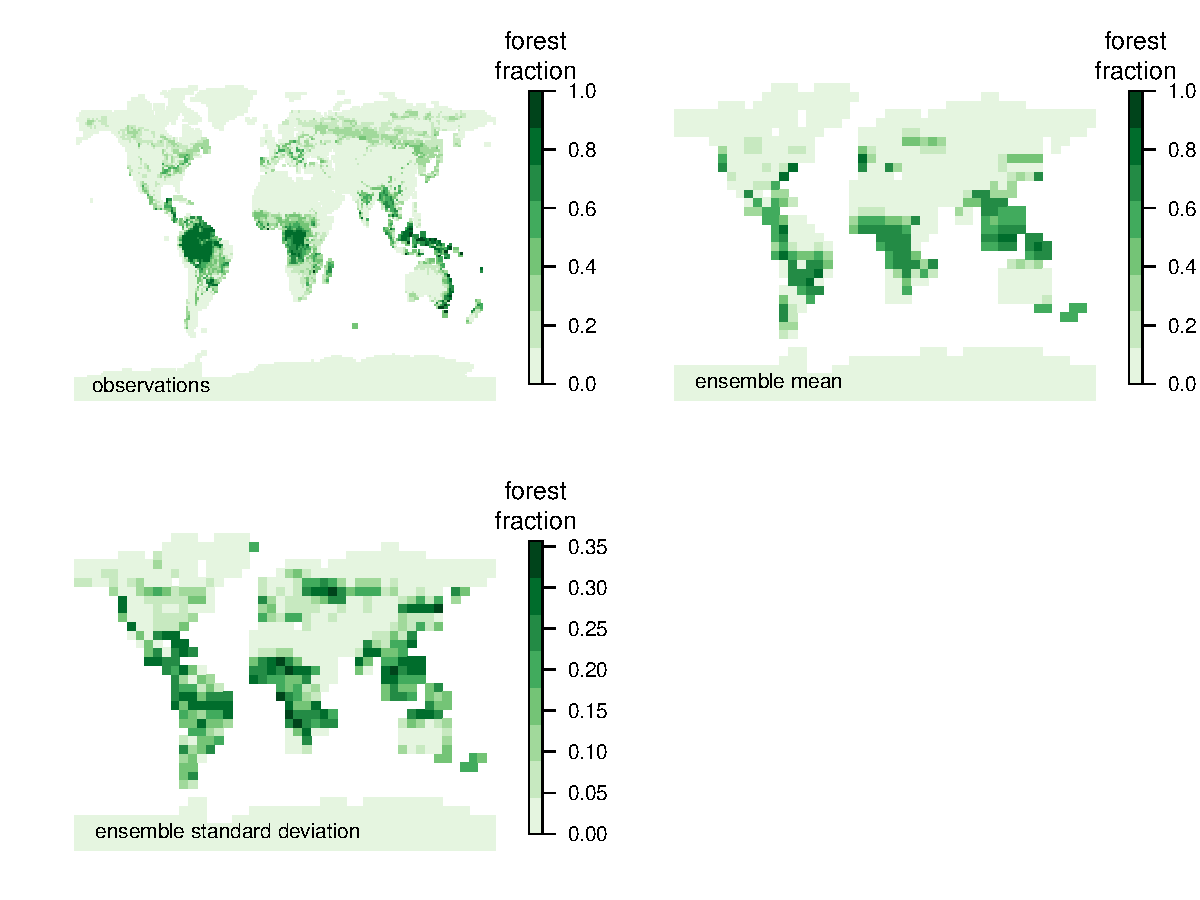
\includegraphics[width=12cm]{graphics/BL_obs_ensemble_mean_sd.pdf}
\caption{Observations of Broadleaf forest fraction (top left). Mean (top right) and standard deviation (bottom left) of broadleaf forest fraction across the 100 member ensemble of FAMOUS.}
\label{fig:BL_obs_ensemble_mean_sd}
\end{figure}

\begin{figure}[t]
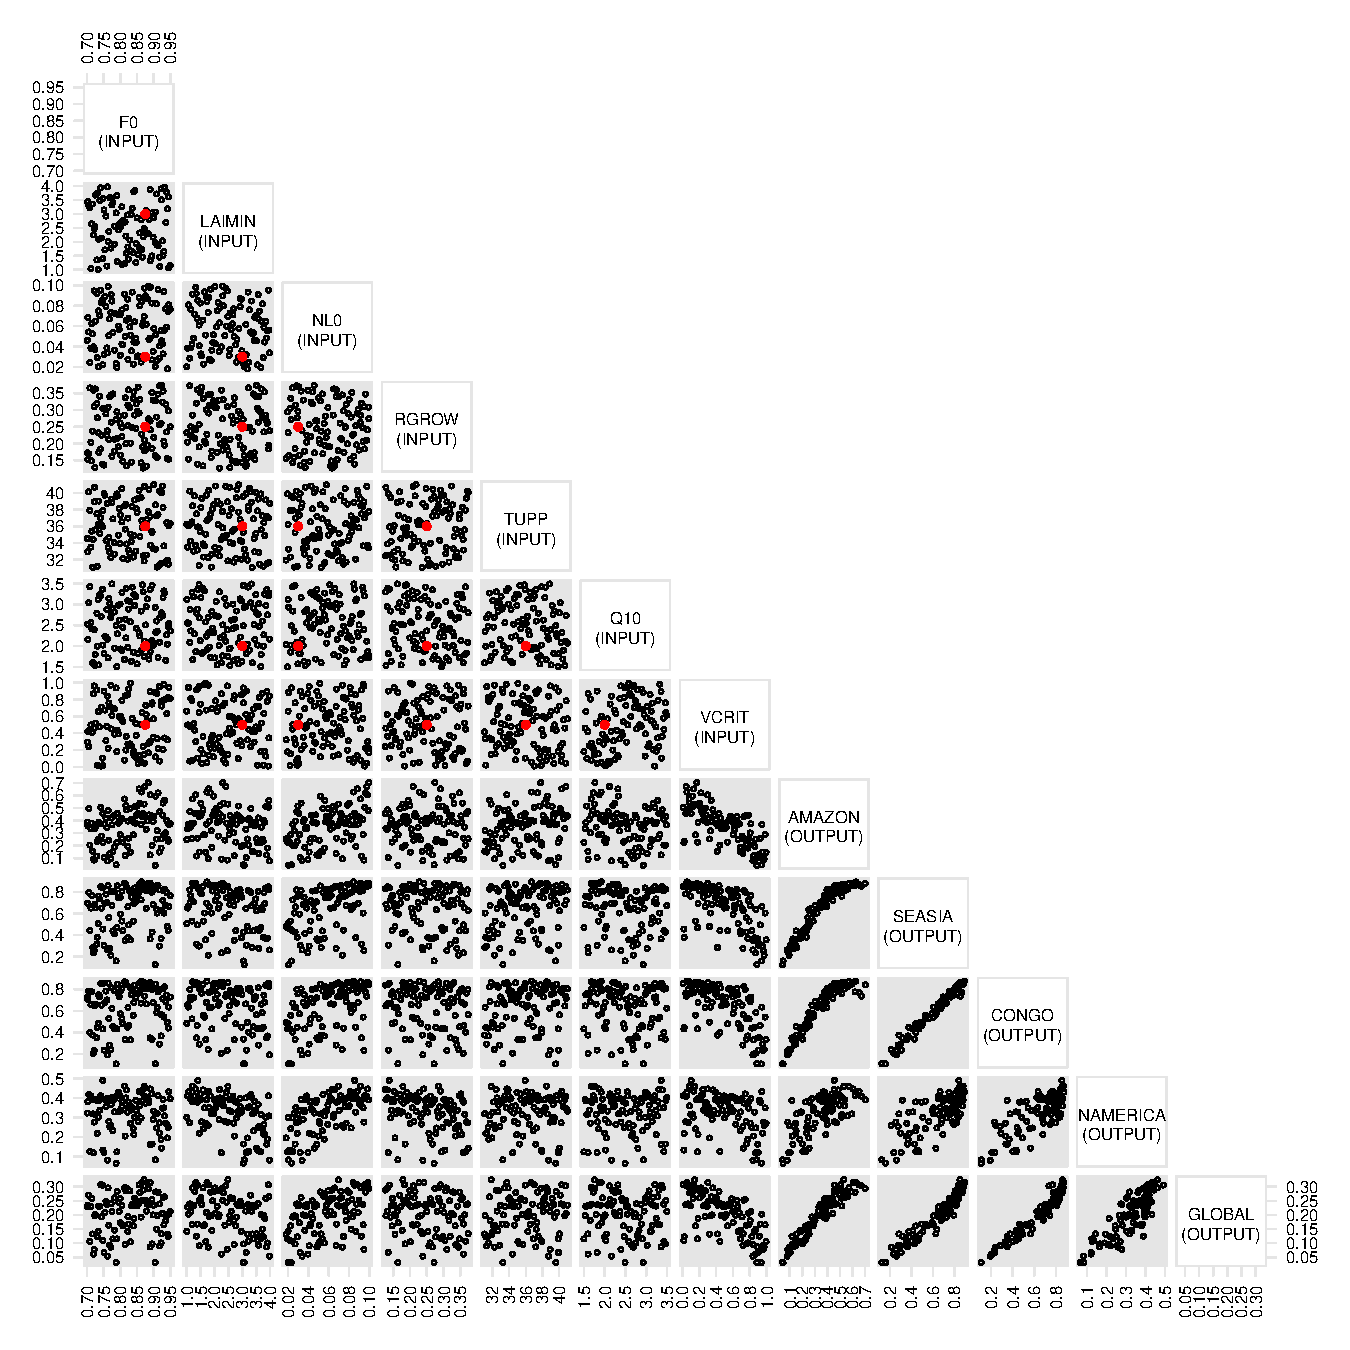
\includegraphics[width=12cm]{graphics/frac_pairs.pdf}
\caption{FAMOUS input parameters and forest fraction parameters, plotted against each other. \DIFaddbeginFL \DIFaddFL{Default inputs (not run) are marked in red.}\DIFaddendFL }
\label{fig:frac_pairs}
\end{figure}

\begin{figure}[t]
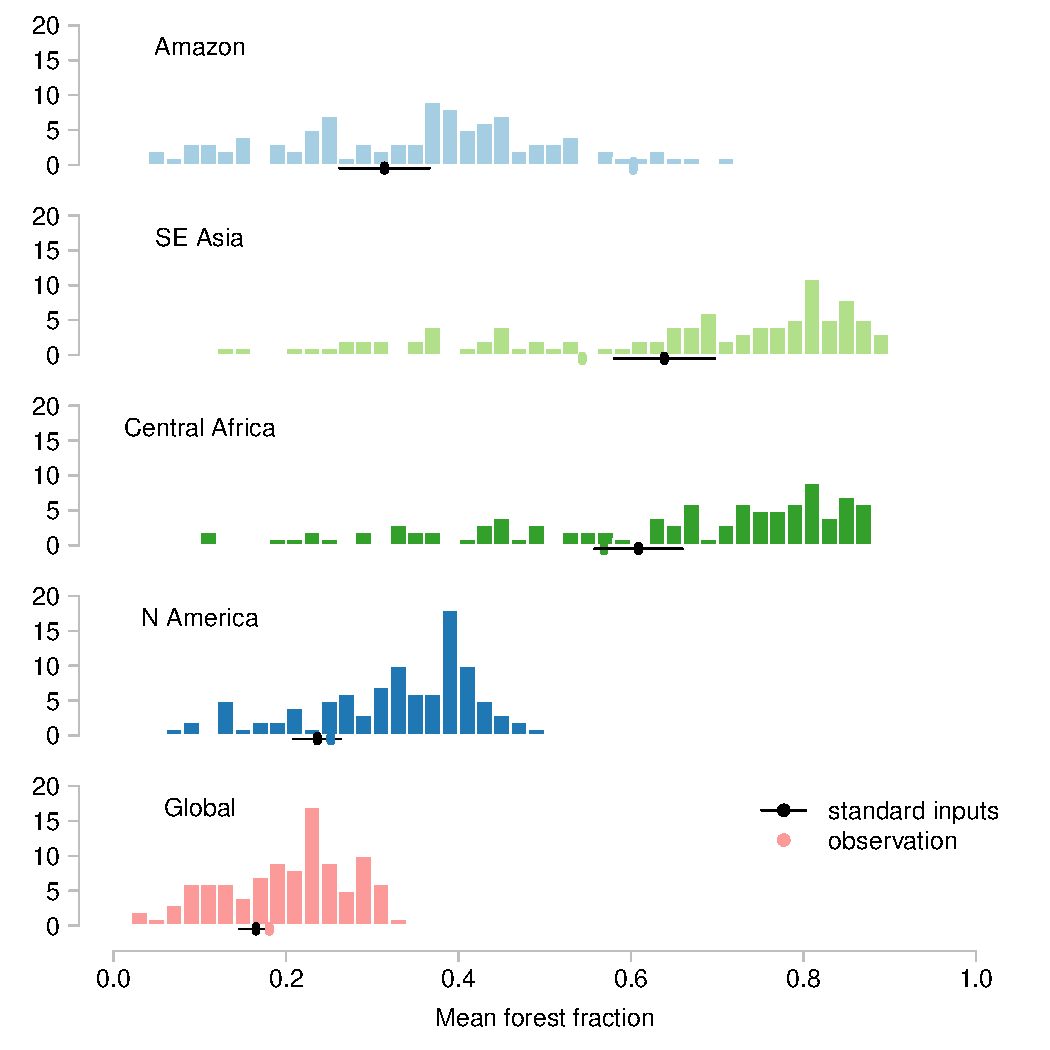
\includegraphics[width=12cm]{graphics/fraction_histogram_with_discrepancy_standard.pdf}
\caption{Histograms representing the number of ensemble members of a particular forest fraction in each region, and globally. Points plotted below the histograms represent the observed forest fraction (colours), \DIFdelbeginFL \DIFdelFL{and12cm }\DIFdelendFL \DIFaddbeginFL \DIFaddFL{and }\DIFaddendFL the forest fraction simulated at the "standard" parameters $\pm$1 standard deviation (black).}
\label{fig:fraction_histogram_with_discrepancy_standard}
\end{figure}

\begin{figure}[t]
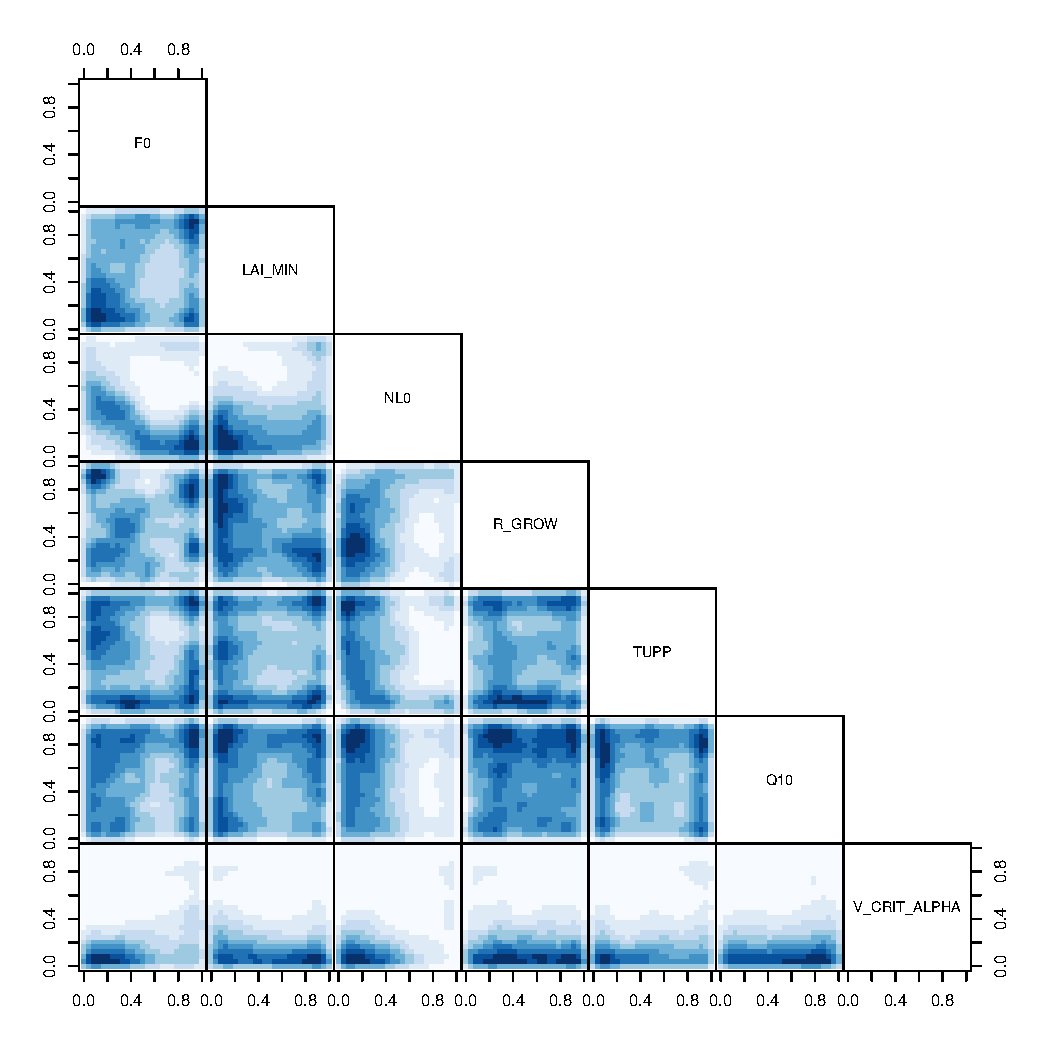
\includegraphics[width=12cm]{graphics/credible_NROY.pdf}
\caption{A density pairs plot of two dimensional projections of parameter space. The blue areas represent the density of NROY points, using all of the data, with an assumed observational uncertainty of 0.05 (1 standard deviation).}
\label{fig:credible_NROY}
\end{figure}

\begin{figure}[t]
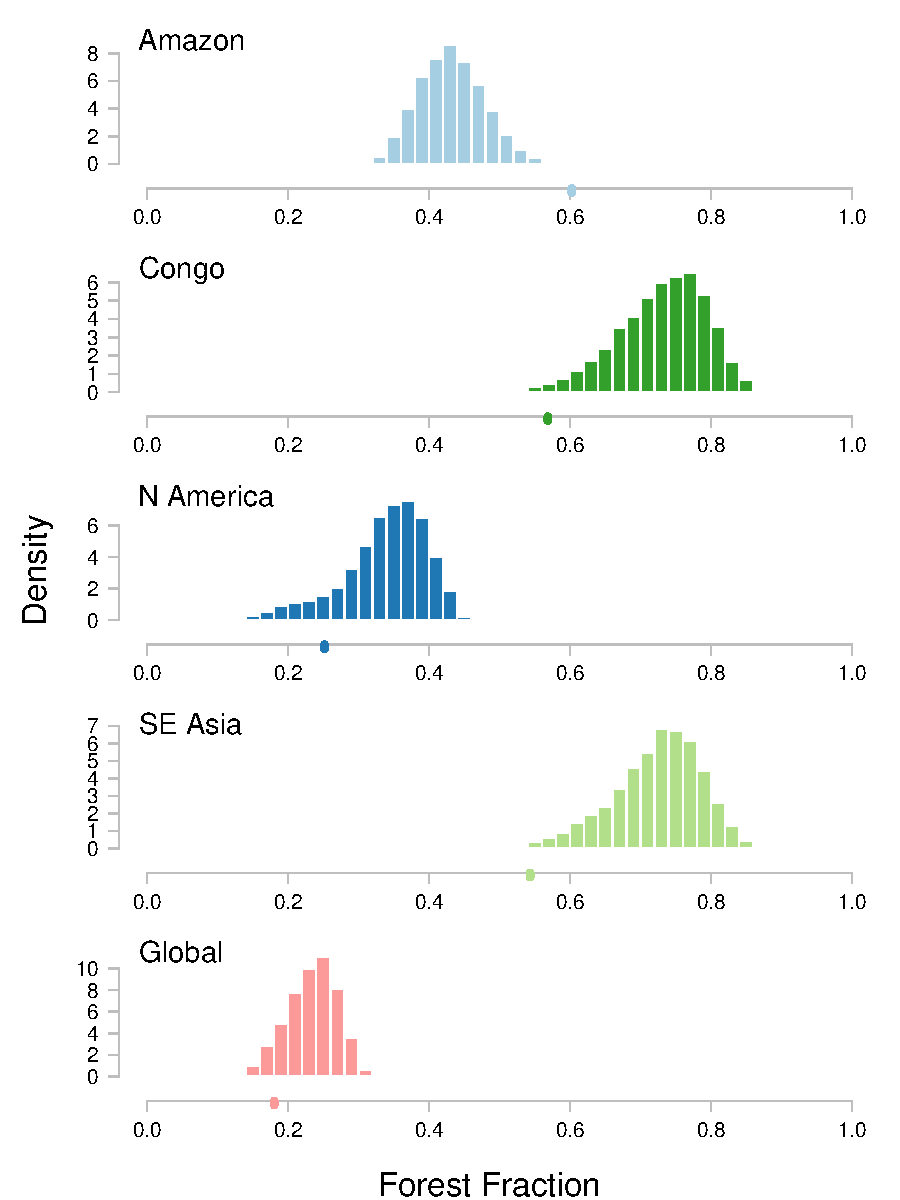
\includegraphics[width=12cm]{graphics/credible_NROY_hists.pdf}
\caption{Best-estimate draws of forest fraction output from the emulator, at the set of points Not Ruled Out Yet when assuming a credible observational uncertainty. The value of the observed forest fractions are are plotted as a single point on the corresponding x-axes (a ``rug plot'').}
\label{fig:credible_NROY_hists}
\end{figure}

\begin{figure}[t]
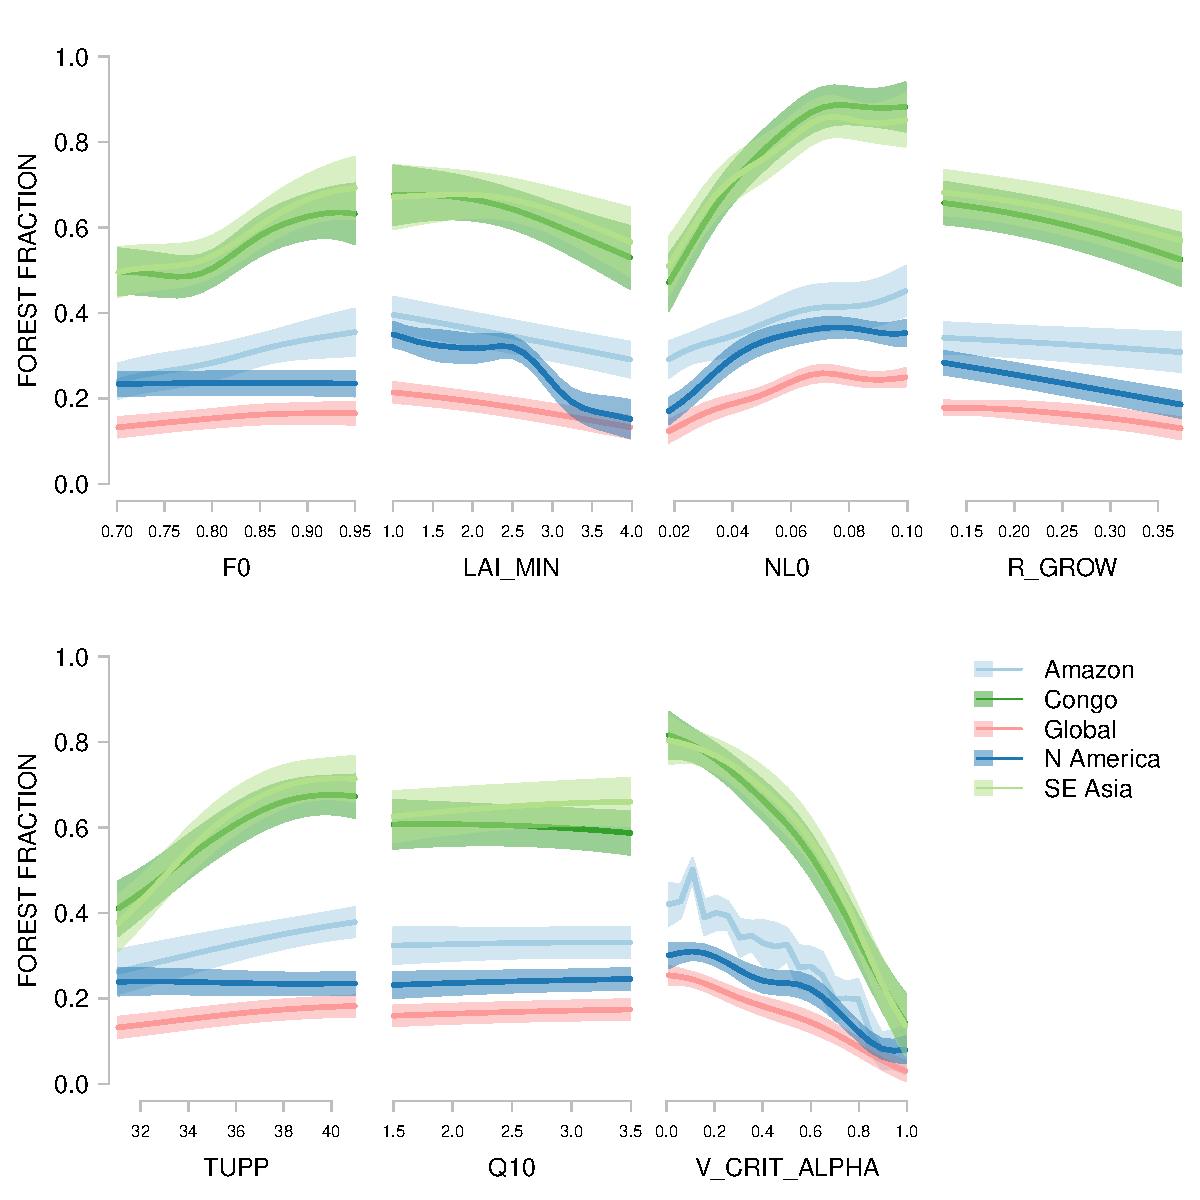
\includegraphics[width=12cm]{graphics/amaz_oat_sens.pdf}
\caption{Marginal sensitivity of mean forest fraction to each input parameter in turn, with all other parameters held at standard values. Central lines represent the emulator mean, and shaded areas represent the estimate of emulator uncertainty, at the $\pm$1 standard deviation level.}
\label{fig:amaz_oat_sens}
\end{figure}

\begin{figure}[t]
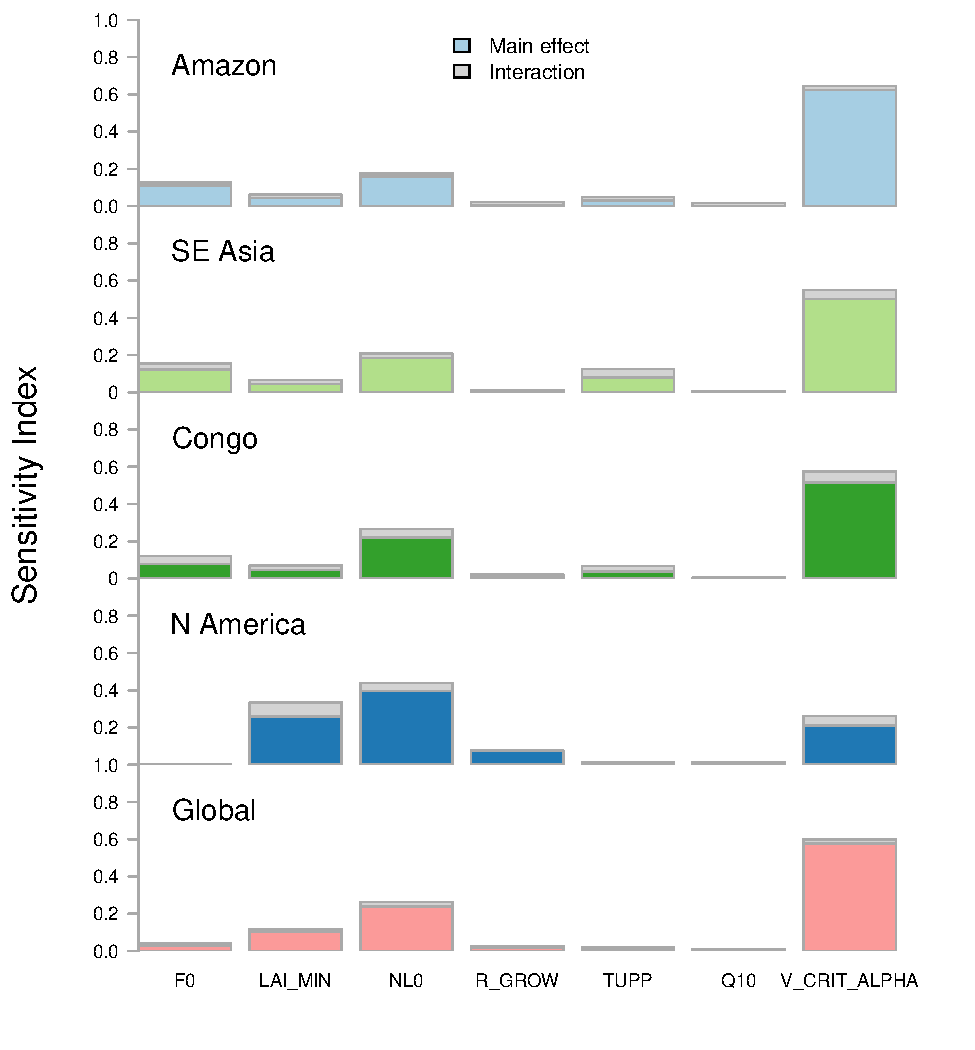
\includegraphics[width=12cm]{graphics/FAST_histograms.pdf}
\caption{Sensitivity analysis of forest fraction via the FAST algorithm of \cite{saltelli1999sensitivity}.}
\label{fig:FAST_histograms}
\end{figure}

\begin{figure}[t]
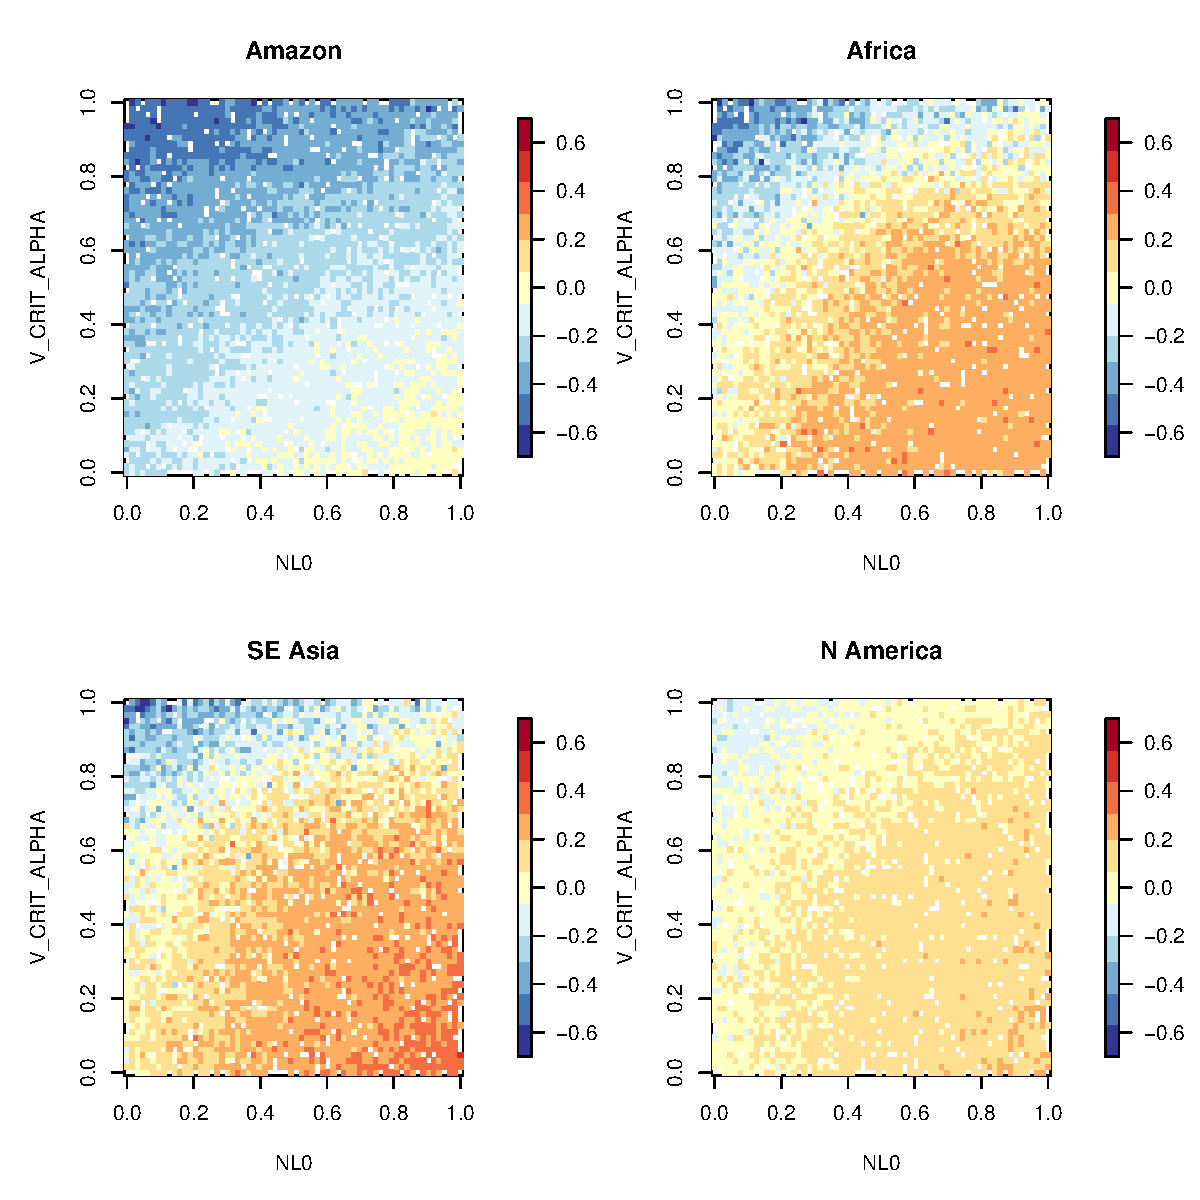
\includegraphics[width=12cm]{graphics/discrepancy_parameter_space.pdf}
\caption{Maps of simulator error, in units of forest fraction, when projected into the two dimensional space of the most active parameters, NL0 and V\_CRIT\_ALPHA.}
\label{fig:discrepancy_parameter_space}
\end{figure}

\begin{figure}[t]
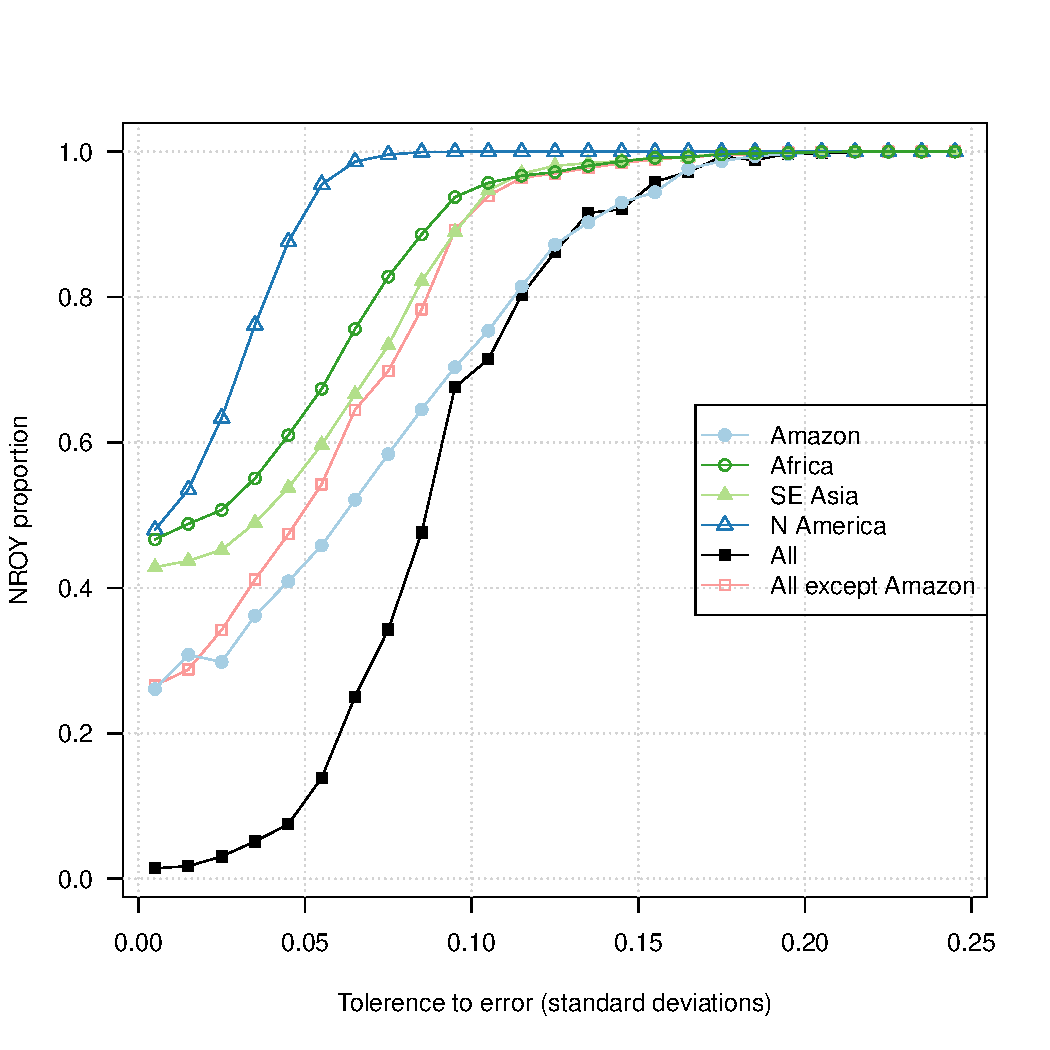
\includegraphics[width=12cm]{graphics/Prop_NROY_tolerance_unc.pdf}
\caption{Proportion of NROY (Not Ruled Out Yet) input space plotted against ``tolerence to error'' - the total error budget including emulator, observational and simulator discrepancy uncertainty.}
\label{fig:Prop_NROY_tolerance_unc}
\end{figure}

%\begin{figure}[t]
%DIF < 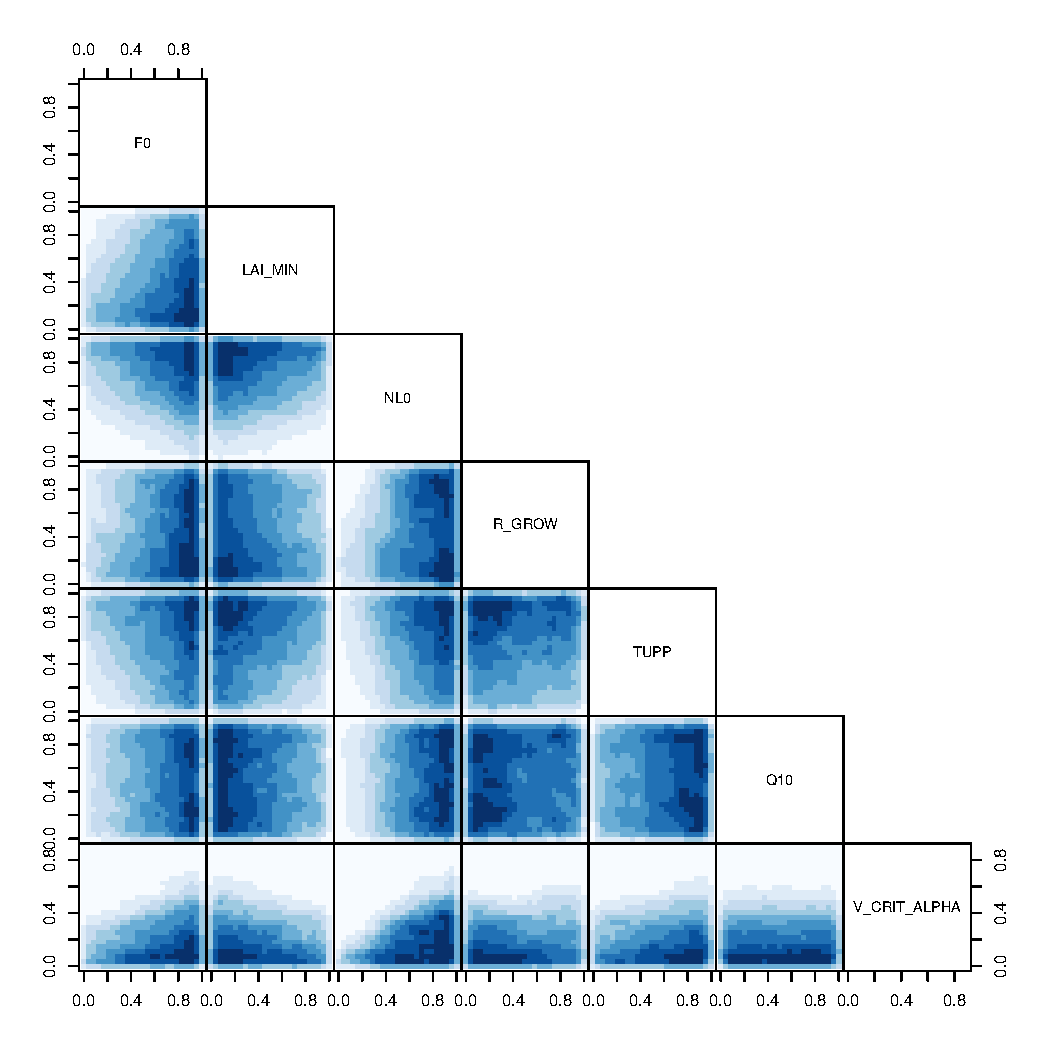
\includegraphics[width=12cm]{graphics/best_inputs_amazon.pdf}
%DIF > 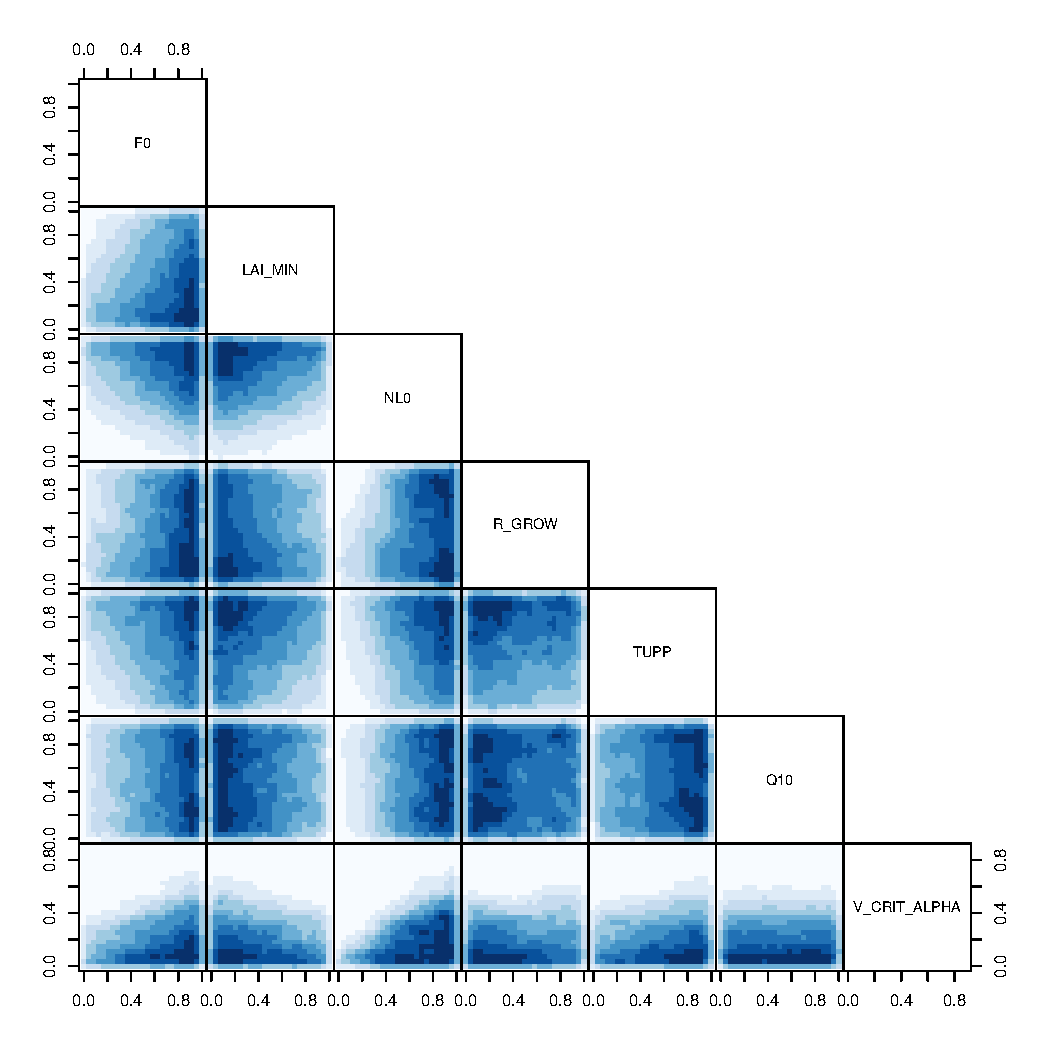
\includegraphics[width=8.3cm]{graphics/best_inputs_amazon.pdf}
%\caption{TEXT}
%\label{fig:best_inputs_amazon}
%\end{figure}

\begin{figure}[t]
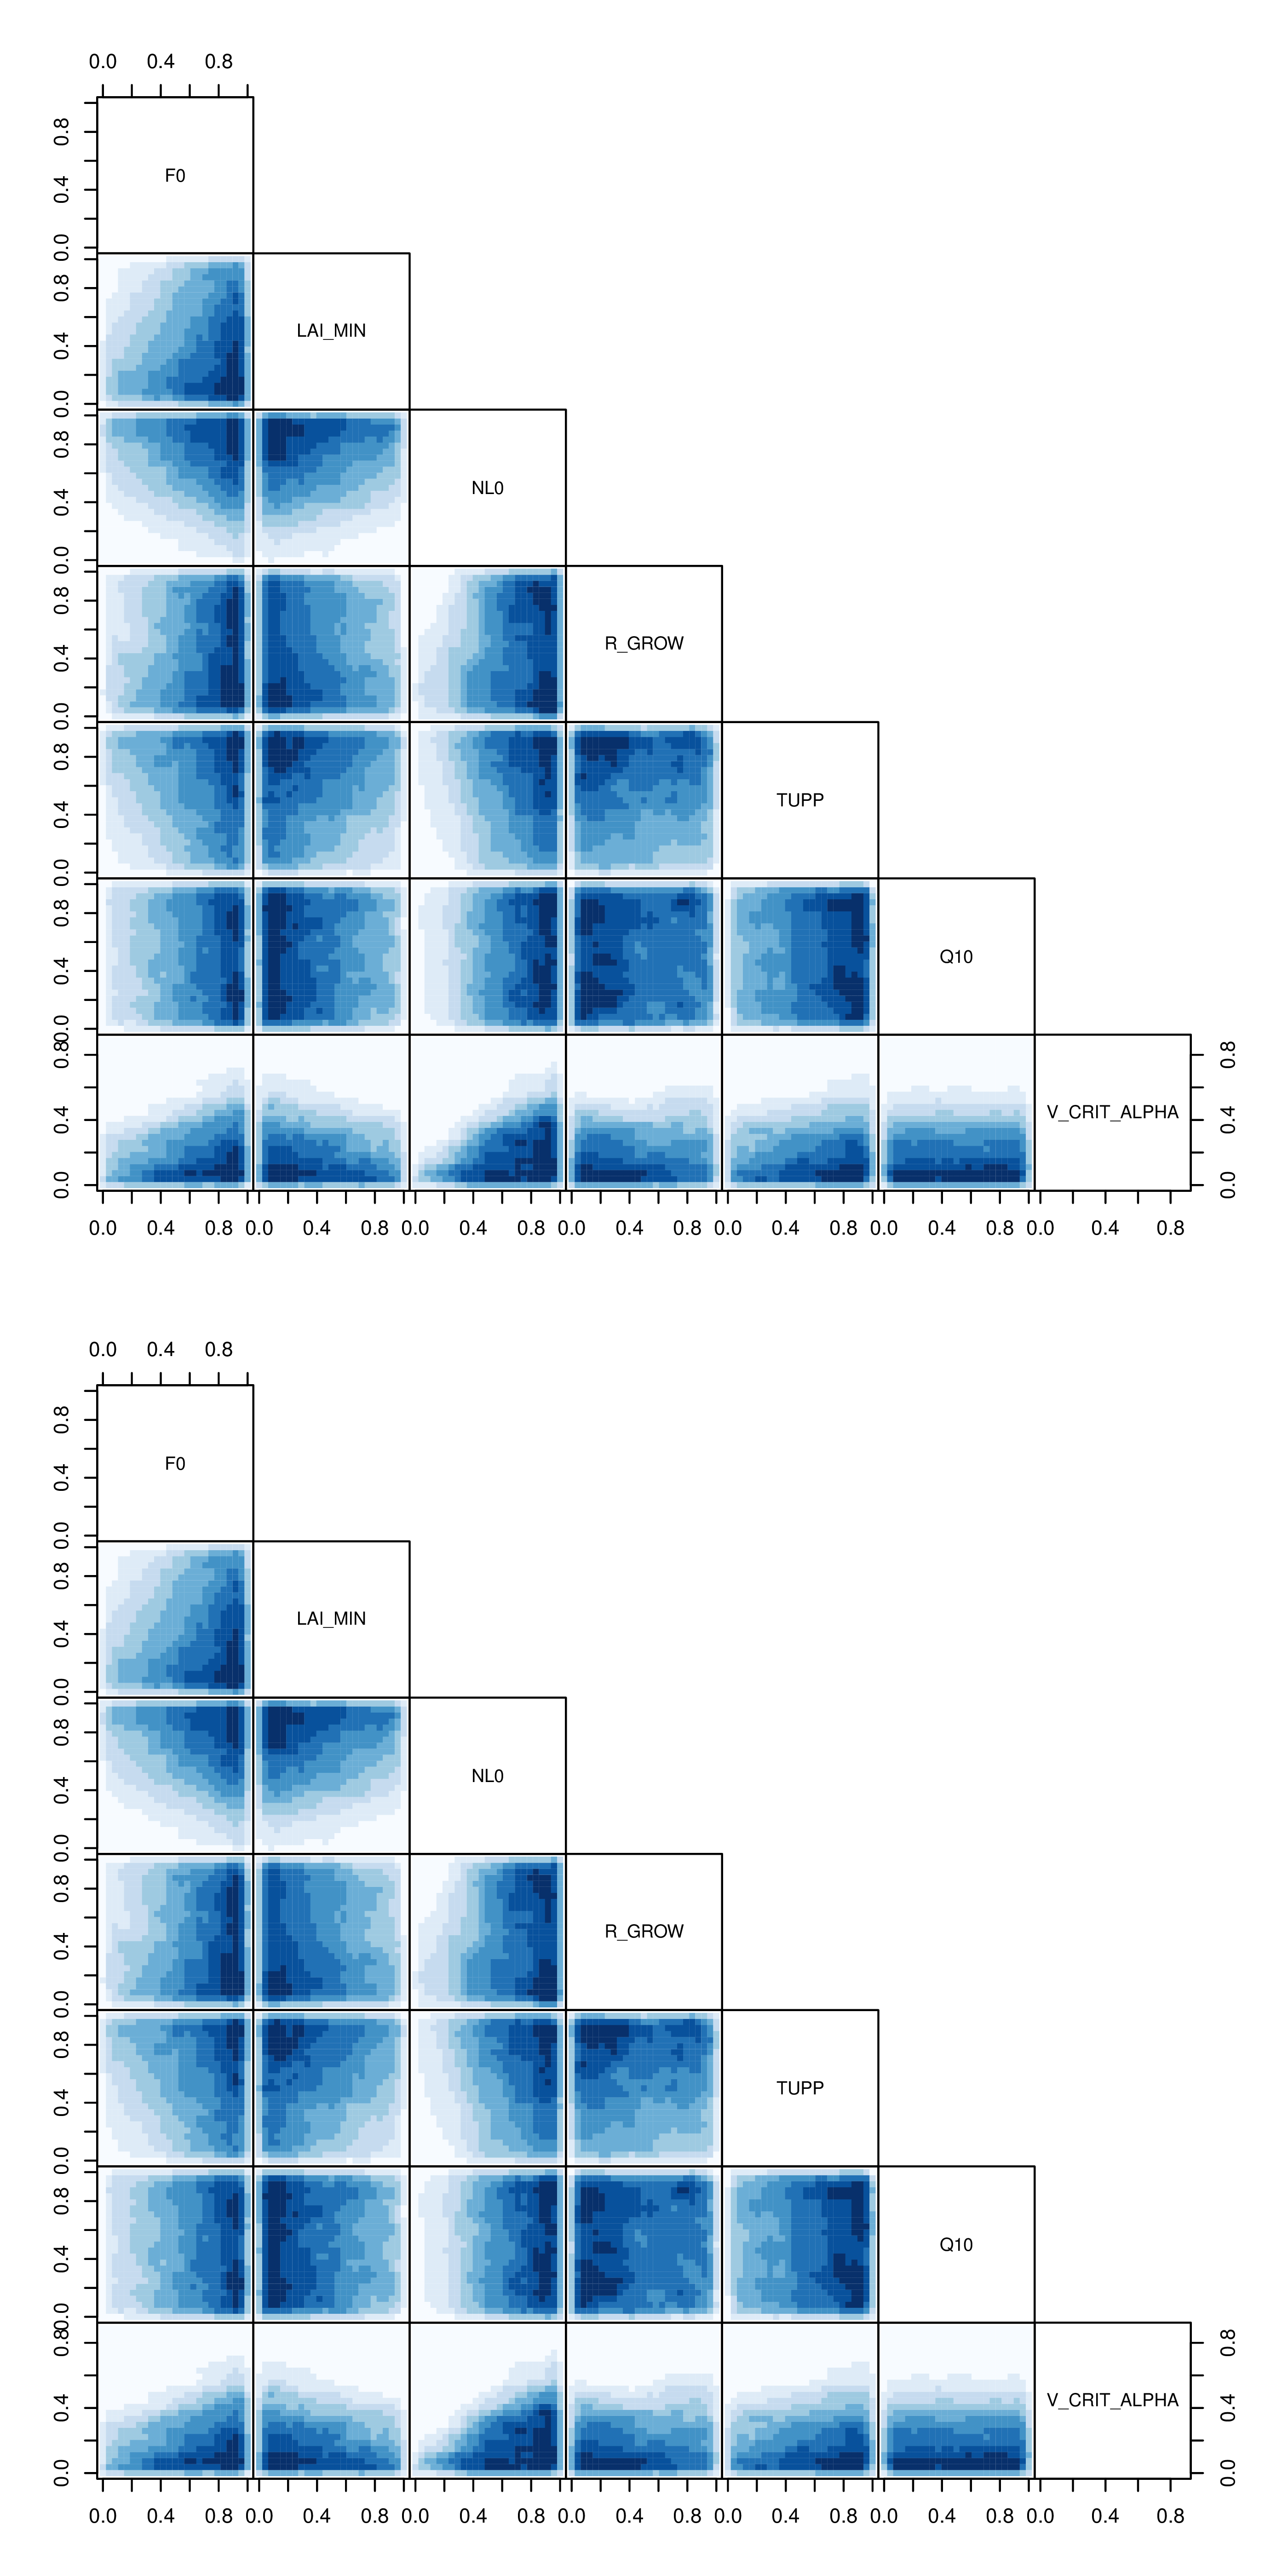
\includegraphics[width=8.3cm]{graphics/best_inputs.png}
\caption{Marginal density of input parameter sets consistent with a very low ``tolerance to error'', and perfect observations, for the North American, Southeast Asian and Central African forests combined (top) and the Amazon (bottom). Dark blue regions indicate those with the highest concentration of NROY candidates, and therefore most compatible with the observations.}
\label{fig:best_inputs}
\end{figure}

%\begin{figure}[t]
%DIF < 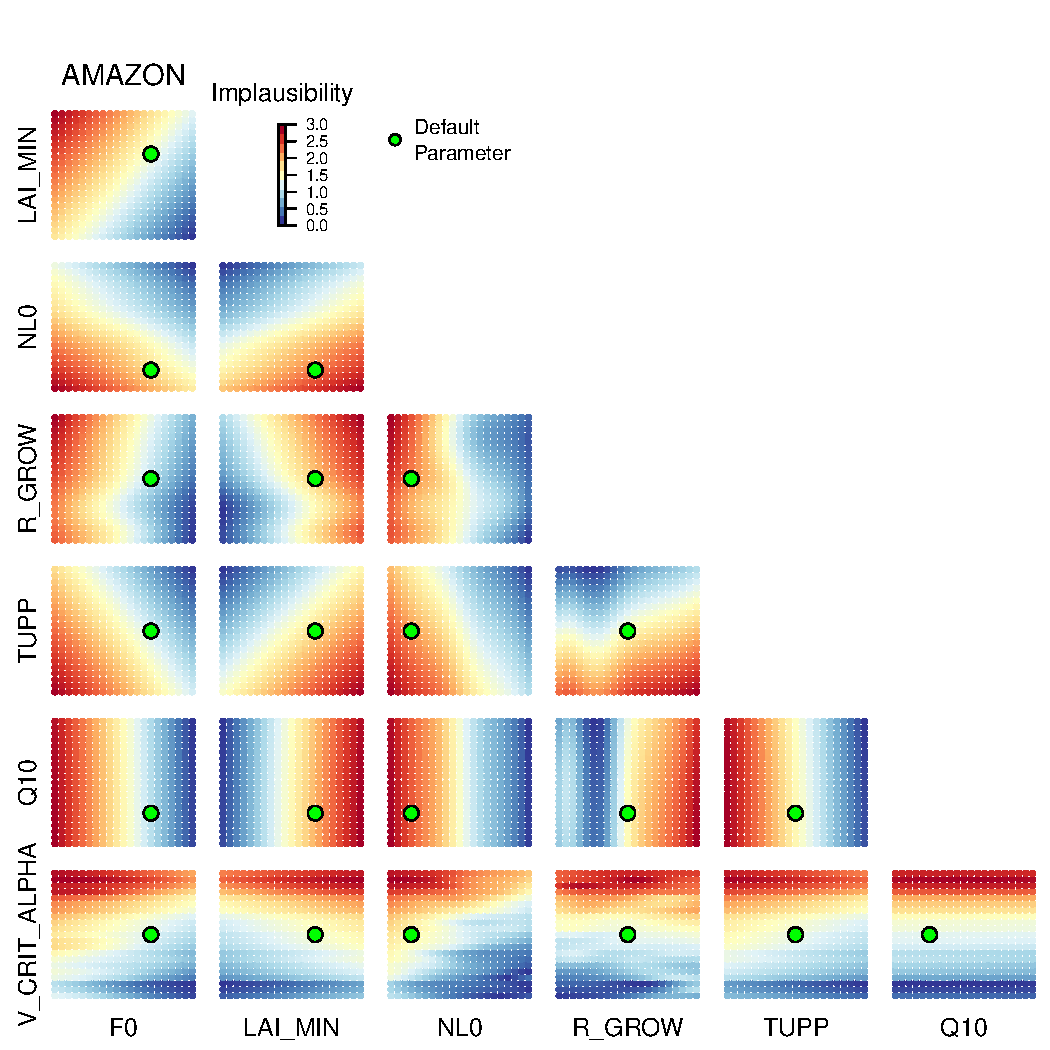
\includegraphics[width=12cm]{graphics/taat_amaz.pdf}
%DIF > 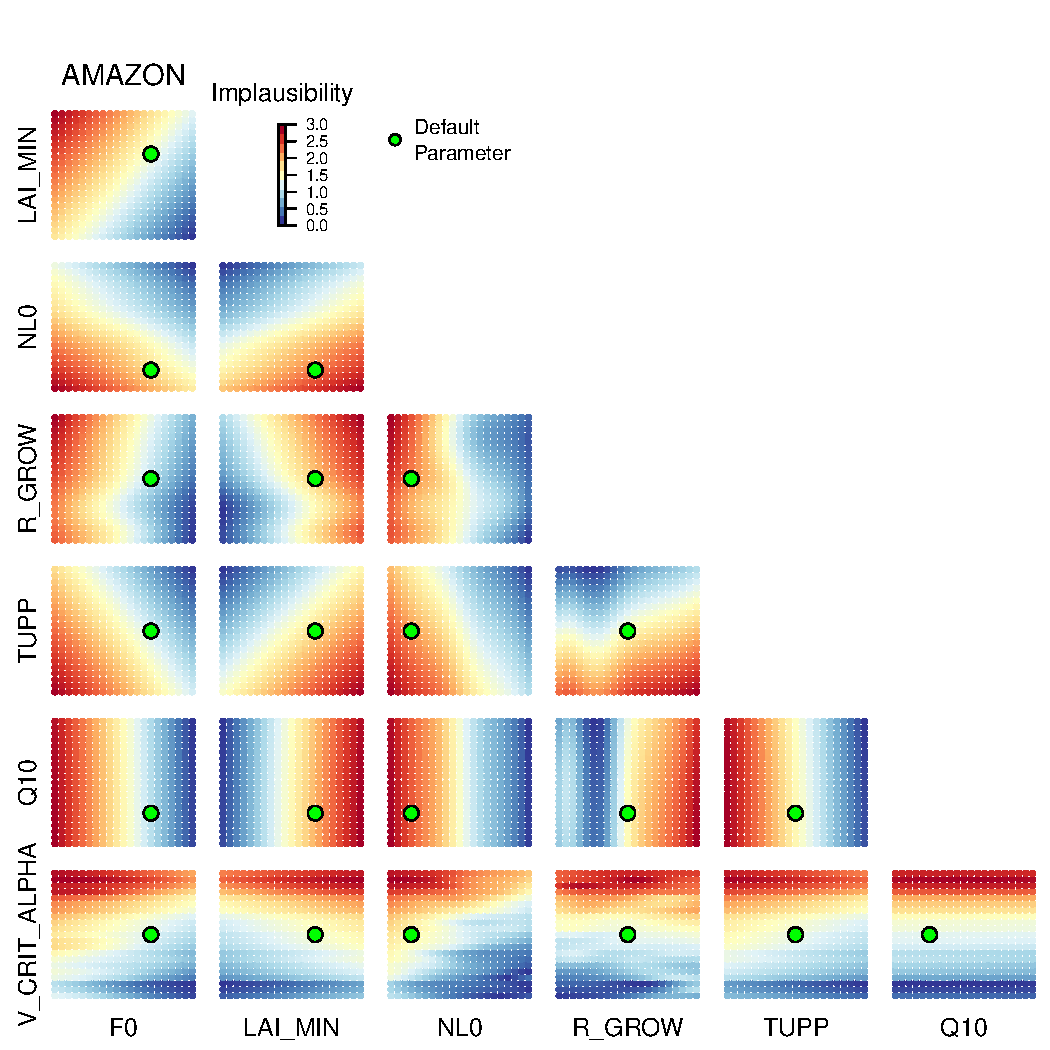
\includegraphics[width=8.3cm]{graphics/taat_amaz.pdf}
%\caption{TEXT}
%\label{fig:taat_amaz}
%\end{figure}



\begin{figure}[t]
\DIFdelbeginFL %DIFDELCMD < 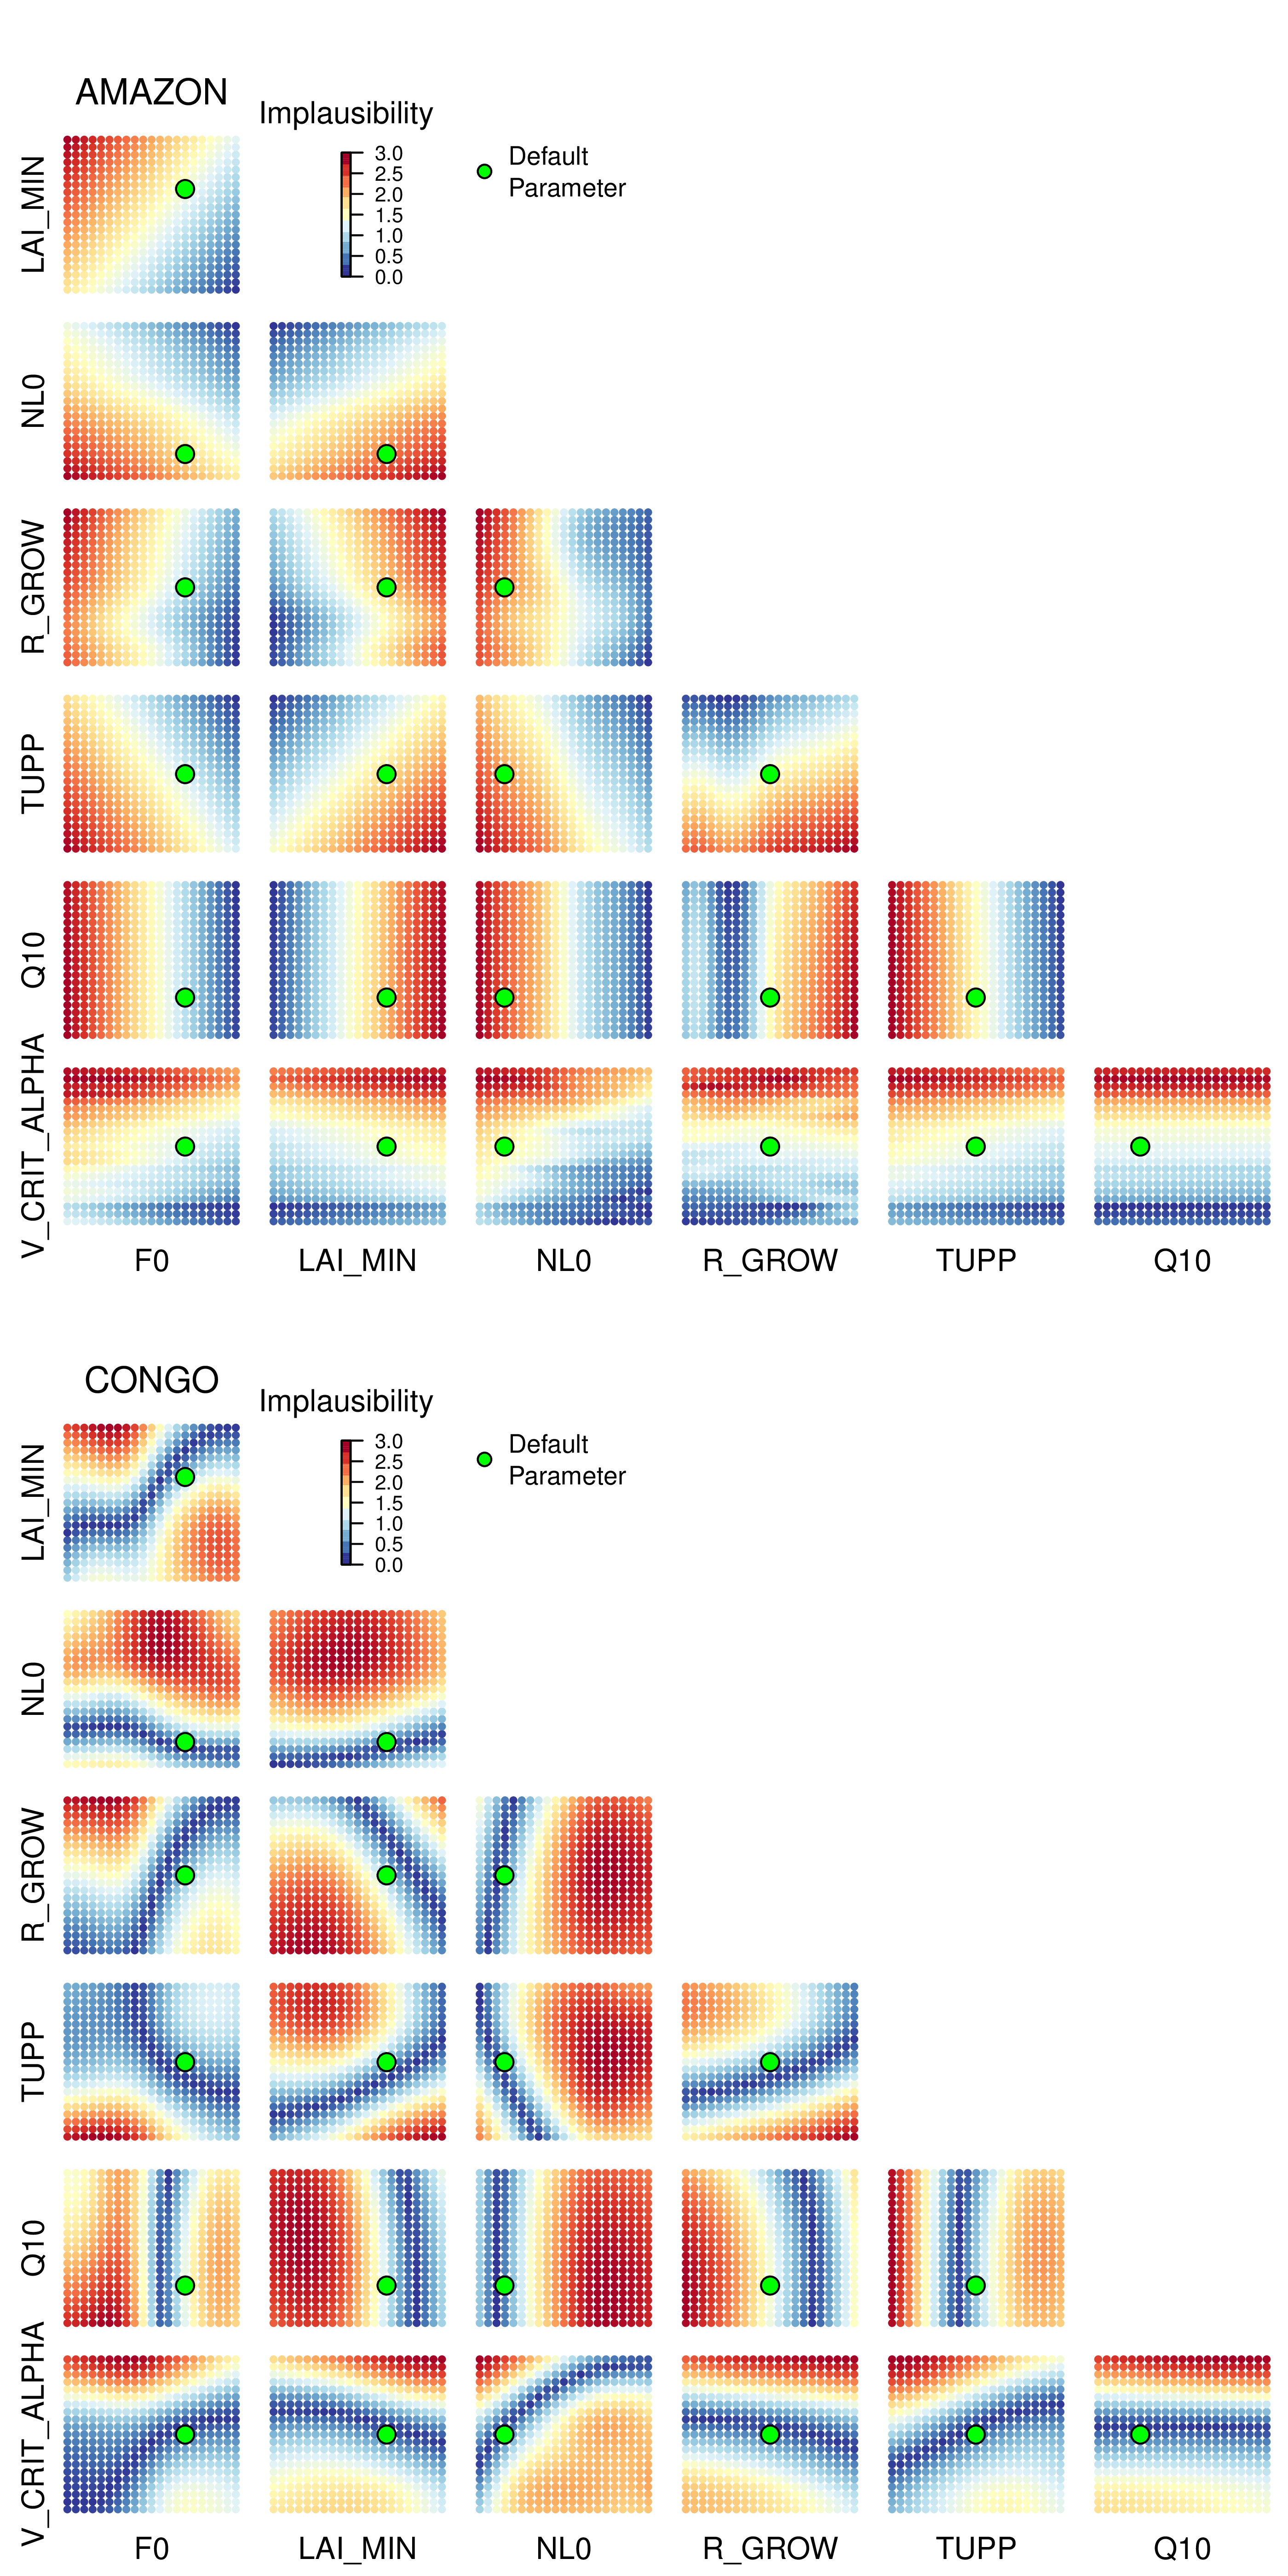
\includegraphics[width=8.3cm]{graphics/taat.png}
%DIFDELCMD < %%%
%DIFDELCMD < \caption{%
{%DIFAUXCMD
\DIFdelFL{Implausibility, given a ``tolerance to error'' of 0.1, varying two parameters at a time and holding all others at their default values. Amazon forest (top) and Central African forest (bottom). Blue indicates regions where the model best simulates the individual option, while red indicates regions where the model simulates the forests more poorly. The green point indicates the location of the ``standard'' set of parameters for FAMOUS in the varied dimensions.}}
%DIFAUXCMD
%DIFDELCMD < \label{fig:taat}
%DIFDELCMD < \end{figure}
%DIFDELCMD < 

%DIFDELCMD < \begin{figure}[t]
%DIFDELCMD < %%%
\DIFdelendFL 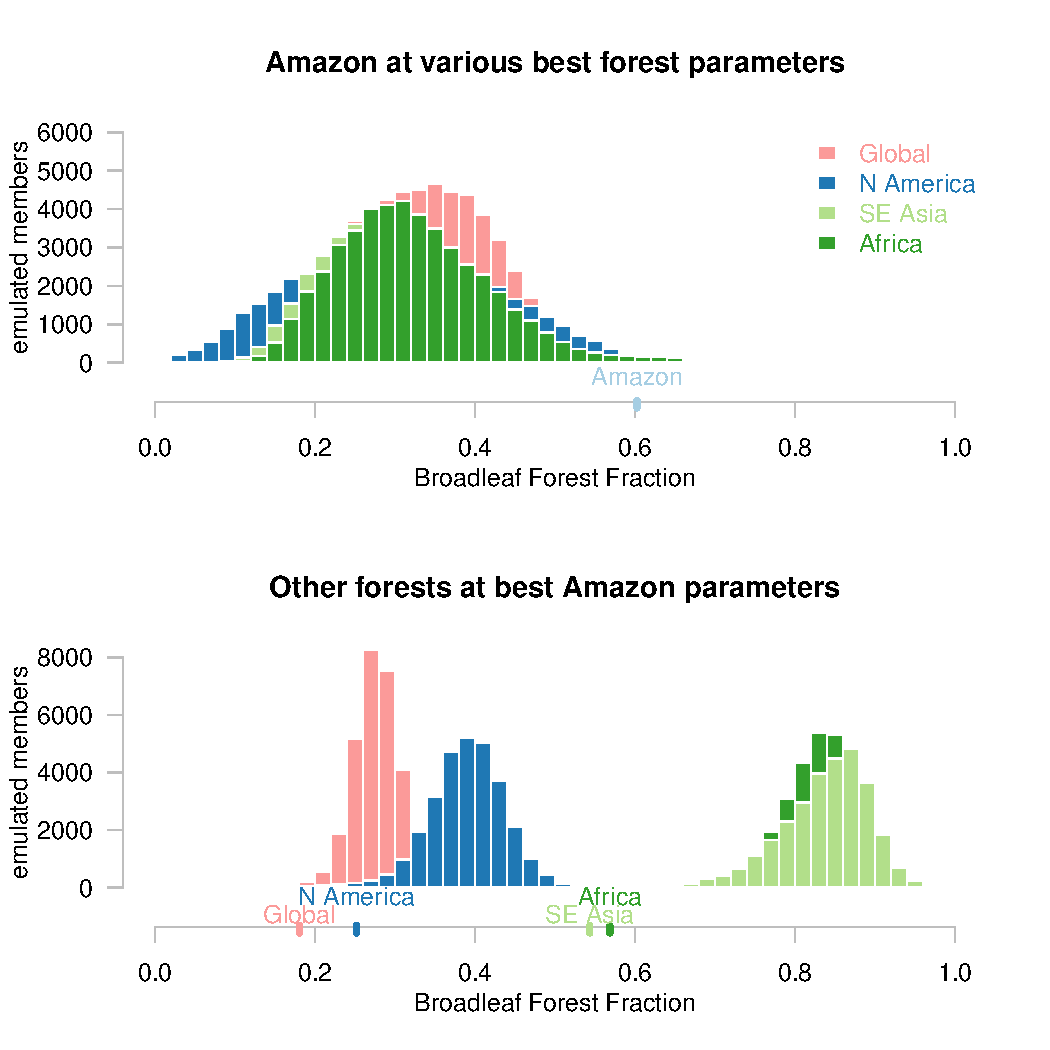
\includegraphics[width=12cm]{graphics/best_inputs_swaps_hists_Paired.pdf}
\caption{(Top) Forest fraction in the FAMOUS Amazon at the set of parameters where the FAMOUS best matches each of the other forest observations. (Bottom) Other forests in FAMOUS at the set where the FAMOUS Amazon best matches observations. Observed forest fractions are shown as marks underneath the histograms.}
\label{fig:best_inputs_swaps_hists_Paired}
\end{figure}

\begin{figure}[t]
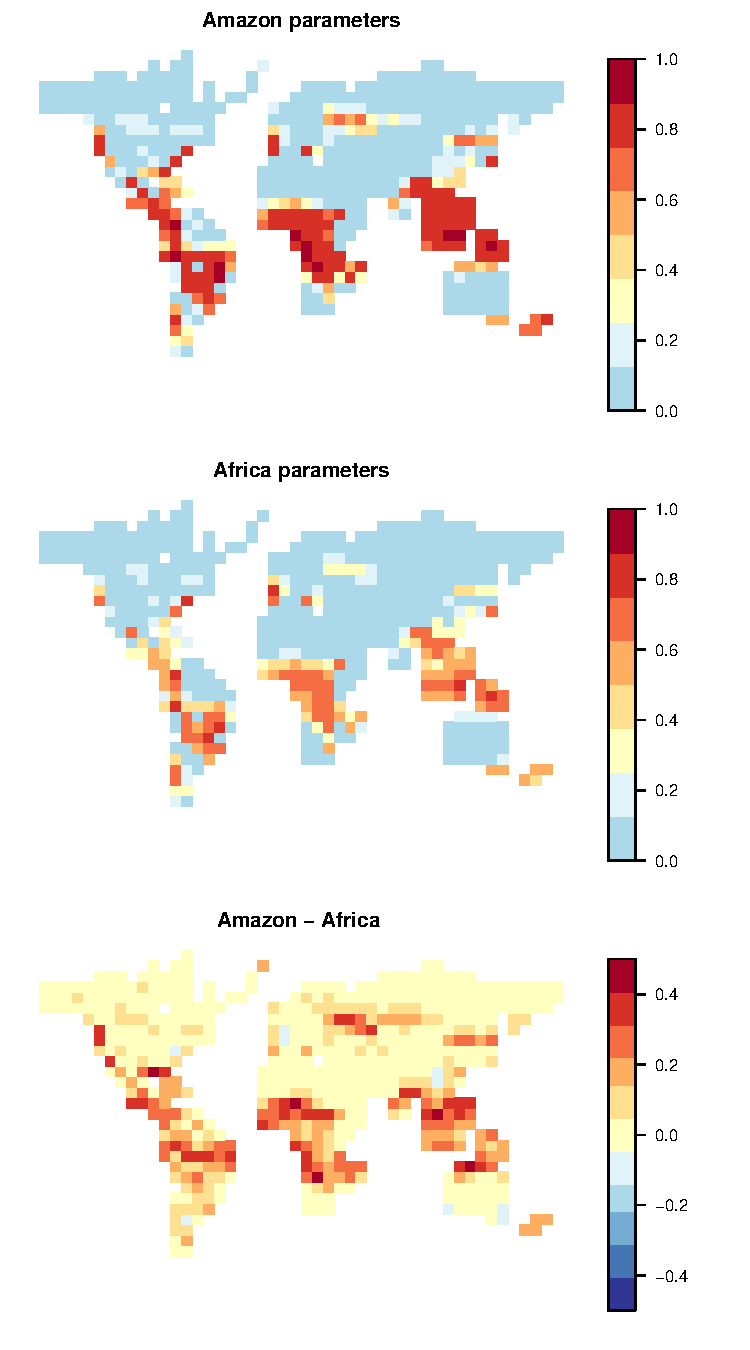
\includegraphics[width=8.3cm]{graphics/best_X_maps.pdf}
\caption{Maps of mean broadleaf forest fraction, over the ``best'' set of parameters found for the Amazon (top) and the Central African forest (centre). The difference between the two is mapped at the bottom.}
\label{fig:best_X_maps}
\end{figure}

\begin{figure}[t]
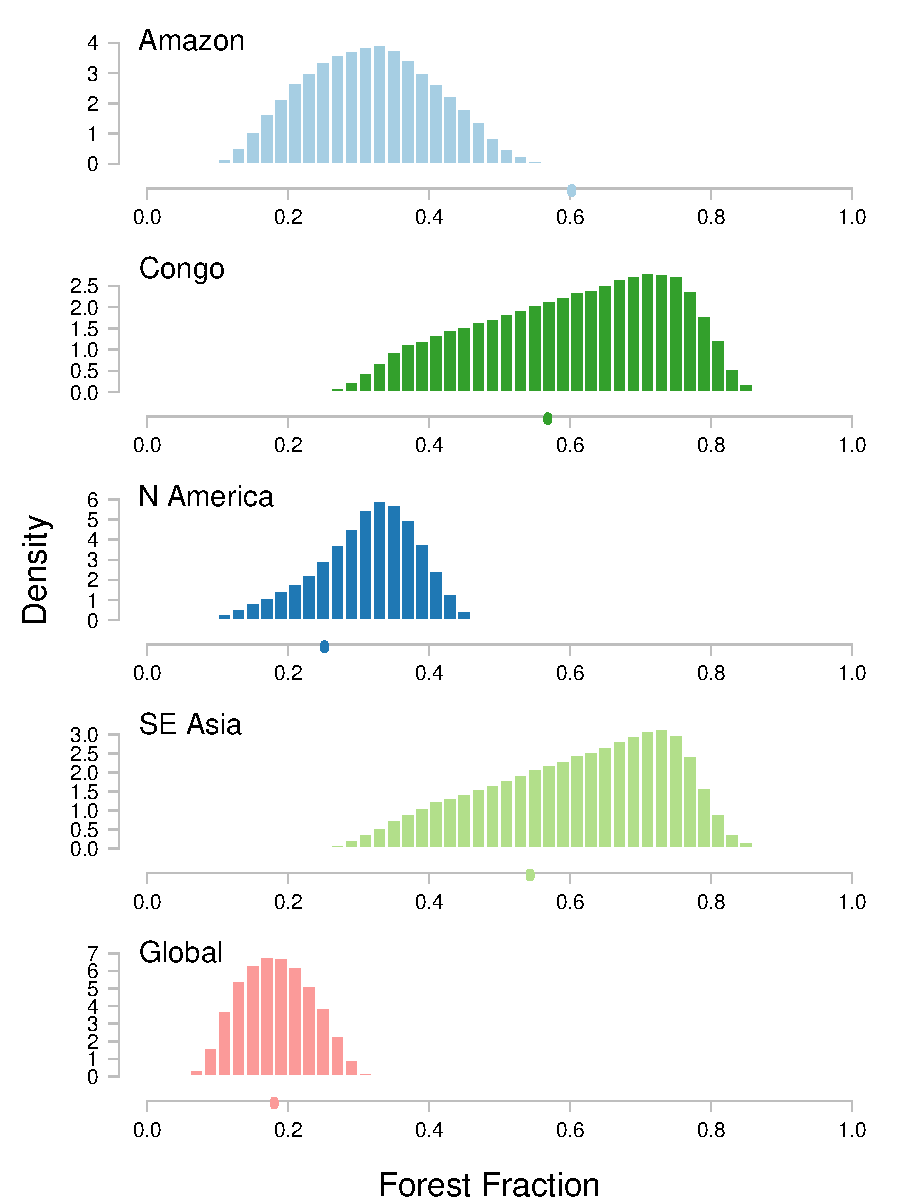
\includegraphics[width=12cm]{graphics/credible_NROY_hists_disc.pdf}
\caption{Histograms of emulated simulator output using credible estimates for observational uncertainty, a \DIFdelbeginFL \DIFdelFL{model }\DIFdelendFL \DIFaddbeginFL \DIFaddFL{simulator }\DIFaddendFL discrepancy term for the Amazon, and credible discrepancy uncertainty.}
\label{fig:credible_NROY_hists_disc}
\end{figure}

\begin{figure}[t]
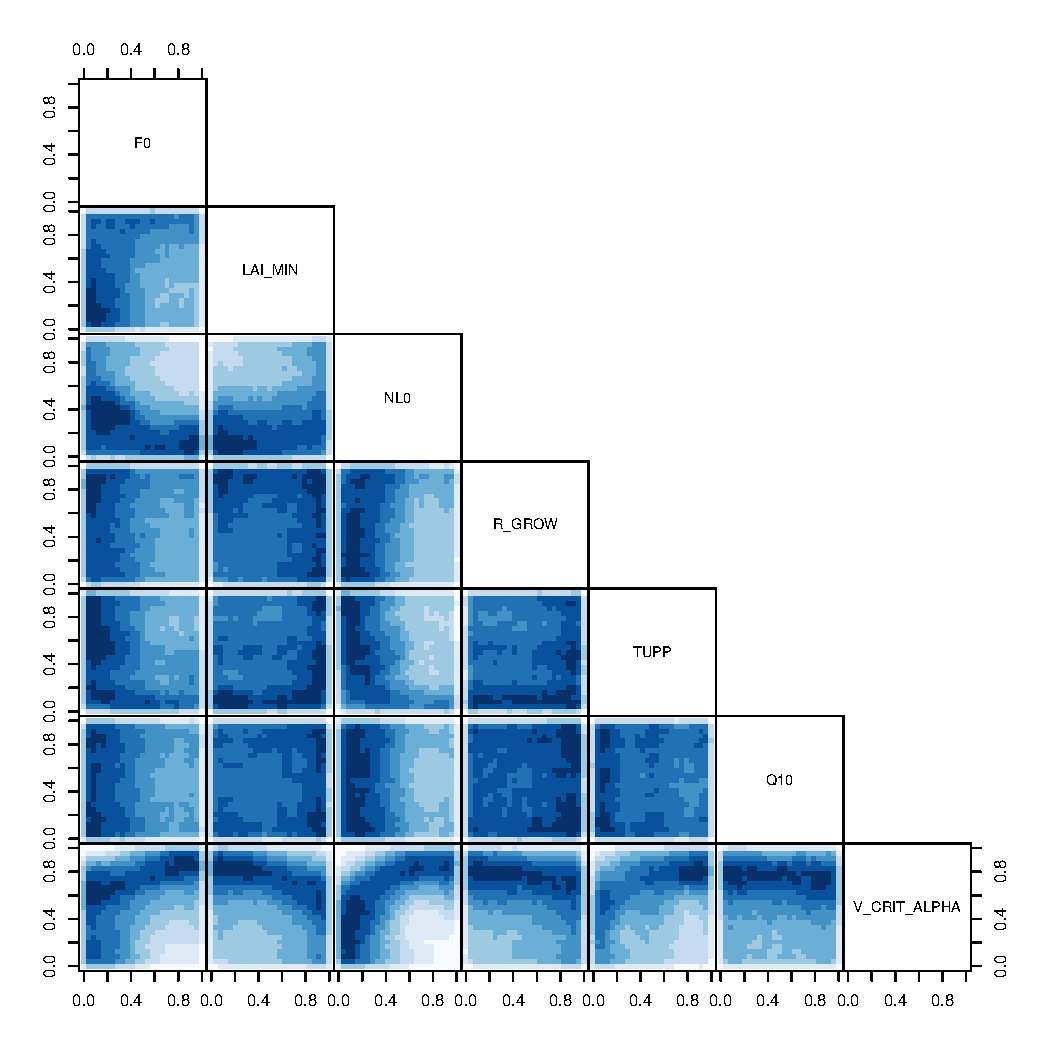
\includegraphics[width=12cm]{graphics/plausible_disc_input_space.pdf}
\caption{A density plot of the two dimensional projections of NROY samples from the design input space, using a all forest observations and a discrepancy function for the Amazon.}
\label{fig:plausible_disc_input_space}
\end{figure}


\DIFdelbegin %DIFDELCMD < \begin{figure}[t]
%DIFDELCMD < 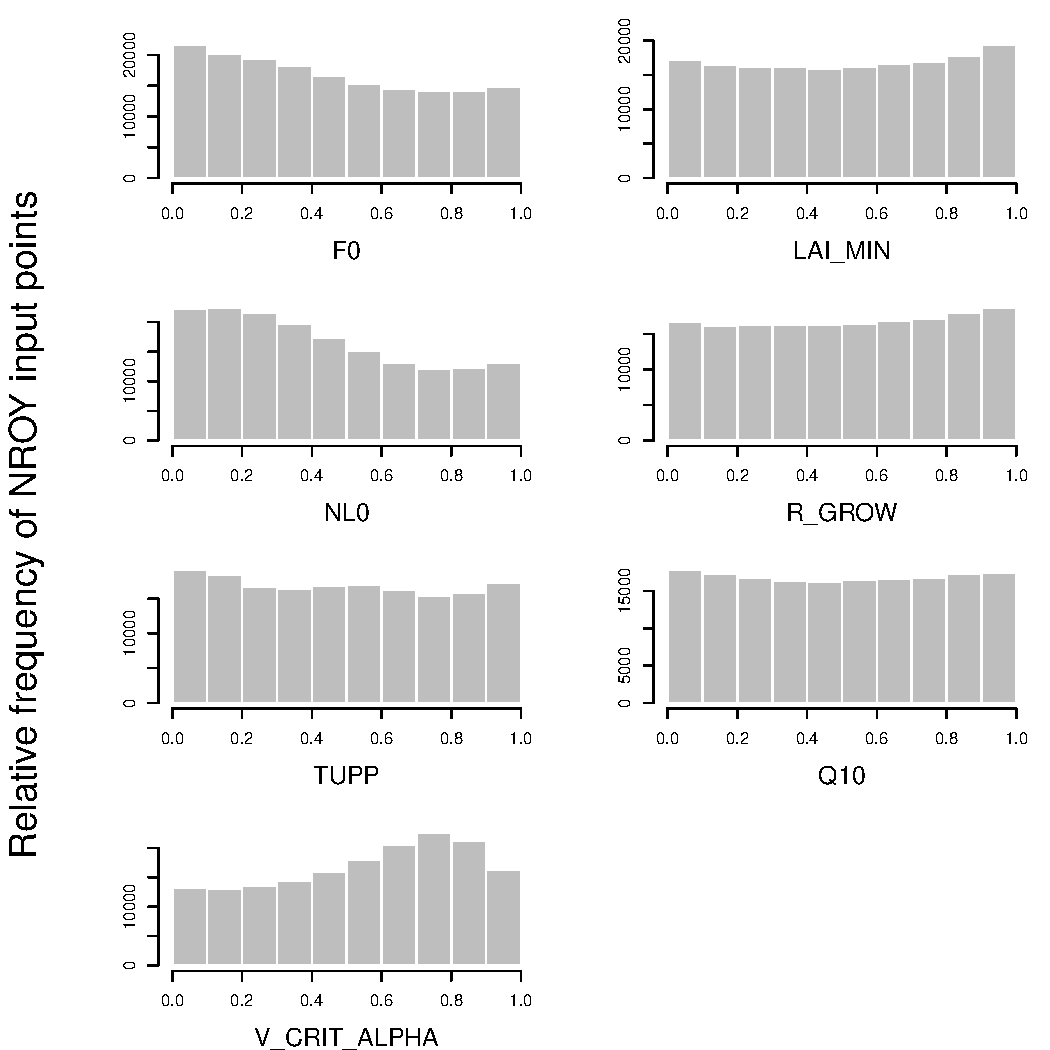
\includegraphics[width=12cm]{graphics/input_frequency_marginal.pdf}
%DIFDELCMD < %%%
%DIFDELCMD < \caption{%
{%DIFAUXCMD
\DIFdel{Marginal histograms of the relative frequency of NROY emulated input points in each dimension of parameter space, using all forest observations and a discrepancy function for the Amazon.}}
%DIFAUXCMD
%DIFDELCMD < \label{fig:input_frequency_marginal}
%DIFDELCMD < \end{figure}
%DIFDELCMD < 

%DIFDELCMD < %%%
\DIFdelend %\begin{figure}[t]
%DIF < \includegraphics[width=12cm]{graphics/.pdf}
%DIF > \includegraphics[width=8.3cm]{graphics/.pdf}
%\caption{TEXT}
%\label{fig:}
%\end{figure}



%% ONE-COLUMN FIGURES

%%f
%\begin{figure}[t]
%DIF < \includegraphics[width=12cm]{FILE NAME}
%DIF > \includegraphics[width=8.3cm]{FILE NAME}
%\caption{TEXT}
%\end{figure}
%
%%% TWO-COLUMN FIGURES
%
%%f
%\begin{figure*}[t]
%DIF < \includegraphics[width=12cm]{FILE NAME}
%DIF > \includegraphics[width=8.3cm]{FILE NAME}
%\caption{TEXT}
%\end{figure*}
%
%
%%% TABLES
%%%
%%% The different columns must be seperated with a & command and should
%%% end with \\ to identify the column brake.
%
%%% ONE-COLUMN TABLE
%
%%t
%\begin{table}[t]
%\caption{TEXT}
%\begin{tabular}{column = lcr}
%\tophline
%
%\middlehline
%
%\bottomhline
%\end{tabular}
%\belowtable{} % Table Footnotes
%\end{table}
%
%%% TWO-COLUMN TABLE
%
%%t
%\begin{table*}[t]
%\caption{TEXT}
%\begin{tabular}{column = lcr}
%\tophline
%
%\middlehline
%
%\bottomhline
%\end{tabular}
%\belowtable{} % Table Footnotes
%\end{table*}
%
%
%%% NUMBERING OF FIGURES AND TABLES
%%%
%%% If figures and tables must be numbered 1a, 1b, etc. the following command
%%% should be inserted before the begin{} command.
%
%\addtocounter{figure}{-1}\renewcommand{\thefigure}{\arabic{figure}a}
%
%
%%% MATHEMATICAL EXPRESSIONS
%
%%% All papers typeset by Copernicus Publications follow the math typesetting regulations
%%% given by the IUPAC Green Book (IUPAC: Quantities, Units and Symbols in Physical Chemistry,
%%% 2nd Edn., Blackwell Science, available at: http://old.iupac.org/publications/books/gbook/green_book_2ed.pdf, 1993).
%%%
%%% Physical quantities/variables are typeset in italic font (t for time, T for Temperature)
%%% Indices which are not defined are typeset in italic font (x, y, z, a, b, c)
%%% Items/objects which are defined are typeset in roman font (Car A, Car B)
%%% Descriptions/specifications which are defined by itself are typeset in roman font (abs, rel, ref, tot, net, ice)
%%% Abbreviations from 2 letters are typeset in roman font (RH, LAI)
%%% Vectors are identified in bold italic font using \vec{x}
%%% Matrices are identified in bold roman font
%%% Multiplication signs are typeset using the LaTeX commands \times (for vector products, grids, and exponential notations) or \cdot
%%% The character * should not be applied as mutliplication sign
%
%
%%% EQUATIONS
%
%%% Single-row equation
%
%\begin{equation}
%
%\end{equation}
%
%%% Multiline equation
%
%\begin{align}
%& 3 + 5 = 8\\
%& 3 + 5 = 8\\
%& 3 + 5 = 8
%\end{align}
%
%
%%% MATRICES
%
%\begin{matrix}
%x & y & z\\
%x & y & z\\
%x & y & z\\
%\end{matrix}
%
%
%%% ALGORITHM
%
%\begin{algorithm}
%\caption{�}
%\label{a1}
%\begin{algorithmic}
%�
%\end{algorithmic}
%\end{algorithm}
%
%
%%% CHEMICAL FORMULAS AND REACTIONS
%
%%% For formulas embedded in the text, please use \chem{}
%
%%% The reaction environment creates labels including the letter R, i.e. (R1), (R2), etc.
%
%\begin{reaction}
%%% \rightarrow should be used for normal (one-way) chemical reactions
%%% \rightleftharpoons should be used for equilibria
%%% \leftrightarrow should be used for resonance structures
%\end{reaction}
%
%
%%% PHYSICAL UNITS
%%%
%%% Please use \unit{} and apply the exponential notation


\end{document}
